\documentclass[ASNA,twocolumn]{USG} %twocolumn
\usepackage{anyfontsize} %

\usepackage{colortbl}   % For coloring table lines
\usepackage{xcolor}     % For color definitions

\usepackage{steinmetz}
\graphicspath{{./images/}}

\articletype{ORIGINAL ARTICLE}%
\subarticletype{}

\received{}
\revised{}
\accepted{}
\journal{Expert Systems}
\volume{0}
\copyyear{2026}
\startpage{1}
\articledoi{10.1002/0000}

%\raggedbottom

%%
%\renewcommand\ShowFrameLinethickness{0.15pt}
%\renewcommand*\ShowFrameColor{\color{red}}


\begin{document}

\title{KSRA: Identifying kernelized self-representation anomalies}
%\subtitle{Subtitle}
\author[1]{Zhong Yuan}[https://orcid.org/0000-0002-7456-4445]
\author[1]{Luoshu Yang}[https://orcid.org/0009-0007-4225-5289]
\author[1]{Xinyu Su}[https://orcid.org/0009-0001-1092-2426]
\author[2]{Yun-Cheng Liu}[yuncheng.liu@swun.edu.cn]
\author[3]{Yeshalem Gezahegn}[contactyeshalem@dbu.edu.et]
\author[4]{Yingke Chen}[yingke.chen@northumbria.ac.uk]
\author[1]{Dezhong Peng}[pengdz@scu.edu.cn]

\address[1]{College of Computer Science, Sichuan University, Chengdu 610065, China}

\address[2]{School of Mathematics, Southwest Minzu University, Chengdu 610041, China}

\address[3]{College of Computing Science, Debre Berhan University,445 Debre Berhan, Ethiopia}

\address[4]{Department of Computer and Information Sciences, Northumbria University, Newcastle upon Tyne NE1 8ST, UK}

\corres{Zhong Yuan  (\email{yuanzhong@scu.edu.cn}) }

\editor{\textbf{Academic Editor:}  ~|~ \textbf{Guest Editor:} }

\fundingInfo{National Natural Science Foundation of China Number: 62306196; Sichuan Science and Technology Program Number: 2026NSFSC0783.}

\keywords{Anomaly detection | Outlier detection | Kernel function | Self-representation | Mixed data}

\abstract[ABSTRACT]{
Anomaly detection is a pivotal technology in fields such as data mining, information security, and image processing. Existing research, however, faces two major challenges: 1) traditional proximity-based detection methods are susceptible to the distance concentration effect in high-dimensional spaces, leading to a decline in detection performance. 2) most models are only compatible with single-attribute data (either numerical or nominal), making them struggle with the mixed-type data prevalent in real-world scenarios, which limits their applicability. To address these challenges, this paper proposes a Kernelized Self-Representation-based Anomaly detection (KSRA) method. Specifically, the original data with mixed attributes is first mapped into a high-dimensional feature space using a mixed kernel function. This process not only captures non-linear relationships, but also achieves a unified representation and feature enhancement for different attribute types, constructing a mixed-attribute kernel matrix as a nonlinear similarity-profile representation for subsequent self-representation learning. Building upon this, a generalized kernel self-representation framework is constructed. Four model variants are systematically derived based on different combinations of loss and regularization terms. Finally, a random walk mechanism is introduced to achieve efficient global information diffusion and deep integration, based on which a final anomaly score is defined to accurately reflect the anomaly degree of each sample. To verify the effectiveness of the proposed method, extensive comparative experiments are conducted on 20 benchmark datasets. The results demonstrate that the KSRA method outperforms 11 mainstream anomaly detection algorithms.
The source code is publicly available at \url{https://github.com/LsHyrN/KSRA}.
}

\abbr{5-FU, 5-fluorouracil; CFD, computational fluid dynamics; CH, channel; EFS, event-free survival; GBM, glioblastoma multiforme; OS, overall survival; PFS, progression-free
survival; SD, standard deviation.}

\contributed{Hao Zhang and Pengyue D. Guo contributed equally to this study.}

\dedicated{Dedicated to Srivivasa Ramanujano on the occasion of his 125th birth anniversary.}

\copyright{This is an open access article under the terms of the \href{Creative Commons Attribution-NonCommercial}{Creative Commons Attribution-NonCommercial} License, which permits use, distribution and reproduction in any medium, provided the
original~work~is~properly cited and is not used for commercial purposes.
%\\[5pt]
%  ©  2024 The Author(s) \textit{AIChE Journal} published by Wiley Periodicals LLC on behalf of American Institute of Chemical Engineers.
}

%\openaccessstatement

\maketitle
%\afterpage{\aftergroup\restoregeometry}

%\onecolumn

\section{Introduction}\label{Introduction}

Outlier detection (also known as anomaly detection) identifies samples deviating from normal patterns, playing a vital role in network intrusion, fraud detection, and image/video analysis \cite{choras2012statistical, hilal2022financial, pei2024robust, shaik2025leveraging}. These practical tasks usually require higher performance of outlier detection algorithms, so further exploration of effective outlier detection models is of great theoretical and applied significance.

In recent years, the academic community has proposed a variety of anomaly detection algorithms. Typical detection techniques can be broadly categorized into the following types: statistical-based, proximity-based, and clustering-based methods \cite{smiti2020critical}.
Among these, statistical-based methods typically rely on predefined probability distribution models to identify anomalies by detecting samples that deviate significantly from the standard distribution. Such methods often incur high computational costs when dealing with data of unknown distribution or high-dimensional or large-scale datasets. Clustering-based methods, on the other hand, identify outliers by partitioning data into cluster structures, regarding samples that do not fit into any cluster or reside far from cluster centers as anomalies. Nevertheless, their performance is heavily constrained by complex parameter configurations, and the algorithms themselves are inherently sensitive to noise and outliers.

Proximity-based methods primarily fall into two categories: distance-based and density-based. These methods are independent of data distribution and easy to implement; they either identify outliers lacking sufficient neighbors by calculating global distances, or detect anomalous samples that do not conform to the characteristics of their neighborhoods by measuring local density. Although these methods differ in their theoretical approaches, the mainstream proximity-based techniques are, in essence, highly dependent on measures of proximity between samples.
To be more specific, these methods often use explicit metrics, such as Euclidean distance, to assess the degree of deviation of samples \cite {mandhare2017comparative}. Increasing irrelevant dimensionality can reduce relative differences among sample distances, potentially weakening proximity-based anomaly discrimination. This motivates examining representations that retain useful structural distinctions under such conditions.

To address the potential loss of distance discrimination in high-dimensional spaces, representation learning-based methods have received increasing attention. For example, Zhao et al. \cite{zhao2018xgbod} use unsupervised algorithms to extract feature representations to enhance the discriminative power of supervised classifiers; Pang et al. \cite{pang2018learning} achieve stable detection in ultra-high-dimensional data by integrating representation learning with stochastic distance metrics; while Su et al. \cite{su2026outlier} address data uncertainty by combining fuzzy information granulation with representation learning. 

Among the numerous representation learning paradigms, self-representation techniques stand out for their ability to directly capture the collaborative relationships among samples \cite{quan2025class}. Rather than relying solely on predefined Euclidean distances, these techniques learn latent correlations among samples directly from the data features by seeking sparse or low-rank linear representation structures. By virtue of their ability to capture the intrinsic topological structure of data through learned global reconstruction coefficients, self-representation mechanisms provide an alternative source of structural information for anomaly detection beyond predefined pairwise distances.
However, despite their advantages, existing self-representation methods assume data lies in a continuous space, limiting their ability to handle mixed attributes common in real-world data.

Although recent studies have attempted to design specialized detection schemes for mixed data \cite{yuan2023anomaly}, these methods typically rely on manually defined similarity metrics or simple heuristic rules, lacking autonomous learning and feature enhancement processes for deep data representation, thus failing in capturing complex nonlinear relationships between attributes. Due to the absence of learning mechanisms, such methods exhibit weak generalization capabilities when dealing with complex distributions, and become a bottleneck that limits further improvements in detection performance.

To address these challenges, this paper proposes a Kernelized Self-representation Anomaly detection (KSRA) method. Unlike traditional non-learning-based methods, KSRA aims to construct a self-representation learning framework capable of automatically capturing the intrinsic structure of the data.
Specifically, KSRA first introduces a mixed kernel function to map the original mixed attribute data into a high-dimensional feature space. Building upon this unified kernel representation, our method constructs a generalized self-representation framework. By systematically combining different loss terms and regularization terms, we derive four model variants with distinct characteristics and analytical solutions, significantly enhancing the flexibility and interpretability across various data scenarios of our model. Furthermore, to fully exploit the global topological information among samples, we introduce a random walk mechanism to define the final anomaly score metric, and therefore achieve deep feature fusion by leveraging information diffusion across the sample association graph. Overall, KSRA simultaneously addresses heterogeneous data processing, high-dimensional drawbacks and global structure mining, and boasts unique advantages of high detection accuracy and strong adaptability for anomaly detection tasks on complex mixed high-dimensional data.

In summary, the primary contributions of this paper are as follows:
\begin{enumerate}[\indent (1)]
    \item We propose a mixed-kernel representation mechanism for heterogeneous data, enabling unified modeling of nominal and numerical attributes in a nonlinear feature space;

    \item We formulate self-representation learning on mixed-attribute kernel similarity profiles and systematically examine four combinations of reconstruction losses and regularization terms;

    \item Extensive experiments on 20 real-world datasets demonstrate the effectiveness and efficiency of the proposed method compared with state-of-the-art approaches.
\end{enumerate}

 
\section{Related Work}\label{Related work}

\subsection{Conventional and Kernel-Based Outlier Detection}

A large number of outlier detection algorithms have been developed in the last decades. Depending on the differences in the techniques employed, the existing outlier detection algorithms can be broadly categorized as statistical-based, distance-based, density-based, clustering-based, etc. 

Outlier detection first appeared in the field of statistics. Statistical methods utilize the statistics of the data to detect outliers, and it is assumed that normal data samples fit the statistical model well, while outliers do not. Typically, statistical methods can be categorized into parametric (e.g., Gaussian \cite{rippel2021gaussian} and regression \cite{mok2010random}) and nonparametric (e.g., histograms \cite{goldstein2012histogram} and kernel functions \cite{latecki2007outlier}) depending on how the generative model of the data is obtained. However, for high-dimensional data, the underlying statistical assumptions are usually invalid.

The basic idea of distance-based methods is that data samples may be identified as anomalies if they are far from their nearest neighbors. In response to the fact that existing methods can only effectively deal with the problem of anomaly identification in two-dimensional data, Knorr and Ng \cite{knorr1998algorithms} first investigated the concept of distance-based outlier.
Subsequently, distance-based anomaly detection techniques have been successively developed, such as K-Nearest Neighbor (kNN) \cite{ramaswamy2000efficient} and Local Distance-based Outlier Factor (LDOF) \cite{zhang2009new}.
Since no assumptions need to be made about the distribution of the data, this type of approach has been widely studied. However, since distance methods are usually computed based on global information, they may only be suitable for identifying global outliers and not local outliers.

Density-based approaches assume that outliers are located in neighborhoods of lower density, while normal observations are located in neighborhoods of higher density. Due to their effectiveness and simplicity, they are widely used in reality. The most representative one is the Local Outlier Factor (LOF) \cite{breunig2000lof}. After LOF was proposed, some of its variants have been successively studied, such as Connectivity-based Outlier Factor (COF) \cite{tang2002enhancing}, Local Correlation Integrals (LOCI) \cite{papadimitriou2003loci}, and Local Outlier Probabilities (LoOP) \cite{kriegel2009loop}. 
Typically, density methods demonstrate better results than distance methods. However, density methods usually need to compute the neighbors of the data samples by given distance and neighborhood parameters. This causes density methods to face the problem of distance concentration in high-dimensional spaces and makes them sensitive to the choice of domain parameters.

Clustering-based detection methods typically view anomaly detection as an adjunct to clustering. Such methods usually consider those data samples that fall into small clusters as anomalies. Representative works include K-Means with Outlier Removal (KMOR) \cite{gan2017k} and Relative Outlier Clustering Factor (ROCF) \cite{huang2017novel}. Existing clustering techniques can be easily extended to anomaly detection. However, when clustering, they should consider the number of clusters. In addition, most clustering algorithms also involve the computation of distances, so such algorithms also face the problem of distance concentration.

Kernel-based anomaly detection methods exploit nonlinear similarities through kernel functions. Representative boundary-based approaches include support vector data description (SVDD), which constructs a compact hyperspherical description in feature space \cite{tax2004support}, and the one-class support vector machine (OCSVM), which estimates a decision boundary separating the data from the origin in feature space \cite{scholkopf2001estimating}. From a reconstruction perspective, kernel principal component analysis (Kernel PCA) measures novelty using the reconstruction error relative to a principal subspace in feature space \cite{hoffmann2007kernel}. These approaches illustrate different uses of kernel representations, including data-domain description, support estimation, and nonlinear subspace modeling.

Related advances in kernel clustering explore complementary representations through multiple kernels. For example, granular-ball-induced multiple kernel K-means (GB-MKKM) constructs kernels over granular-ball representations to reduce the size of kernel matrices and improve clustering efficiency and robustness \cite{xia2025granular}. Although developed for clustering, this work illustrates the importance of the representation on which kernel learning operates. KSRA instead uses mixed-attribute similarity profiles to learn a self-representation graph for anomaly scoring.

These approaches provide different mechanisms for identifying anomalies. Their effectiveness depends on whether the chosen distance, kernel, or representation captures the relevant data structure, motivating the investigation of learned representation relationships.

\subsection{Self-Representation and Reconstruction-Based Outlier Detection}

Recently, self-representation technology has received a lot of attention. According to different representation rules, existing self-representation methods can be broadly categorized into sample-level and feature-level strategies.

The sample-level based strategy represents each sample by all samples. It has been successfully applied to face recognition \cite{4483511}, image super-resolution \cite{yang2010image}, and subspace segmentation \cite{6180173}. For example, Liu et al. \cite{6180173} proposed a low-rank representation for solving the subspace clustering problem, which chooses the data matrix itself as a dictionary to linearly represent each data sample. 
Wright et al. \cite{4483511} proposed a sparse representation-based classification algorithm for face recognition, which uses training samples of all classes as a dictionary for a linear representation of the test samples.

In the feature-level self-representation strategy, each feature can be represented as a linear combination of its associated features.
The strategy assumes that if a feature is important, it will participate in the representation of most other features, resulting in its representation coefficient being significant and vice versa. It is widely used in unsupervised feature selection \cite{zhu2015unsupervised,he2017feature,hu2017graph}. For instance, inspired by the success of low-rank representations in subspace clustering, Zhu et al. \cite{zhu2015unsupervised} proposed a Regularized Self-Representation (RSR) model for unsupervised feature selection, where each feature can be represented as a linear combination of its associated features.
He et al. \cite{he2017feature} integrated low-rank constraints, hypergraph theory, and feature-level self-representation strategies into a unified model for unsupervised feature selection. 
Hu et al. \cite{hu2017graph} proposed a new unsupervised feature selection method by combining the subspace learning method and the sparse feature level self-representation method.

Later, some researchers have exploited self-representation techniques to explore outlier detection and achieved better results \cite{you2017provable,liu2023anomaly}. For instance, You et al. \cite{you2017provable} proposed a method for outlier detection that combines data self-representation and random walk on the representation graph, which assumes that inliers represent themselves as linear combinations of some other inliers, while outliers represent themselves as linear combinations of inliers and outliers.
Liu et al. \cite{liu2023anomaly} first used a self-representation technique to mine the neighborhood information of the data to obtain a similarity matrix, which was then combined with a custom graph clustering technique to identify anomalies.

Representation-based anomaly detection has also been extended to hyperspectral imagery through tensor modeling and deep reconstruction. Sun et al. proposed a spatial invariant tensor self-representation model (SITSR), which preserves the spatial–spectral tensor structure through the tensor–tensor product and combines low-rank coefficient modeling with group-sparse anomaly separation \cite{10019572}. Lin et al. developed dynamic low-rank and sparse priors constrained deep autoencoders (DLRSPs-DAEs), integrating low-rank and sparse priors with nonlinear reconstruction for hyperspectral anomaly detection \cite{lin2023dynamic}. More recently, Cheng et al. proposed a prototype-guided spatial–spectral interaction network (PSSIN), which combines adaptive anomaly masking, background prototype learning, and spatial–spectral interaction to improve background reconstruction \cite{cheng2025prototype}. These studies demonstrate complementary ways of exploiting representation structure and reconstruction for anomaly detection.

These methods differ from KSRA in their input representations and detection mechanisms. The hyperspectral approaches above exploit tensor structure, low-rank and sparse priors, or learned spatial–spectral features to distinguish anomalies from image backgrounds. KSRA targets numerical, nominal, and mixed-attribute tabular data, learns self-representation coefficients from kernel similarity profiles, and combines a kernel-derived isolation weight with a graph-based structural anomaly score. Compared with SVDD, OCSVM, and Kernel PCA, its distinction lies in learning reconstruction relationships among similarity profiles and using the resulting graph for scoring. Self-representation combined with random walks has previously been investigated by You et al. \cite{you2017provable}; the contribution of KSRA therefore concerns its specific mixed-attribute representation and scoring framework rather than this combination alone.



\section{Preliminaries}\label{Preliminaries}

Representation learning aims to project high-dimensional data into a low-dimensional intrinsic subspace to discover latent structures. Early works predominantly rely on Sparse Representation (SR), which assumes that a sample can be represented as a linear combination of a few atoms from an over-complete dictionary. By penalizing the representation coefficients with an $\ell_1$-norm, SR effectively captures local cluster structures. 

Specifically, given a training set $\boldsymbol{X} = [\boldsymbol{x}_1, \boldsymbol{x}_2, \dots, \boldsymbol{x}_n]^T \in \mathbb{R}^{n \times m}$ where the features are typically normalized to have unit $\ell_2$-norm, the classic Sparse Representation-based Classification (SRC) framework \cite{4483511} aims to represent a new test query sample $\boldsymbol{y} \in \mathbb{R}^m$ as a linear combination of the atoms in $\boldsymbol{X}^T$. This is achieved by solving the following constrained $\ell_1$-minimization problem:
\begin{equation}\label{pre_sr}
\hat{\boldsymbol{\alpha}} = \arg \min_{\boldsymbol{\alpha}} \|\boldsymbol{\alpha}\|_1 \quad \text{s.t. } \boldsymbol{X}^T \boldsymbol{\alpha} = \boldsymbol{y},
\end{equation}
where $\boldsymbol{\alpha} \in \mathbb{R}^n$ denotes the sparse representation coefficient vector. To handle potential environmental noise and measurement corruptions in real-world scenarios, Eq.~(\ref{pre_sr}) can be alternatively formulated in a relaxed stable form:
\begin{equation}\label{pre_sr_stable}
\hat{\boldsymbol{\alpha}} = \arg \min_{\boldsymbol{\alpha}} \|\boldsymbol{\alpha}\|_1 \quad \text{s.t. } \|\boldsymbol{X}^T \boldsymbol{\alpha} - \boldsymbol{y}\|_2 \le \varepsilon,
\end{equation}
where $\varepsilon > 0$ represents the error tolerance. 

The primary advantage of SR is its pointwise discriminative ability and high robustness against localized pixel-level corruptions or occlusions. However, SR optimizes the representation of each query sample independently, inherently ignoring the global structural layout and holistic correlations across the entire dataset. When data is sampled from a mixture of multiple subspaces, it fails to capture the continuous low-dimensional subspace intersections . 

To overcome this limitation, Low-Rank Representation (LRR) \cite{6180173} was introduced to capture holistic subspace structures. LRR enforces a low-rank constraint on the coefficient matrix, which successfully reveals the global joint structures across multiple subspaces. 

Specifically, given the data matrix $\boldsymbol{X} \in \mathbb{R}^{n \times m}$, LRR utilizes $\boldsymbol{X}$ itself as the self-contained dictionary to joint-reconstruct the dataset. Since directly minimizing the matrix rank is an NP-hard problem, the convex nuclear norm $\|\boldsymbol{Z}\|_*$ is employed as the optimal surrogate. The objective function of LRR is formulated as:
\begin{equation}\label{pre_lrr}
\min_{\boldsymbol{Z}, \boldsymbol{E}} \|\boldsymbol{Z}\|_* + \lambda \|\boldsymbol{E}\|_{2,1} \quad \text{s.t.} \quad \boldsymbol{X}^T = \boldsymbol{X}^T\boldsymbol{Z} + \boldsymbol{E},
\end{equation}
where $\boldsymbol{Z} \in \mathbb{R}^{n \times n}$ represents the low-rank representation matrix, $\boldsymbol{E} \in \mathbb{R}^{m \times n}$ is the reconstruction error matrix, and $\lambda > 0$ balances the two terms. 

By enforcing low rank on $\boldsymbol{Z}$, LRR uncovers the mixture of underlying low-dimensional subspaces and groups correlated samples collectively. Meanwhile, modeling $\boldsymbol{E}$ with column-wise $\ell_{2,1}-$norm enables LRR to effectively isolate outliers and corrupted samples, ensuring robustness for subspace segmentation.
Nevertheless, calculating the nuclear norm or executing Singular Value Decomposition (SVD) for low-rank approximation often incurs high computational costs and struggles with highly non-linear data distributions.

To bridge this gap and establish a more flexible framework, self-representation learning provides a flexible unsupervised framework that reconstructs samples using the data itself as the dictionary.

Specifically, let $\boldsymbol{X}\in \mathbb{R}^{n\times m}$ be a data matrix, where $n$ and $m$ denote the number of samples and features, respectively. Further, $\boldsymbol{X}$ may be represented as consisting of sample rows $[\boldsymbol{x}_1;\boldsymbol{x}_2;\dots;\boldsymbol{x}_n]$ or feature columns $[\boldsymbol{f}_1,\boldsymbol{f}_2,\dots,\boldsymbol{f}_m]$, where $\boldsymbol{x_i}\in \mathbb{R}^m$ and $\boldsymbol{f_i}\in \mathbb{R}^n$. Zhu et al. \cite{zhu2015unsupervised} proposed a regularized self-representation model for unsupervised feature selection. The proposed model simply uses the data matrix $\boldsymbol{X}$ as the response matrix, i.e., $ \boldsymbol{Y} = \boldsymbol{X} $. Finally, the following minimization problem is given:
\begin{eqnarray}
	\min_{\boldsymbol{C}}\|\boldsymbol{X}-\boldsymbol{X}\boldsymbol{C}\|_{2,1}+\lambda R(\boldsymbol{C}).
\end{eqnarray}

In this framework, $\boldsymbol{C} \in \mathbb{R}^{m \times m}$ denotes the coefficient matrix obtained through self-representation learning. The $\ell_{2,1}$-norm measures reconstruction loss, suppressing outliers and noise to improve robustness. Additionally, a regularization constraint $R(\boldsymbol{C})$ is imposed on the representation matrix to avoid trivial solutions. By minimizing this objective function, the model can extract the most significant feature structures from the data, thereby achieving accurate feature clustering.

Table \ref{tab:notations} summarizes the notations involved in this paper.

\begin{table*}[!ht]
\caption{Summary of notations.}\label{tab:notations}
\centering
    \begin{tabular}{ll} 
    \toprule
    \textbf{Notation} & \textbf{Description} \\
    \midrule
    $\boldsymbol{X} \in \mathbb{R}^{n \times m}$ & Original data matrix with $n$ samples and $m$ features. \\
    $\boldsymbol{x}_i$ & The $i$-th sample vector (the $i$-th row of $\boldsymbol{X}$). \\
    $\boldsymbol{Z} \in \mathbb{R}^{n \times n}$ & Self-representation coefficient matrix. \\
    $\boldsymbol{z}_i$ & The $i$-th row vector of the matrix $\boldsymbol{Z}$. \\
    $z_{ij}$ & The element in the $i$-th row and $j$-th column of $\boldsymbol{Z}$ (similarly for other matrices). \\
    $\lambda$ & Regularization parameter balancing reconstruction loss and coefficient regularization. \\
    $\boldsymbol{D} \in \mathbb{R}^{n \times n}$ & Hybrid distance matrix. \\
    $\boldsymbol{K} \in \mathbb{R}^{n \times n}$ & Kernel matrix where $k_{ij} = s\left(\boldsymbol{x_i}, \boldsymbol{x_j}\right)=\exp \left(-\frac{d_{i j}^2}{2 \sigma^2}\right)$. \\
    $\boldsymbol{k}_i$ & The $i$-th column of $\boldsymbol K$, representing a sample similarity profile. \\
    $\boldsymbol{w}$ & Adaptive weight vector. \\
    $\boldsymbol{P} \in \mathbb{R}^{n \times n}$ & Transition probability matrix. \\
    $\boldsymbol{s}_{rw}$ & Stationary distribution score. \\
    $\boldsymbol{s}$ & Final fused outlier score. \\
    \bottomrule
    \end{tabular}
\end{table*}

\section{The Proposed Detection Method}

\subsection{Kernel Construction}

Traditional self-representational models implicitly assume that data points are distributed across the union of several linear subspaces in the original space. However, data in real-world scenarios often exhibit complex nonlinear manifold structures, causing the linear assumption to fail and thereby limiting the model’s detection performance. To address this issue, we construct an explicit nonlinear similarity-profile representation for mixed-attribute data using a Gaussian transformation of the hybrid distance.

Given dataset $\boldsymbol{X} \in \mathbb{R}^{n \times m}$, the kernel matrix $\boldsymbol{K} \in \mathbb{R}^{n \times n}$ is constructed via Gaussian kernel from the hybrid distance matrix $\boldsymbol{D} \in \mathbb{R}^{n \times n}$:
\begin{equation}\label{kernel_matrix}
\boldsymbol{K} = \exp \left( -\frac{\boldsymbol{D} \odot \boldsymbol{D}}{2\sigma^2} \right),
\end{equation}
where $\sigma$ is the kernel bandwidth that controls the local influence of each sample, and $\odot$ denotes the element-wise product. Here, each row of the kernel matrix describes a sample through its similarities to all reference samples.

We integrate both numerical and nominal features by employing Euclidean distance and Hamming distance, respectively. The hybrid distance for each element $d_{ij}$ is formulated as:
\begin{equation}
d_{i j} = d_{num}(\boldsymbol{x}_{i}, \boldsymbol{x}_{j}) + d_{nom}(\boldsymbol{x}_{i}, \boldsymbol{x}_{j}),
\end{equation}
where $d_{ij}$ represents the comprehensive distance between samples $\boldsymbol{x}_i$ and $\boldsymbol{x}_j$.

The numerical inputs are range-normalized to $[0,1]$ before distance computation, while the Hamming component is defined as the proportion of mismatched nominal attributes. These treatments reduce scale differences associated with measurement units and the number of nominal attributes. The two components are added without an additional type-specific weighting parameter, providing a simple fixed fusion of numerical magnitude differences and nominal mismatches. This fusion does not guarantee equal contributions from the two components. The mean-distance bandwidth compensates for common rescaling, but not relative scale imbalance.

The Gaussian transformation of the hybrid distance is used as a similarity function; its matrix $\boldsymbol{K}$ is not assumed to be positive semidefinite. Specifically, each sample is represented by its similarity profile $\psi(\boldsymbol{x})=[s(\boldsymbol{x},\boldsymbol{x_1}),\ldots,s(\boldsymbol{x},\boldsymbol{x_n})]^\top$ relative to the reference samples. This explicit representation induces the positive semidefinite inner-product kernel $\widetilde{ k}(\boldsymbol{x},\boldsymbol{y})=\psi(\boldsymbol{x})^\top\psi(\boldsymbol{y})$, whose Gram matrix on the reference set is $\boldsymbol{K}\boldsymbol{K}^\top$, since $\boldsymbol{c}^\top \boldsymbol{K}\boldsymbol{K}^\top \boldsymbol{c}=\|\boldsymbol{K}^\top \boldsymbol{c}\|_2^2\geq0, \forall\boldsymbol {c}\in\mathbb R^n$. KSRA performs self-representation directly on the profile matrix $\boldsymbol{K}$, rather than assuming that the original similarity matrix is an RKHS Gram matrix. Consequently, the formulation does not require $\boldsymbol{K}$ itself to be positive semidefinite.

In the similarity-profile representation, each element $k_{ij}$ of the kernel matrix effectively describes the nonlinear similarity between samples $\boldsymbol{x}_i$ and $\boldsymbol{x}_j$. Consequently, we define an adaptive sample weight $\boldsymbol{w} = [w_1, \dots, w_n]^T$ to provide an initial measure of the isolation indicator for each sample:
\begin{equation}\label{initial_anomaly_belief}
\boldsymbol{w} = \boldsymbol{1}_n - \left( \frac{1}{n} \boldsymbol{K}\boldsymbol{1}_n \right)^{\circ \frac{1}{3}},
\end{equation}
where $(\cdot)^{\circ \frac{1}{3}}$ denotes the element-wise cube root.

This mechanism captures sample isolation through non-linear mapping. Larger average similarities produce lower weights, whereas lower average similarities produce higher weights. We use these weights as an isolation indicator, rather than a calibrated anomaly probability.

\subsection{Sample Self-representation}

For reconstruction, we represent sample $j$ by the column profile $\boldsymbol{k}_j=\boldsymbol{K}_{:,j}$. Since $\boldsymbol K$ is symmetric, this profile contains the same similarities as the corresponding row, expressed as a column vector. Each profile is reconstructed using all reference profiles:
$\boldsymbol{k}_j\approx\sum_{i=1}^{n}z_{ij}\boldsymbol{k}_i$, yielding
\begin{equation}
\boldsymbol{K} = \boldsymbol{K} \boldsymbol{Z} + \boldsymbol{E},
\end{equation}
where $\boldsymbol{Z} = [z_{ij}]_{n \times n} \in \mathbb{R}^{n \times n}$ denotes the self-representation coefficient matrix, and $\boldsymbol{E}$ represents the reconstruction error. 

To capture the underlying subspace structure and enhance robustness against noise, we define the following generalized optimization objective for KSRA:
\begin{eqnarray}\label{Generalized_case}
	\min_{\boldsymbol{Z}}\text{Loss}(\boldsymbol{K}-\boldsymbol{K}\boldsymbol{Z})+\lambda R(\boldsymbol{Z}),
\end{eqnarray}
where $\text{Loss}(\cdot)$ quantifies the reconstruction fidelity, $R(\boldsymbol{Z})$ is the regularization term that imposes structural constraints on $\boldsymbol{Z}$, and $\lambda$ is the regularization parameter.

Throughout this section, the $\ell_{2,1}-$ norm is defined as the sum of the Euclidean norms of the rows. Let $\boldsymbol{E}=\boldsymbol{K}-\boldsymbol{KZ}$, and denote its $i$-th row by $\boldsymbol{e}_i$.

The four variants are constructed by combining two reconstruction losses with two coefficient regularizers, allowing the effects of residual modeling and representation structure to be examined within a common framework. The $\ell_{2,1}$ reconstruction loss grows linearly with the Euclidean norm of each residual row and is therefore less sensitive to large row-group residuals than the squared Frobenius loss. The $\ell_{2,1}$ coefficient regularizer promotes row sparsity and the joint selection of representative dictionary profiles, whereas the squared Frobenius regularizer shrinks coefficients without explicitly imposing sparsity. These combinations provide alternative modeling choices without assuming that one formulation is universally preferable.

Low-rank regularization provides a complementary global structural prior. For example, RDCEM-LRSR combines robust dictionaries, low-rank and sparse representation, and constrained energy minimization for hyperspectral target detection using provided target spectra \cite{lin2026hyperspectral}. Our four variants instead focus on residual modeling, row sparsity, and coefficient shrinkage, while retaining closed-form solutions or updates without additional singular-value thresholding. They are not intended to exhaust all self-representation formulations. A nuclear-norm regularizer could be incorporated into the general framework to encourage a low-dimensional coefficient structure, particularly when supported by strong background correlations. Its suitability for heterogeneous tabular data would depend on whether this additional structural prior preserves the relationships needed for anomaly discrimination.

(1)~Both the reconstruction loss and the coefficient regularizer use the row-wise $\ell_{2,1}-$ norm, yielding the following objective:
\begin{eqnarray}\label{Case1}
	\min_{\boldsymbol{Z}}\|\boldsymbol{K}-\boldsymbol{K} \boldsymbol{Z}\|_{2,1}+\lambda\|\boldsymbol{Z}\|_{2,1}.
\end{eqnarray}

We employ an iteratively reweighted quadratic majorization scheme to minimize a smooth approximation of the objective: 
\begin{equation}
    \text{Tr}((\boldsymbol{K}-\boldsymbol{K}\boldsymbol{Z})^T\boldsymbol{G}_L(\boldsymbol{K}-\boldsymbol{K}\boldsymbol{Z})) + \lambda\text{Tr}(\boldsymbol{Z}^T\boldsymbol{G}_R\boldsymbol{Z}).
\end{equation}

Derive with respect to $\boldsymbol{Z}$:
\begin{equation}\label{eq:v1_derive}
    \left(\boldsymbol{K}^T \boldsymbol{G}_L \boldsymbol{K}+\lambda \boldsymbol{G}_R\right) \boldsymbol{Z}=\boldsymbol{K}^T \boldsymbol{G}_L \boldsymbol{K}.
\end{equation}

At the $(t+1)$-th iteration, the diagonal elements of the weighting matrices $\boldsymbol{G}_L$ and $\boldsymbol{G}_R$ are updated based on the current estimate $\boldsymbol{Z}^{(t)}$ by:
\begin{equation}
g_{L,ii}^{(t)} = \frac{1}{2\sqrt{\|\boldsymbol e_i^{(t)}\|_2^2+\varepsilon^2}}
\end{equation}
\begin{equation}
g_{R,ii}^{(t)} = \frac{1}{2\sqrt{\|\boldsymbol{z}_{i}^{(t)}\|_2^2+\varepsilon^2}},
\end{equation}
where $\boldsymbol{e}_i^{(t)}$ is the $i$-th row of the residual matrix $\boldsymbol{E}^{(t)} = \boldsymbol{K} - \boldsymbol{K} \boldsymbol{Z}^{(t)}$, and $\boldsymbol{z}_i^{(t)}$ is the $i$-th row of $\boldsymbol{Z}^{(t)}$. For numerical stability, each row norm $\|\boldsymbol{a}\|_2$ in the $\ell_{2,1}$ terms is approximated by $\sqrt{\|\boldsymbol{a}\|_2^2+\varepsilon^2}$, where $\varepsilon>0$ is a small smoothing parameter.

At iteration $t$, the diagonal weighting matrices are constructed from the row norms of the current residual and coefficient matrices. Omitting terms independent of $\boldsymbol{Z}$, the resulting quadratic surrogate is given by Eq. (11). Setting its gradient to zero yields Eq.~(\ref{eq:v1_derive}) and the closed-form update in Eq.~(\ref{eq:v1_final}):
\begin{equation}\label{eq:v1_final}
    \boldsymbol{Z}^{(t+1)}=\left(\boldsymbol{K}^T \boldsymbol{G}_L^{(t)} \boldsymbol{K}+\lambda \boldsymbol{G}_R^{(t)}\right)^{-1} \boldsymbol{K}^T \boldsymbol{G}_L^{(t)} \boldsymbol{K}.
\end{equation}

The algorithm iteratively updates the weights and the coefficient matrix $\boldsymbol{Z}$ until the objective function converges.

(2)~For this case, both the loss term and the regularization term employ the Frobenius norm. The objective function is formulated as a classic collaborative representation-like problem \cite{zhang2011sparse}:
\begin{eqnarray}\label{Case2}
	\min_{\boldsymbol{Z}}\|\boldsymbol{K}-\boldsymbol{K}\boldsymbol{Z}\|_{F}^2+\lambda\|\boldsymbol{Z}\|_{F}^2.
\end{eqnarray}

Compared with sparsity-oriented formulations, the dual $F-$norm formulation emphasizes global reconstruction fidelity and numerical stability, thus preserves dense interactions among samples while admitting an efficient closed-form solution.

By setting the derivative with respect to $\boldsymbol{Z}$ to zero, the closed form can be obtained by:
\begin{equation} \label{Case2_solve}
    \boldsymbol{Z}=\left(\boldsymbol{K}^T \boldsymbol{K}+\lambda \boldsymbol{I}\right)^{-1} \boldsymbol{K}^T \boldsymbol{K},
\end{equation}
where $\boldsymbol{I}$ is the identity matrix.

(3)~We combine the $\ell_{2,1}$ reconstruction loss with squared Frobenius regularization to reduce the influence of large row-group residuals while shrinking coefficients without explicitly imposing sparsity. The objective function is defined as:
\begin{eqnarray}\label{Case3}
	\min_{\boldsymbol{Z}}\|\boldsymbol{K}-\boldsymbol{K}\boldsymbol{Z}\|_{2,1}+\lambda\|\boldsymbol{Z}\|_{F}^2.
\end{eqnarray}

To solve Eq.~(\ref{Case3}) via the framework in \cite{nie2010efficient}, for a given estimation $\boldsymbol{Z}^{(t)}$, we define the diagonal weight matrix $\boldsymbol{G}_L^{(t)}$ with $g_{L,ii}^{(t)} = \frac{1}{2\sqrt{\|\boldsymbol e_i^{(t)}\|_2^2+\varepsilon^2}}$, where $\boldsymbol{e}_i^{(t)}$ is the $i$-th row of the residual matrix $\boldsymbol{E}^{(t)} = \boldsymbol{K} - \boldsymbol{K}\boldsymbol{Z}^{(t)}$. Using the same row-wise residual weighting scheme as in Eq.~(\ref{Case1}), we replace the reconstruction loss by its quadratic surrogate. Combining this surrogate with the squared Frobenius regularizer and setting the gradient with respect to $\boldsymbol{Z}$ to zero gives the update by:
\begin{equation}
    \boldsymbol{Z}^{(t+1)} = \left( \boldsymbol{K}^T \boldsymbol{G}_L^{(t)} \boldsymbol{K} + \lambda \boldsymbol{I} \right)^{-1} \boldsymbol{K}^T \boldsymbol{G}_L^{(t)} \boldsymbol{K}.
\end{equation}

(4)~For this case, we combine the squared Frobenius reconstruction loss with row-wise $\ell_{2,1}$ regularization to retain overall reconstruction fidelity while encouraging the joint selection of representative dictionary profiles.

Therefore, Eq.~(\ref{Generalized_case}) becomes 
\begin{eqnarray}\label{Case4}
	\min_{\boldsymbol{Z}}\|\boldsymbol{K}-\boldsymbol{K}\boldsymbol{Z}\|_{F}^2+\lambda\|\boldsymbol{Z}\|_{2,1}.
\end{eqnarray}

To decouple the smooth representation loss and non-smooth regularization term, we introduce an auxiliary variable $\boldsymbol{J}$ and reformulate Eq.~(\ref{Case4}) as an equivalent constrained optimization problem:
\begin{equation}
\min_{\boldsymbol{Z}, \boldsymbol{J}} \left\|\boldsymbol{K} - \boldsymbol{K} \boldsymbol{Z}\right\|_{F}^2 + \lambda \left\|\boldsymbol{J}\right\|_{2,1}. \quad \text{s.t. } \boldsymbol{Z} = \boldsymbol{J}
\end{equation}

By incorporating the scaled dual variable $\boldsymbol{U}$ and the penalty parameter $\rho > 0$, the corresponding augmented Lagrangian function is constructed as:
\begin{equation}
    \mathcal{L}_\rho(\boldsymbol{Z}, \boldsymbol{J}, \boldsymbol{U})=\|\boldsymbol{K}-\boldsymbol{K} \boldsymbol{Z}\|_F^2+\lambda\|\boldsymbol{J}\|_{2,1}+\frac{\rho}{2}\|\boldsymbol{Z}-\boldsymbol{J}+\boldsymbol{U}\|_F^2 -\frac{\rho}{2}\|\boldsymbol{U}\|_F^2.
\end{equation}

For the augmented Lagrangian function $\mathcal{L}$, the variables are updated iteratively under the Alternating Direction Method of Multipliers (ADMM) framework \cite{wei2012distributed}.

Fixing $\boldsymbol{J}^{(t)}$ and $\boldsymbol{U}^{(t)}$, $\boldsymbol{Z}^{(t+1)}$ is obtained by
\begin{equation}
\boldsymbol{Z}^{(t+1)} = \left( 2\boldsymbol{K}^T \boldsymbol{K} + \rho \boldsymbol{I} \right)^{-1} \left( 2\boldsymbol{K}^T \boldsymbol{K} + \rho(\boldsymbol{J}^{(t)} - \boldsymbol{U}^{(t)}) \right).
\end{equation}

Fixing $\boldsymbol{Z}^{(t+1)}$ and $\boldsymbol{U}^{(t)}$,
\begin{equation}
\boldsymbol{J}^{(t+1)} = \arg \min_{\boldsymbol{J}} \lambda \left\|\boldsymbol{J}\right\|_{2,1} + \frac{\rho}{2} \left\|\boldsymbol{J} - (\boldsymbol{Z}^{(t+1)} + \boldsymbol{U}^{(t)})\right\|_F^2.
\end{equation}

Let $\boldsymbol{V} = \boldsymbol{Z}^{(t+1)} + \boldsymbol{U}^{(t)}$. The $i$-th row $\boldsymbol{j}_i^{(t+1)}$ of $\boldsymbol{J}^{(t+1)}$ is efficiently updated via the row-wise vector soft-thresholding operator:
\begin{equation}
\boldsymbol{j}_i^{(t+1)} = \max \left( 0, 1 - \frac{\lambda}{\rho \left\|\boldsymbol{v}_i\right\|_2} \right) \boldsymbol{v}_i,
\end{equation}
where $\boldsymbol{v}_i$ is the $i$-th row of $\boldsymbol{V}$. If $\boldsymbol v_i=\boldsymbol0$, we set $\boldsymbol j_i^{(t+1)}=\boldsymbol0$.

Finally, $\boldsymbol{U}^{(t+1)}$ is updated by
\begin{equation}
\boldsymbol{U}^{(t+1)} = \boldsymbol{U}^{(t)} + \boldsymbol{Z}^{(t+1)} - \boldsymbol{J}^{(t+1)}.
\end{equation}

The self-representation coefficient matrix $\boldsymbol{Z}$ obtained by equation (\ref{Generalized_case}) encodes the linear reconstruction relationship among samples. It can be interpreted as the weighted adjacency matrix of a self-representation graph, where nodes correspond to samples and edge weights reflect similarity and reconstructability between samples. The learned coefficients describe reconstruction relationships that are subsequently used to construct the representation graph for anomaly scoring.

We do not impose a zero-diagonal constraint on $\boldsymbol{Z}$, allowing self-contributions within the regularized reconstruction model. Diagonal and off-diagonal coefficients are subject to the same regularization penalty, and the unconstrained-diagonal formulation retains the unified solution procedures. In the representation graph, diagonal affinities correspond to self-loops, which are valid in the random-walk formulation. However, regularization does not guarantee that self-contributions are negligible, particularly under weak regularization; retaining them is a modeling choice rather than a guarantee against self-reconstruction dominance.


\subsection{Outlier Score}

To capture global anomaly patterns, we use propagation over the representation graph to aggregate structural information and interpret lower stationary visiting probabilities as evidence of weaker structural support.

First, the learned matrix $\boldsymbol{Z}$ is symmetrized to construct an undirected weighted graph:
\begin{equation}
    \boldsymbol{Z}_{sym} = \frac{\boldsymbol{\left|Z\right|} + \boldsymbol{\left|Z\right|}^T}{2}.
\end{equation}

Subsequently, we apply degree normalization on $\boldsymbol{Z}_{sym}$ such that the row sums of the transition probability matrix $\boldsymbol{P}$ equal 1:
\begin{equation}\label{transition_probability}
    \boldsymbol{P} = \boldsymbol{\Delta}^{-1} \boldsymbol{Z}_{sym},
\end{equation}
where $\boldsymbol{\Delta}=\operatorname{diag}\left(\sum_{j=1}^n\left(z_{s y m}\right)_{i j}\right)$, and $p_{ij}$ denotes the probability of jumping from sample $\boldsymbol{x}_i$ to sample $\boldsymbol{x}_j$. And Eq.~(\ref{transition_probability}) applies to positive-degree rows. For a zero-degree node, the corresponding row of $\boldsymbol P$ is defined as the uniform distribution, i.e., $p_{ij}=1/n$ for all $j$. Lower stationary visiting probability is treated as evidence of weaker structural support, rather than a sufficient condition for identifying an anomaly.

The global consistency score $\boldsymbol{s}_{rw} \in \mathbb{R}^{n \times 1}$ is defined as the stationary distribution of this Markov process, which satisfies:
\begin{equation}\label{randomwalk_outlier_score}
    \boldsymbol{s}_{rw}
    = (1-d)\boldsymbol{P}^{\top}\boldsymbol{s}_{rw}
    + d\boldsymbol{v},
\end{equation}
where $d\in(0,1)$ denotes the restart weight, while $1-d$ controls propagation along the graph edges. We use a uniform restart vector $\boldsymbol {v}=\boldsymbol{1}/n$ and set $d=0.85$ by default, so the graph-propagation probability is $0.15$, and initialize $\boldsymbol s_{rw}^{(0)}=\boldsymbol{1}/n$.

The effective transition matrix is $\boldsymbol{Q}=(1-d)\boldsymbol{P}+d\boldsymbol{1}\boldsymbol{v}^\top$. Since $\boldsymbol{P}$ is nonnegative and row-stochastic and $q_{ij}\geq d/n>0$, the process has a unique stationary distribution $\boldsymbol{s}_{rw}$. Equivalently, the update mapping $T(\boldsymbol{s})=(1-d)\boldsymbol{P}^\top \boldsymbol{s}+d\boldsymbol{v}$ satisfies
\begin{equation}
    \|T(\boldsymbol{s})-T(\boldsymbol{u})\|_1\leq(1-d)\|\boldsymbol{s}-\boldsymbol{u}\|_1,
\end{equation}
which guarantees convergence. In implementation, iteration stops when $\|\boldsymbol{s}^{(t+1)}-\boldsymbol{s}^{(t)}\|_2<10^{-6}$, or after 1000 iterations.

Through continuous iterative propagation, $\boldsymbol{s}_{rw}$ converges to a stationary distribution, and aggregates structural information over the learned representation graph.
The structural anomaly score $\hat{\boldsymbol{s}}_{rw}$ is defined by inverting and normalizing $\boldsymbol{s}_{rw}$:
\begin{equation}\label{normalized_structural_score}
\hat{\boldsymbol{s}}_{rw} = \text{Norm}(-\boldsymbol{s}_{rw}),
\end{equation}
where $\text{Norm}(\cdot)$ denotes the min-max normalization operator. 

Finally, we fuse $\hat{\boldsymbol{s}}_{rw}$ with the adaptive weights $\boldsymbol{w}$ from the Kernel Construction stage to compute the comprehensive outlier score $\boldsymbol{s}$:
\begin{equation}\label{fuse_outlier_score}
\boldsymbol{s} = \boldsymbol{w} \odot \hat{\boldsymbol{s}}_{rw}.
\end{equation}

This fusion integrates local density information from $\boldsymbol{w}$ and global structural stability from $\boldsymbol{s}_{rw}$, enhancing robustness to noise and improving anomaly discrimination.

The framework of the proposed KSRA is illustrated in Fig.\ref{fig:KSRA_framework}. Based on the proposed method, the pseudocode for KSRA is summarized in Algorithm \ref{alg1}.


\begin{figure*}[htbp]
    \centering
    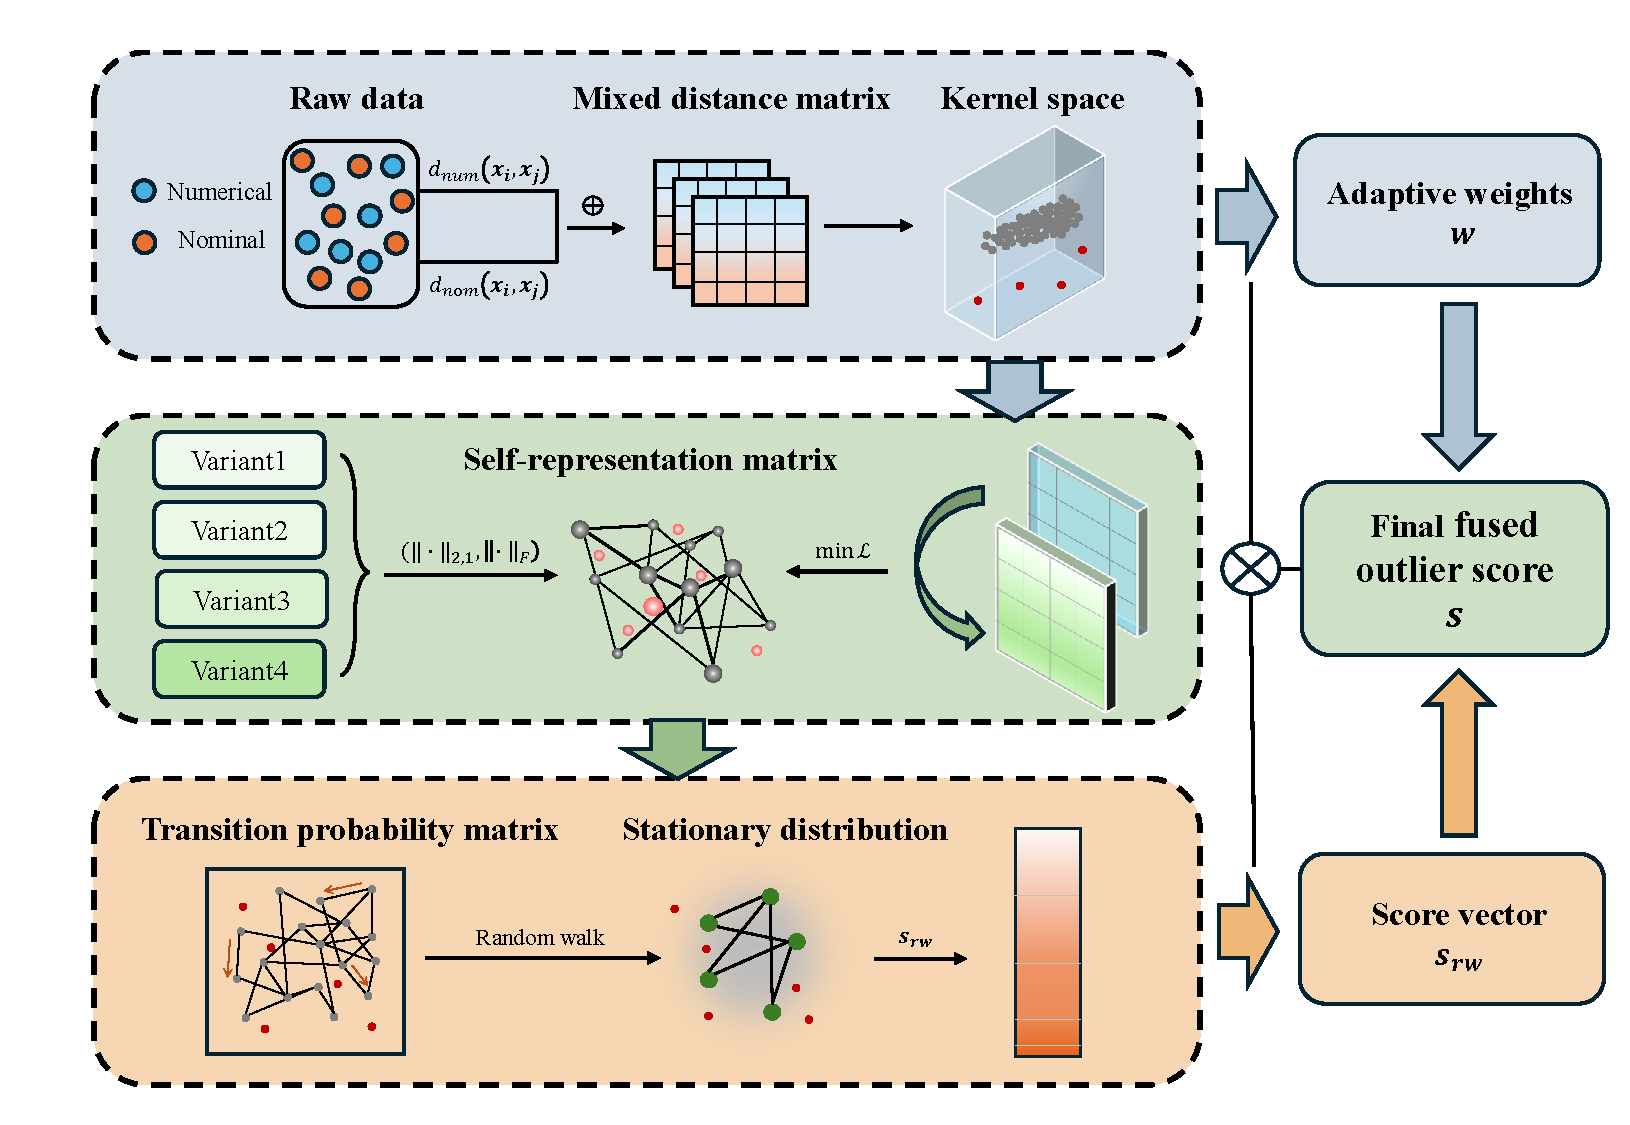
\includegraphics[width=\textwidth]{Figures/framework_KSRA.pdf} 
    \caption{The framework of KSRA.}
    \label{fig:KSRA_framework}
\end{figure*}


\begin{algorithm}
\caption{\enskip KSRA algorithm}\label{alg1}
\begin{algorithmic}
    \State \textbf{Input:} Data matrix $\boldsymbol{X} \in \mathbb{R}^{n \times m}$, regularization parameter $\lambda$.
    \State \textbf{Output:} Final outlier score $\boldsymbol{s}$.

    \State Compute the hybrid distance matrix $\boldsymbol{D}$
    \State Set the Gaussian bandwidth $\sigma = \frac{1}{n(n-1)}\sum_{i\ne j}d_{ij}$ and the restart probability $d=0.85$
    
    \State Construct the kernel matrix $\boldsymbol{K}$ by Eq.~(\ref{kernel_matrix})
    \State Compute the adaptive weights $w_{i}$ by Eq.~(\ref{initial_anomaly_belief})
    
    \State Initialize $\boldsymbol{Z}^{(0)}$, $t=0$
    
    \While{not converged \textbf{and} $t < T_{max}$}
        \State Update $\boldsymbol{Z}^{(t+1)}$ by Eqs.~(\ref{Case1}), (\ref{Case2}), (\ref{Case3}) or (\ref{Case4})
        \State $t = t + 1$
    \EndWhile
    
    \State Construct the transition matrix $\boldsymbol{P}$ by Eq.~(\ref{transition_probability})
    \State Compute the random walk steady-state score $\boldsymbol{s}_{rw}$ by Eq.~(\ref{randomwalk_outlier_score})
    \State Calculate the final fused outlier score $\boldsymbol{s}$ by Eq.~(\ref{fuse_outlier_score})
    
    \State \Return $\boldsymbol{s}$
\end{algorithmic}
\end{algorithm}

\section{Experiments}\label{Experiments}

In this section, we introduced the datasets and comparison algorithms employed, along with several experiments applied in our method. Analysis is conducted based on Receiver Operating
Characteristic (ROC) curves and Area Under the ROC
Curve (AUC) results, statistical hypothesis testing, and other aspects, with experimental findings visualized.

\subsection{Experiments Setup}

We select 20 public datasets spanning diverse domains and scales, encompassing numerical attribute data, nominal attribute data, and mixed attribute data. These datasets are accessible via the public website\footnote{\url{https://github.com/BELLoney/Outlier-detection}}. Basic information about the datasets is presented in Table \ref{KSRA-DS}. We used the prepared benchmark data files. Range-normalized columns in $[0,1]$ were processed using Euclidean distance, and the remaining integer-coded columns using normalized Hamming distance, with codes compared only for equality. In the prepared inputs, missing entries correspond to column-modal values for partially observed columns, while entirely missing columns are represented by constants. No additional imputation was performed during the experiments.

Also, we evaluate the performance of our method on 20 datasets in comparison with 11 representative anomaly detection algorithms, including AutoEncoder \cite{hinton2006reducing}, Variational AutoEncoder (VAE) \cite{kingma2013auto}, Variance Structural Score (VarE) \cite{8526528}, Weighted Neighbourhood Information Network based Outlier Detection (WNINOD) \cite{wang2021outlier}, Empirical-Cumulative-Distribution-based Outlier Detection (ECOD) \cite{li2022ecod}, Rotation-based Outlier Detection (ROD) \cite{almardeny2020novel}, Incomplete Local and Global Neighborhood Information (ILGNI) network \cite{li2023incomplete}, Deep Isolation Forest (DIF) \cite{xu2023deep}, Fusing Multi-scale Fuzzy Information to Detect Outliers (MFIOD) \cite{chen2024fusing}, Granule Density-based Anomaly Detection (GDAD) \cite{chen2025integrating}, and the Granular-ball Mean-shift Outlier Detector (GBMOD) \cite{cheng2025gbmod}. 

For these comparison methods, we set reasonable parameter ranges based on relevant papers to ensure favorable detection performance. For example, the hyper-parameter adjustment ranges of VarE varies in $\{10^i \mid i \in \{-3, -2, \dots, 3\}\}$, WNINOD in $[1,10]$, while GBMOD using $k \in[2,60]$ with a stepsize of 1. In the experimental settings for KSRA, the parameter $\lambda$ is selected from $\{10^j \mid j \in \{-8, -7, \dots, 6, 7\}\}$ with a logarithmic increment of 10. Model fitting does not use anomaly labels. For the reported benchmark results, $\lambda$ is selected by the highest evaluation ROC-AUC within the specified grid. The bandwidth $\sigma$ is determined from the unlabeled input, while the restart weight is fixed at $d=0.85$. Sensitivity analyses characterize parameter effects but do not replace a label-independent selection procedure.

We employ the ROC curve and the AUC as the primary evaluation metrics \cite{campos2016evaluation}. The ROC curve illustrates the trade-off between the True Positive Rate (TPR) and the False Positive Rate (FPR) across various decision thresholds. The AUC value, representing the area under the ROC curve, provides a scalar measure of the overall classification performance. An AUC value closer to 1 indicates a superior capability of the algorithm to correctly rank anomalous instances higher than normal ones. Stochastic baselines were evaluated using single runs; their reported results do not quantify variability across random seeds.


\begin{table*}[!ht]
	\caption{Basic information of experimental datasets.}\label{KSRA-DS}
    \centering
	% \resizebox{1\textwidth}{!}{
		\begin{tabular}{lllccccc}
			\toprule
			ID & Datasets & Abbr. & Type & Attributes & Objects & Outliers & Outlier ratios \\\midrule
            1 & Annealing\_variant1 & Annealing & Mixed & 38 & 798 & 42 & 5.26\% \\
            2 & Arrhythmia\_variant1 & Arrhythmia & Mixed & 279 & 452 & 66 & 14.60\% \\
            3 & Audiology\_variant1 & Audio & Nominal & 69 & 226 & 57 & 25.22\% \\
            4 & Bands\_band\_6\_variant1 & Bands & Mixed & 39 & 318 & 6 & 1.89\% \\
            5 & Cardio & Cardio & Mixed & 21 & 1831 & 176 & 9.61\% \\
            6 & Cardiotocography\_2and3\_33\_variant1 & Cardio\_33 & Mixed & 21 & 1688 & 33 & 1.95\% \\
            7 & Chess\_nowin\_16\_variant1 & Chess\_16 & Nominal & 36 & 1685 & 16 & 0.95\% \\
            8 & Chess\_nowin\_34\_variant1 & Chess\_34 & Nominal & 36 & 1703 & 34 & 2.00\% \\
            9 & Ecoli & Ecoli & Mixed & 7 & 336 & 9 & 2.68\% \\
            10 & Iris\_Irisvirginica\_11\_variant1 & Iris & Numerical & 4 & 111 & 11 & 9.91\% \\
            11 & Lymphography & Lymphography & Nominal & 18 & 148 & 6 & 4.05\% \\
            12 & Monks\_0\_4\_variant1 & Monks & Nominal & 6 & 232 & 4 & 1.72\% \\
            13 & Mushroom\_p\_221\_variant1 & Mushroom & Mixed & 22 & 4429 & 221 & 4.99\% \\
            14 & Sick\_sick\_72\_variant1 & Sick & Mixed & 29 & 3613 & 72 & 1.99\% \\
            15 & Tic\_tac\_toe\_negative\_12\_variant1 & Tic\_12 & Nominal & 9 & 638 & 12 & 1.88\% \\
            16 & Tic\_tac\_toe\_negative\_32\_variant1 & Tic\_32 & Nominal & 9 & 658 & 32 & 4.86\% \\
            17 & Vote\_republican\_29\_variant1 & Vote & Nominal & 16 & 296 & 29 & 9.80\% \\
            18 & Wbc\_malignant\_39\_variant1 & Wbc & Nominal & 9 & 483 & 39 & 8.07\% \\
            19 & Wdbc\_M\_39\_variant1 & Wdbc\_M & Numerical & 31 & 396 & 39 & 9.85\% \\
            20 & Yeast\_ERL\_5\_variant1 & Yeast & Mixed & 8 & 1141 & 5 & 0.44\% \\
            \bottomrule
        \end{tabular}
        % }
\end{table*}


\subsection{Experimental Results}

The ROC curves in the experimental results are shown in Fig.\ref{fig:all_rocs}. Our KSRA method is highlighted in red among all. A ROC curve situated closer to the upper-left corner indicates a more ideal performance. Consequently, it can be intuitively observed from the figure that our proposed method achieves significant superiority over the competing methods on the Annealing, Audio, Ecoli and Tic\_32 datasets, demonstrating a remarkable margin of improvement. Meanwhile, it generally outperforms other baseline methods on Arrhythmia, Cardio\_33 and Monks.

Table \ref{KSRA-AUC} provides more detailed and easily comparable AUC metric results, where the optimal result on each dataset is displayed in bold, and the second-best result is indicated by underlining. Here, KSRA$_1$ through KSRA$_4$ represent the variants obtained via different combinations of paradigms discussed in the Sample Self-representation section (see Section \ref{Variant Analysis} for details). KSRA$_2$ serves as the fixed variant for the main comparison across datasets. KSRA$_{best}$ is an oracle reference and is excluded from fixed-method rankings and statistical tests. Based on the results in the table, we can draw the following conclusions:

\begin{enumerate}[\indent (1)]
    \item KSRA demonstrates outstanding overall performance across 20 benchmark datasets, achieving the best AUC values on a total of 14 datasets. Its overall average AUC $0.954$ is significantly better than that of 11 mainstream comparison algorithms. Although our algorithm achieved second-best results on the Cardio, Chess\_34, and Mushroom datasets, the gap in metrics compared to the best-performing algorithms was less than 0.01, indicating essentially equivalent performance.
    \item In an internal comparison of the four KSRA variants, KSRA$_2$ achieved the best average AUC of 0.951, with KSRA$_3$ performing closely behind and demonstrating stable detection accuracy. KSRA$_1$ and KSRA$_4$ also exhibit good generalization capabilities, which is able to adapt to different data scenarios.
    \item Although KSRA did not achieve the best result on Sick and Wdbc\_M, its performance remained highly competitive. In particular, the performance gap on Wdbc\_M was negligible. For Sick, the extremely low outlier ratio makes anomaly samples highly isolated within the sample graph. Under such circumstances, the random walk process tends to be dominated by the overwhelming majority of normal samples, which may weaken the propagation of anomaly-related information. In addition, Sick is a relatively low-dimensional dataset. Therefore, the advantage brought by kernel-based nonlinear representation may be less pronounced than on datasets exhibiting stronger nonlinear or high-dimensional characteristics.
\end{enumerate}
Overall, the proposed framework offers clear advantages over existing methods in scenarios involving mixed attributes and high-dimensional data.

To complement the original comparison, we evaluate the four KSRA variants against a recent deep graph anomaly detector, DVGAE-GAN \cite{khan2024anomalous}, together with established kernel-based methods, Kernel PCA \cite{hoffmann2007kernel} and OCSVM-RBF \cite{scholkopf2001estimating}, and the low-rank self-representation method LRR \cite{liu2012exact}. All methods are evaluated on the 20 benchmark datasets. The four variants employ different combinations of reconstruction losses and regularization terms, and their results are reported separately in Table \ref{tab:additional_baselines} to examine the performance
of the different formulations. Additionally, KSRA$_{best}$ denotes the highest AUC among the four variants on each dataset. It serves only as an oracle best-variant reference, rather than an independently specified method.

KSRA$_2$ and KSRA$_3$ achieve mean AUC of 0.9509 and
0.9504, respectively, exceeding those of the other two variants and all four additional baselines. The mean AUC of KSRA$_{best}$ reaches 0.9537. These results reveal differences among the objective formulations, with KSRA$_2$ and KSRA$_3$ providing favorable overall performance. The findings can be summarized as follows:

\begin{enumerate}[\indent (1)]
    \item KSRA$_2$ achieves the highest mean AUC among the
    four fixed variants, closely followed by KSRA$_3$.
    Their mean AUCs exceed that of the strongest additional baseline, OCSVM-RBF, by 1.23 and 1.18 percentage points, respectively.

    \item KSRA$_1$ and KSRA$_4$ obtain mean AUC of
    0.9319 and 0.9350. Both exceed DVGAE-GAN,
    Kernel PCA, and LRR, but remain below OCSVM-RBF.
    Thus, not every KSRA formulation provides the same
    level of overall performance.

    \item KSRA$_{best}$ achieves the best or joint-best AUC
    on 16 datasets, with a mean AUC of 0.9537.
    Its mean exceeds that of fixed KSRA$_2$ by 0.0028.
    This difference quantifies the observed benefit of
    per-dataset variant selection, but should not be
    interpreted as the performance of a fixed method.

    \item Kernel PCA or OCSVM-RBF outperforms all four
    KSRA variants on Bands, Chess\_16, Chess\_34,
    and Mushroom. These exceptions demonstrate that
    conventional kernel methods remain competitive
    on particular datasets.
\end{enumerate}



\begin{figure*}[t!]
  \centering
  % =================== 第一行 (1-4) ===================
  \begin{minipage}[b]{0.24\textwidth}
    \centering
    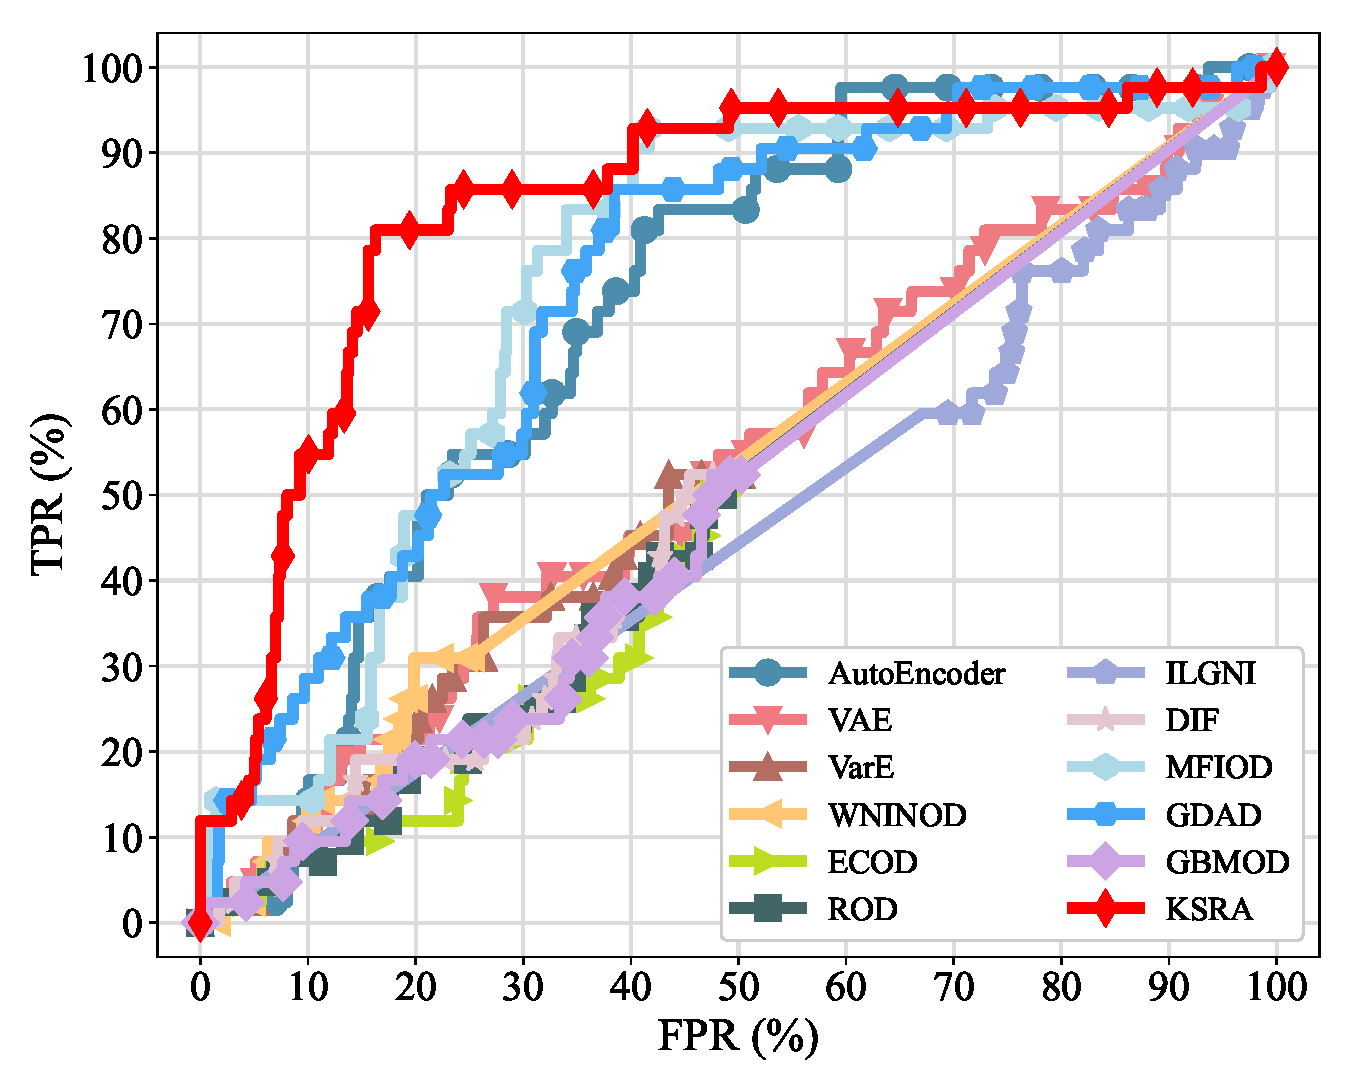
\includegraphics[width=\textwidth]{Figures/annealing_variant1_ROC.eps}
    \small (a) Annealing 
    \label{fig:Annealing}
  \end{minipage}
  \hfill
  \begin{minipage}[b]{0.24\textwidth}
    \centering
    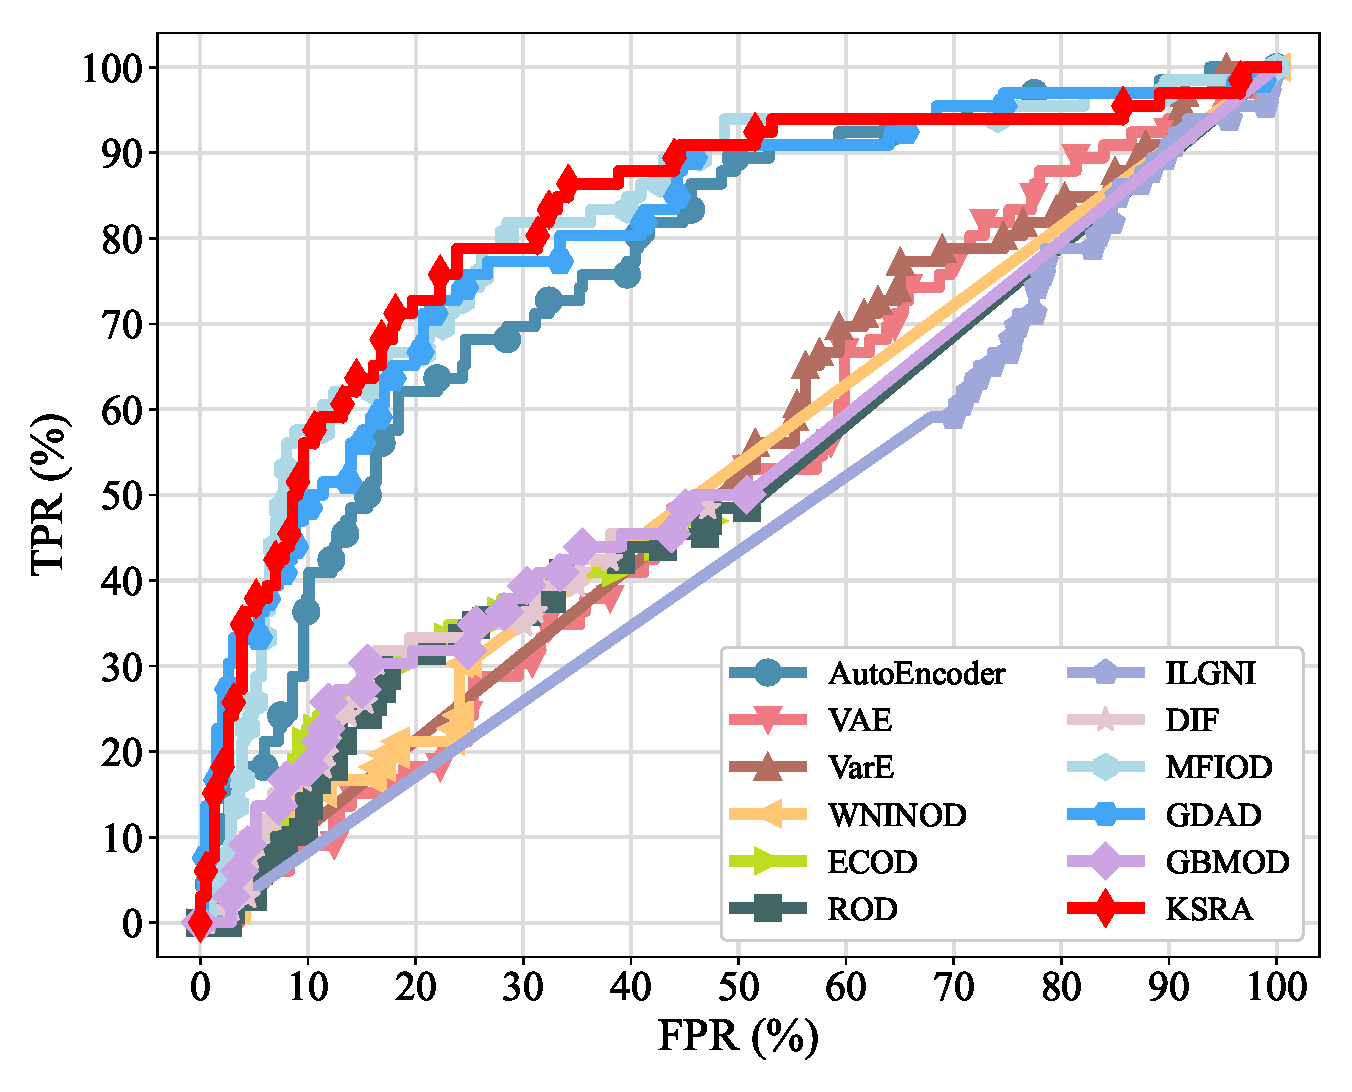
\includegraphics[width=\textwidth]{Figures/arrhythmia_variant1_ROC.eps}
    \small (b) Arrhythmia
    \label{fig:Arrhythmia}
  \end{minipage}
  \hfill
  \begin{minipage}[b]{0.24\textwidth}
    \centering
    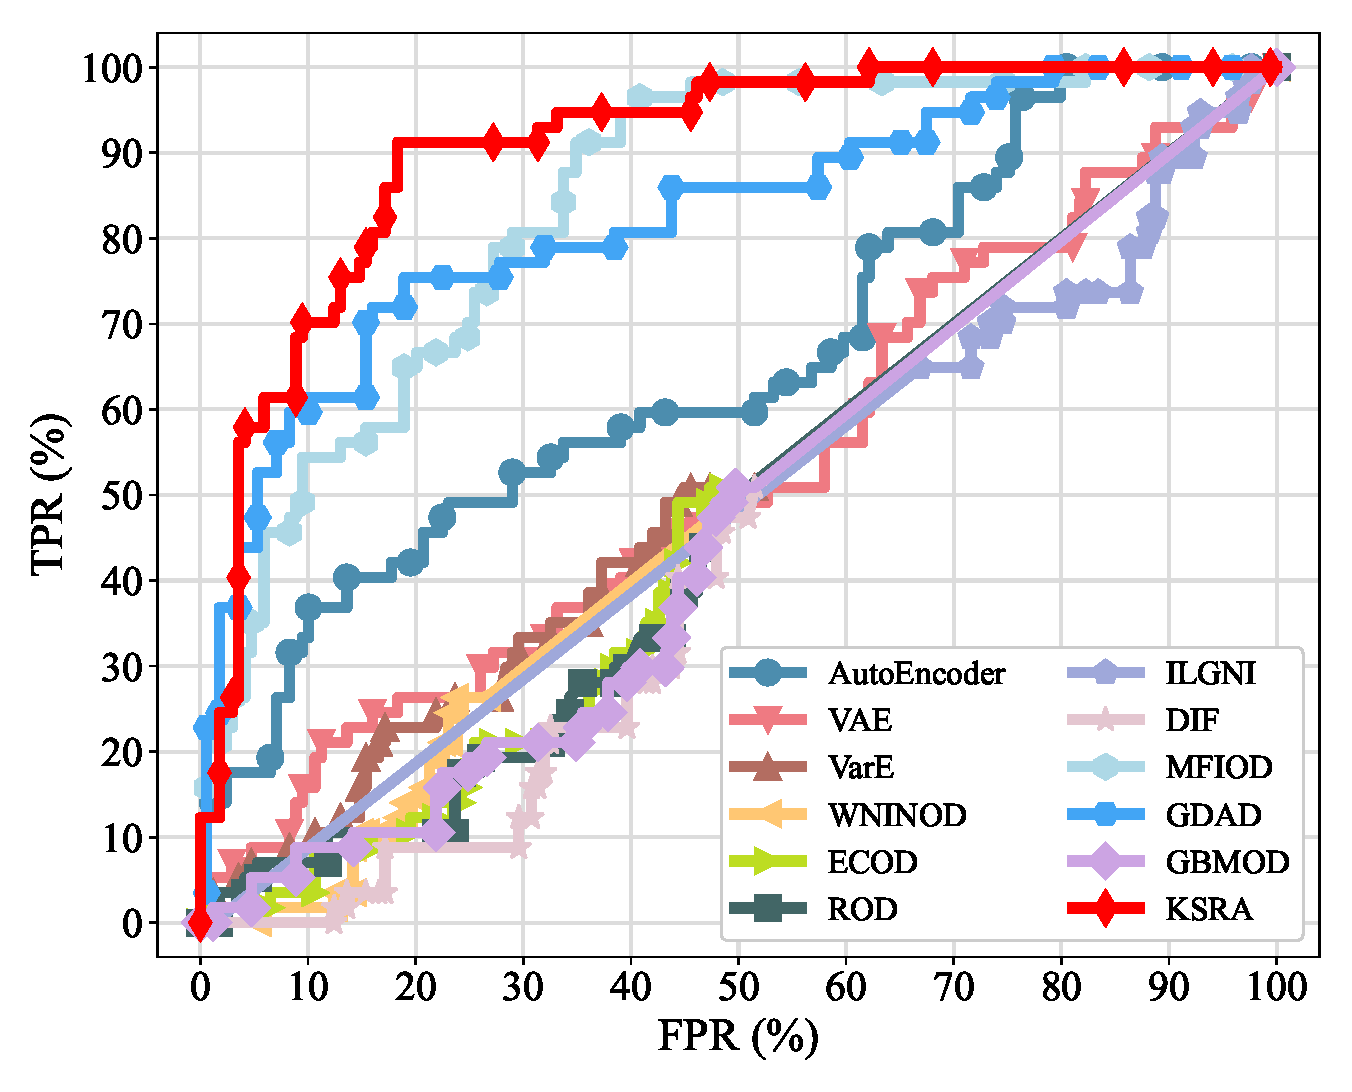
\includegraphics[width=\textwidth]{Figures/audiology_variant1_ROC.eps}
    \small (c) Audio
    \label{fig:Audio}
  \end{minipage}
  \hfill
  \begin{minipage}[b]{0.24\textwidth}
    \centering
    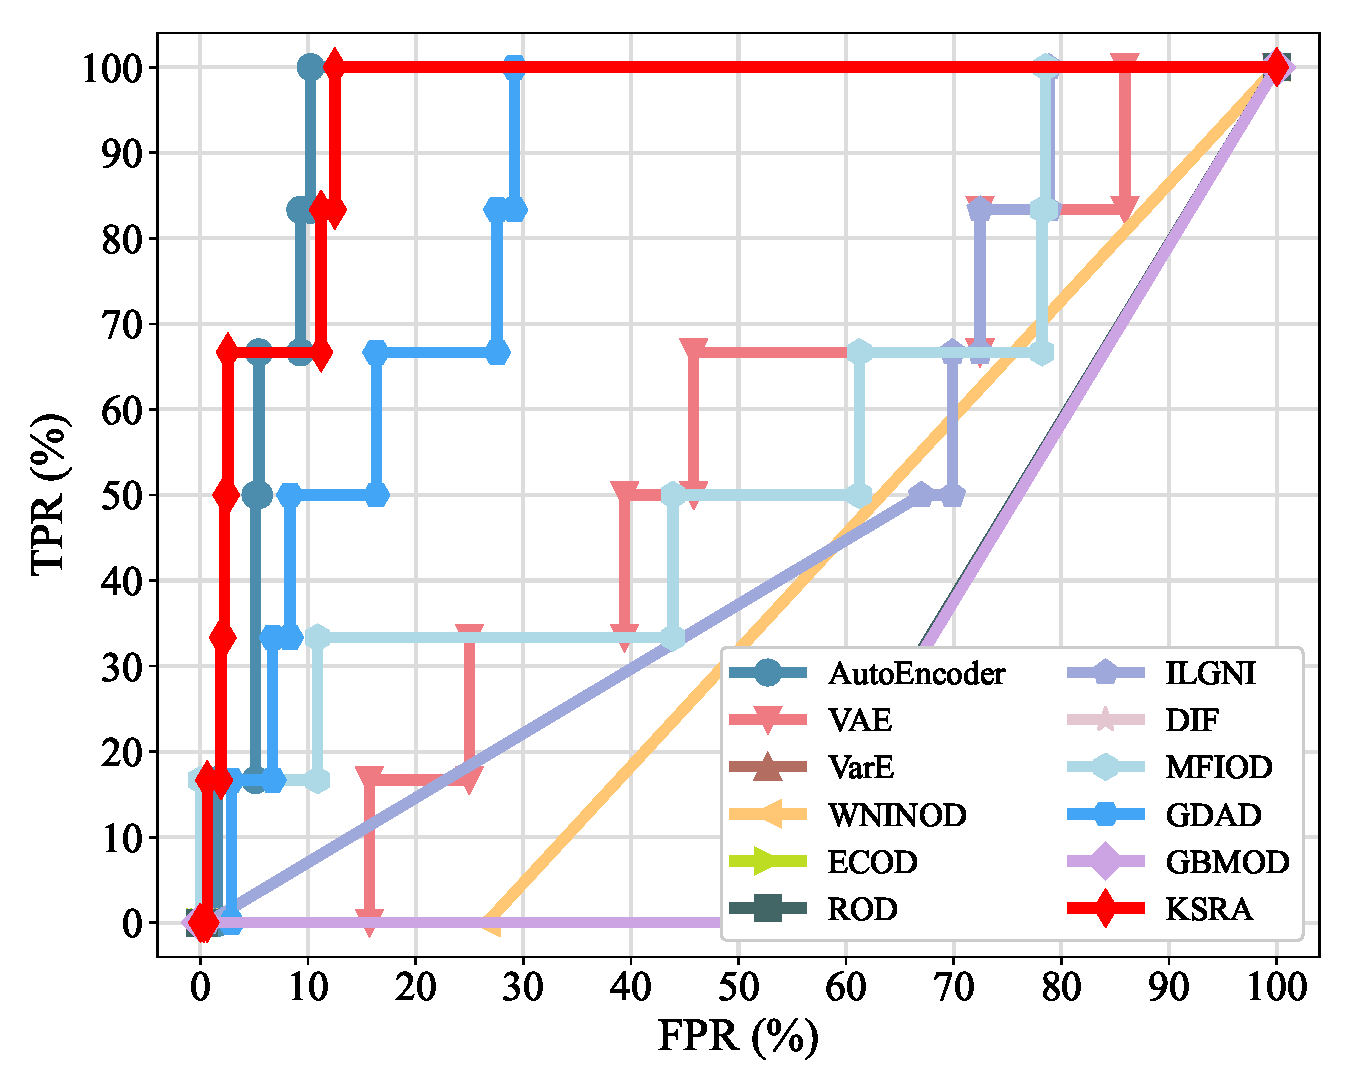
\includegraphics[width=\textwidth]{Figures/bands_band_6_variant1_ROC.eps}
    \small (d) Bands
    \label{fig:Bands}
  \end{minipage}

  \vspace{10pt} % 行与行之间的间距

  % =================== 第二行 (5-8) ===================
  \begin{minipage}[b]{0.24\textwidth}
    \centering
    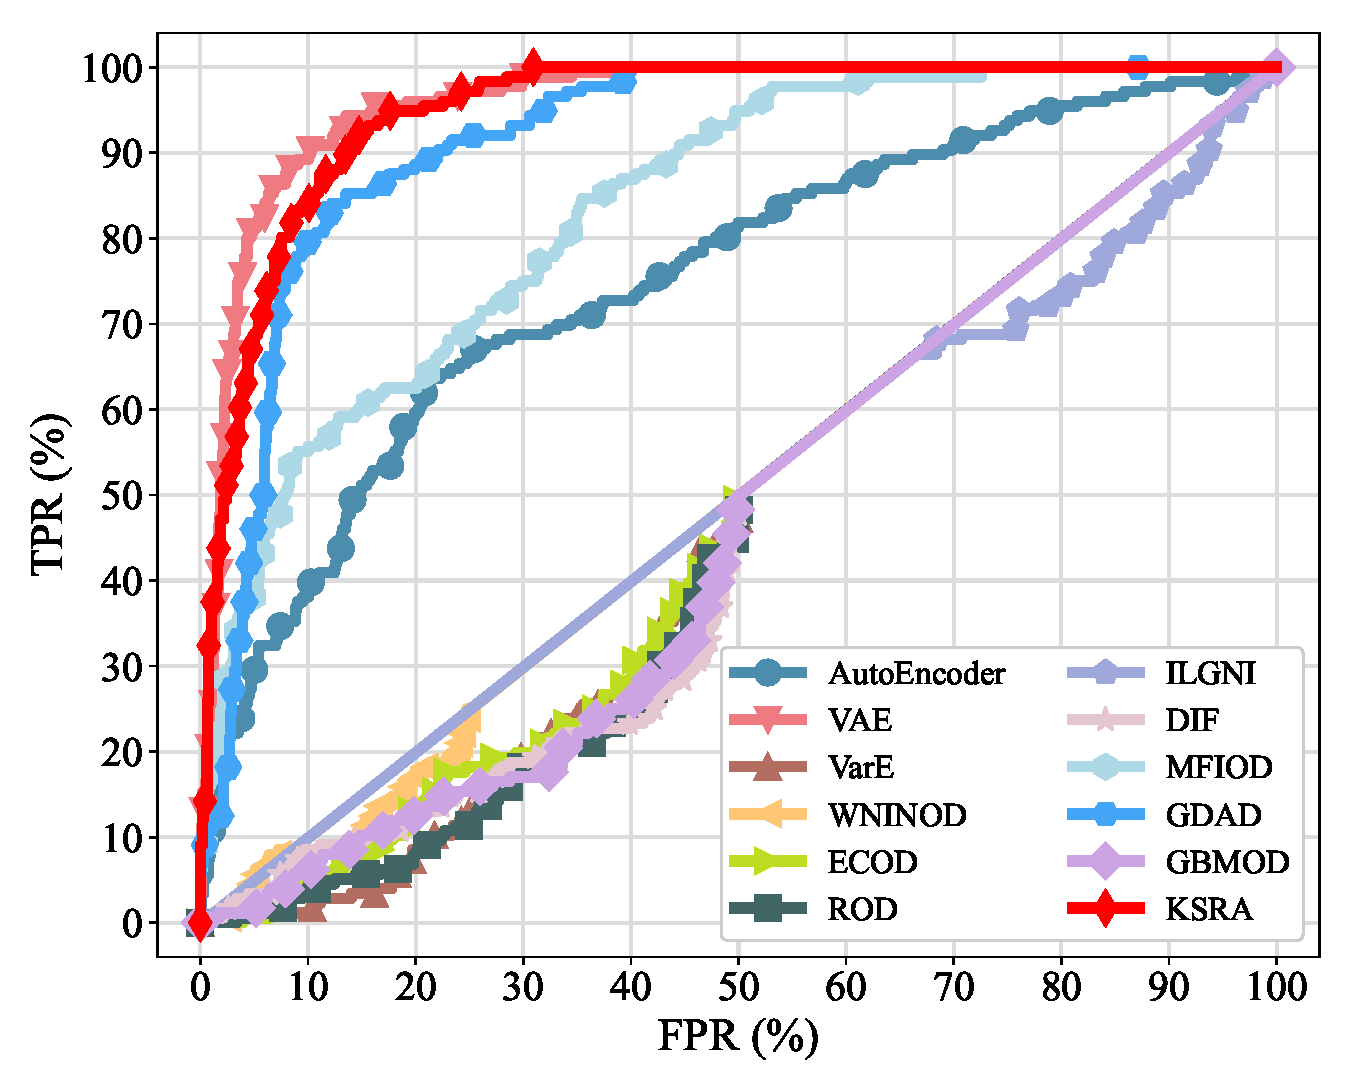
\includegraphics[width=\textwidth]{Figures/cardio_ROC.eps}
    \small (e) Cardio
    \label{fig:Cardio}
  \end{minipage}
  \hfill
  \begin{minipage}[b]{0.24\textwidth}
    \centering
    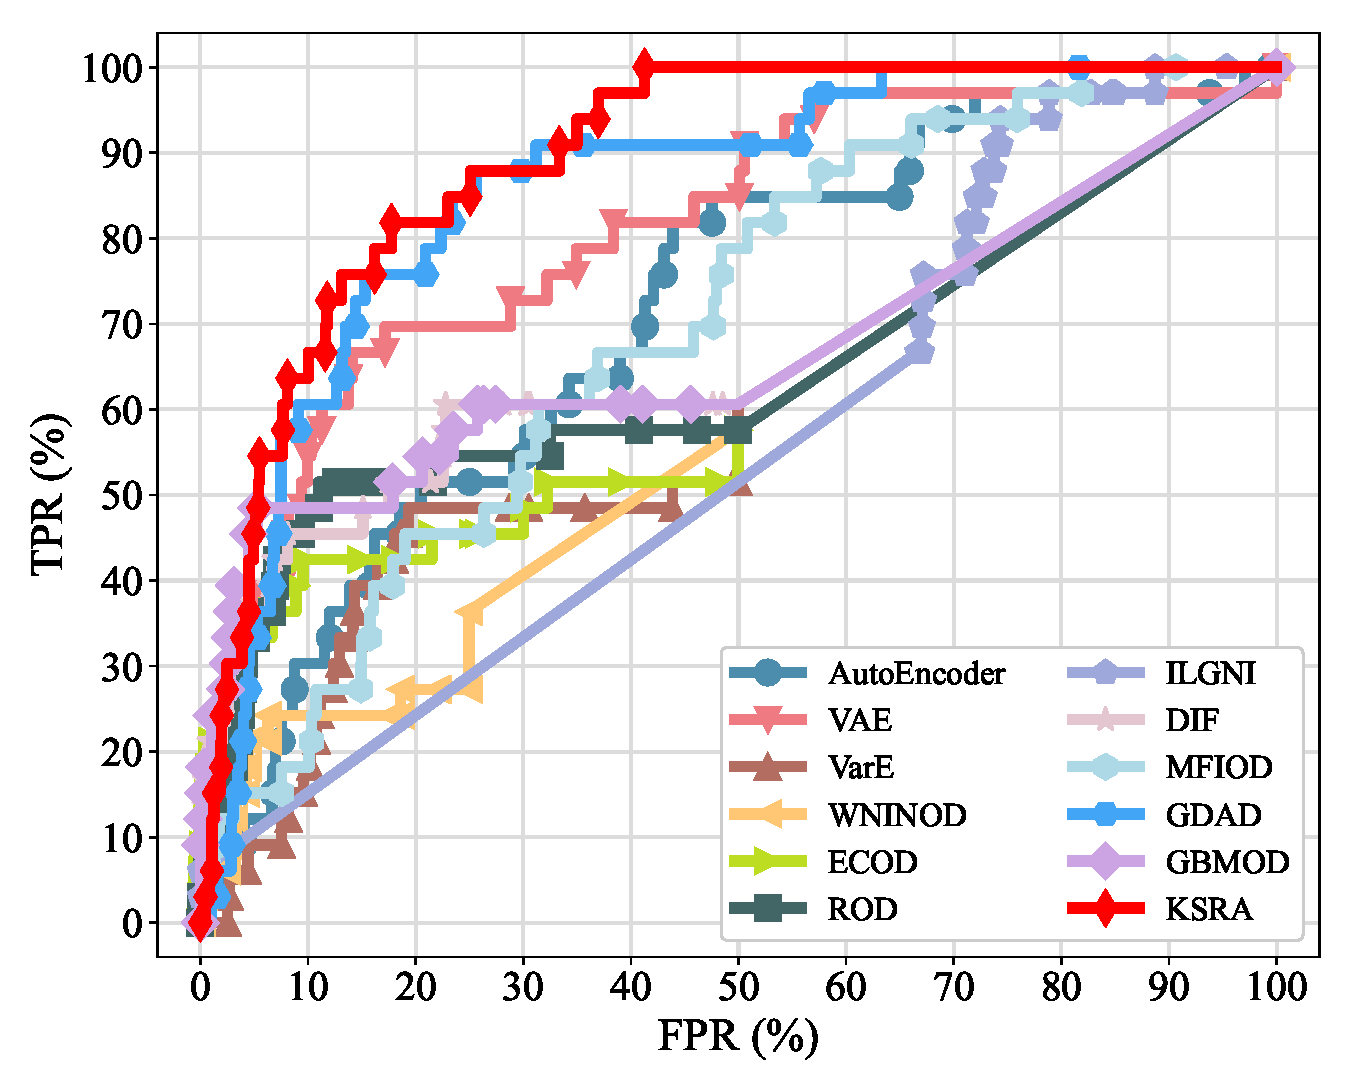
\includegraphics[width=\textwidth]{Figures/cardiotocography_2and3_33_variant1_ROC.eps}
    \small (f) Cardio\_33
    \label{fig:Cardio_33}
  \end{minipage}
  \hfill
  \begin{minipage}[b]{0.24\textwidth}
    \centering
    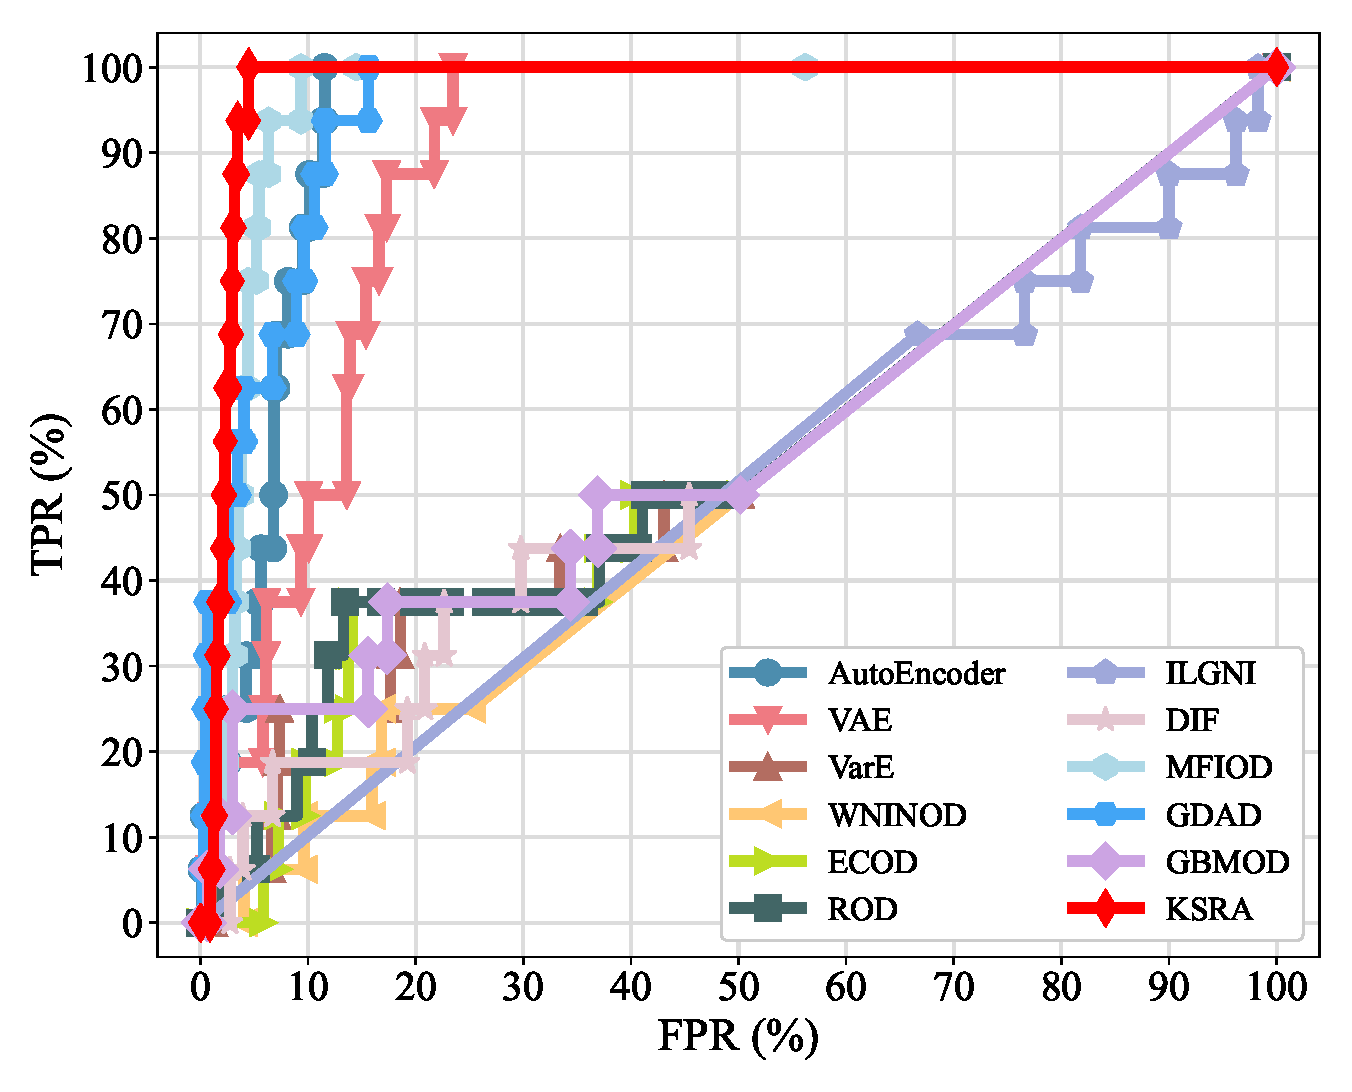
\includegraphics[width=\textwidth]{Figures/chess_nowin_16_variant1_ROC.eps}
    \small (g) Chess\_16
    \label{fig:Chess_16}
  \end{minipage}
  \hfill
  \begin{minipage}[b]{0.24\textwidth}
    \centering
    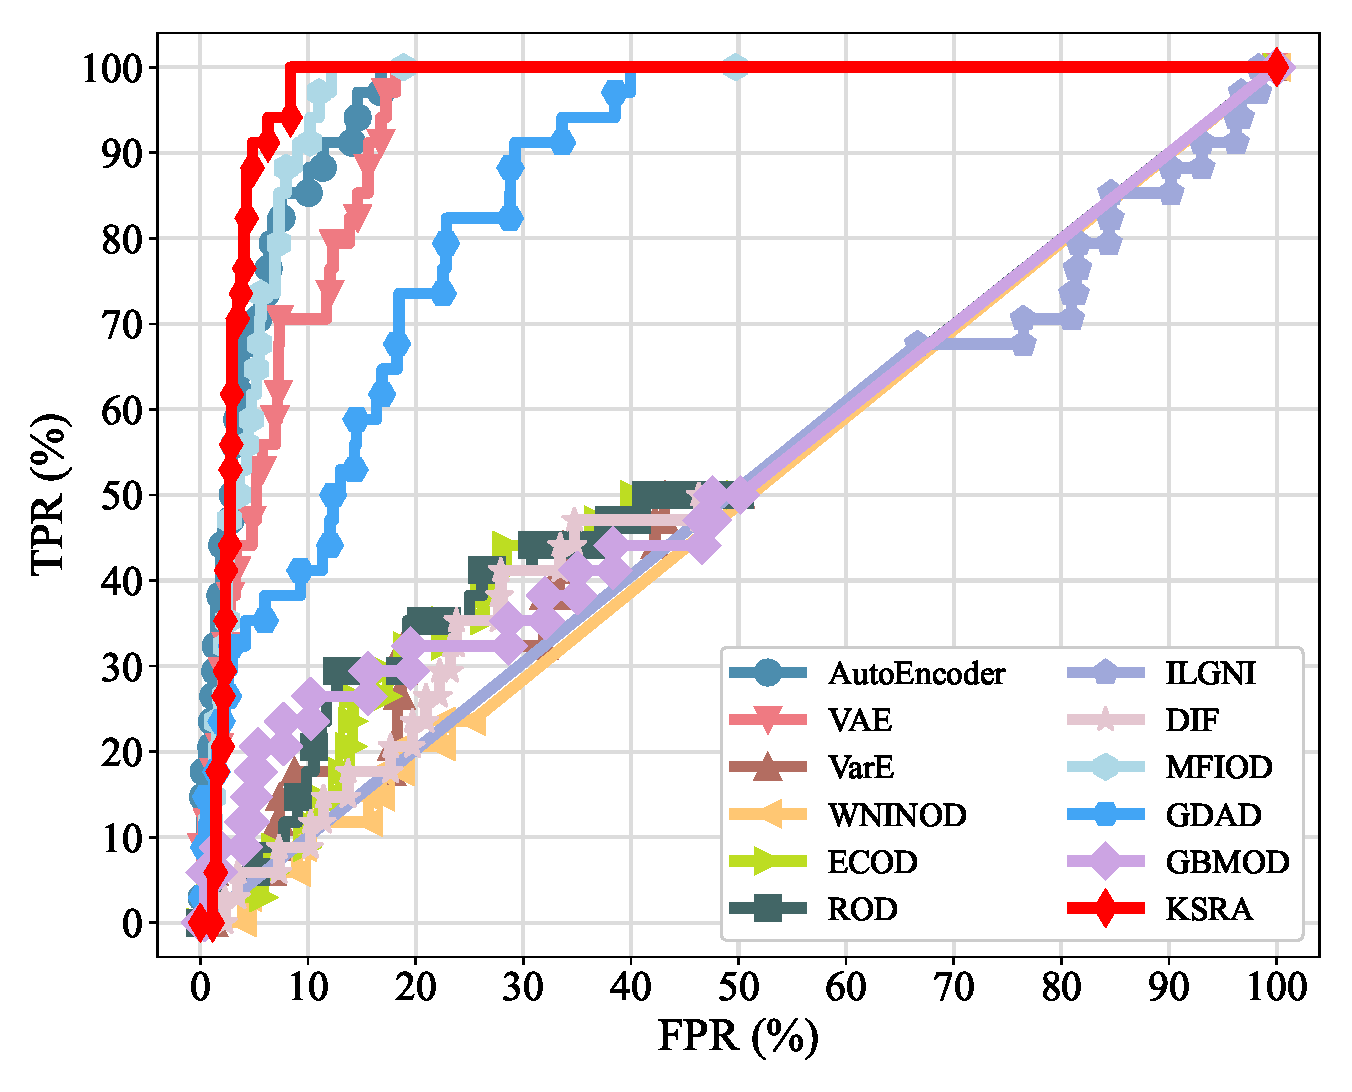
\includegraphics[width=\textwidth]{Figures/chess_nowin_34_variant1_ROC.eps}
    \small (h) Chess\_34
    \label{fig:Chess_34}
  \end{minipage}

  \vspace{10pt}

  % =================== 第三行 (9-12) ===================
  \begin{minipage}[b]{0.24\textwidth}
    \centering
    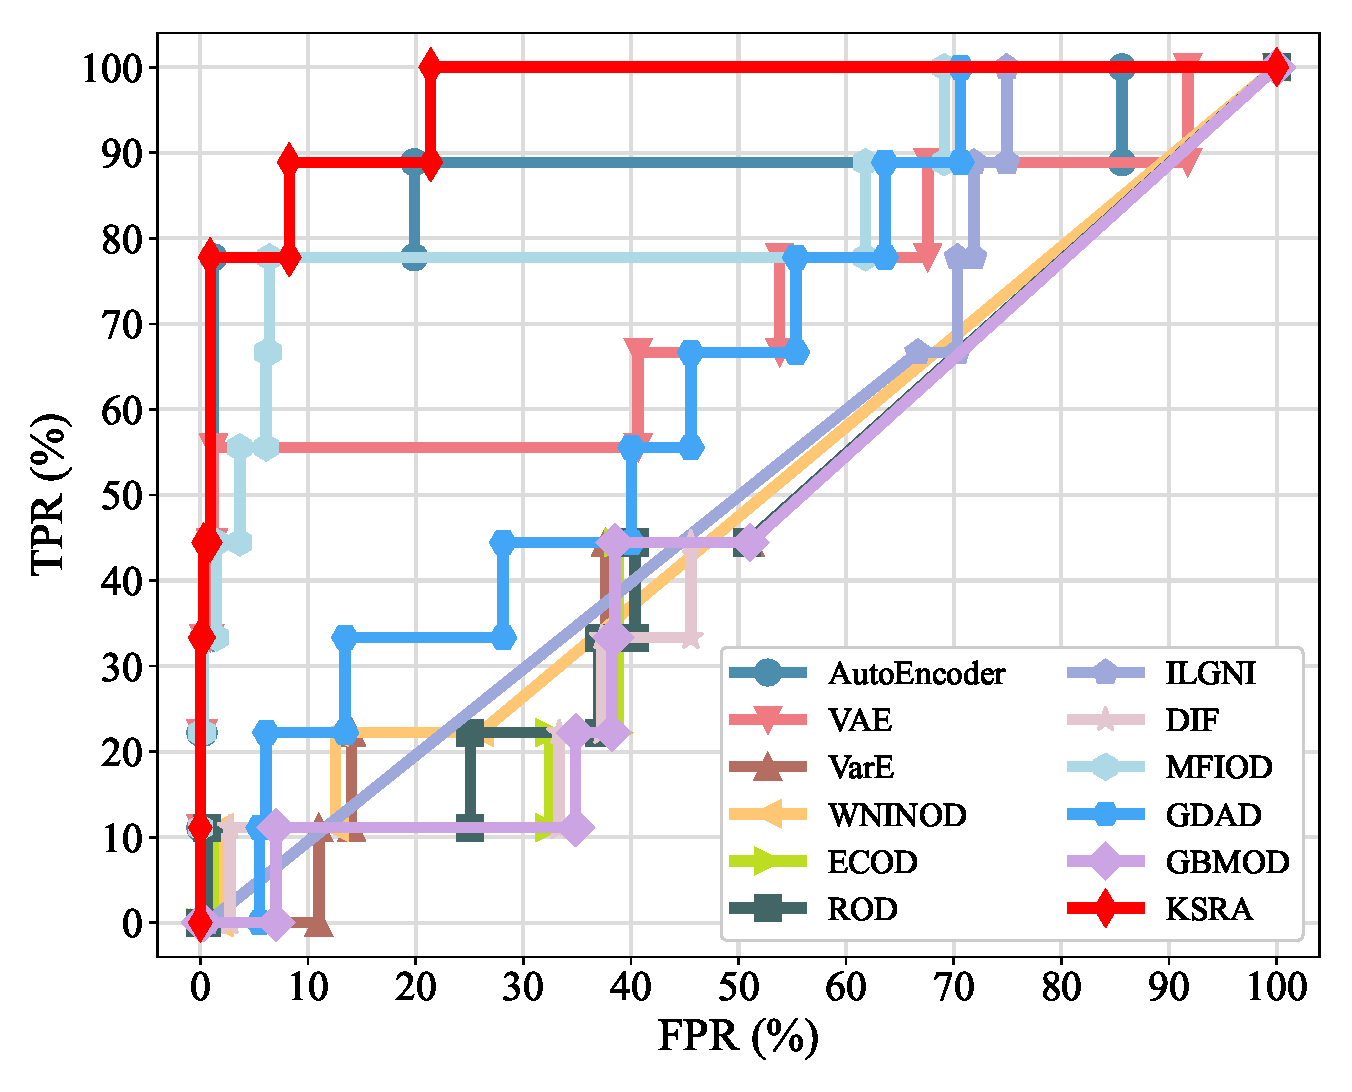
\includegraphics[width=\textwidth]{Figures/ecoli_ROC.eps}
    \small (i) Ecoli
    \label{fig:Ecoli}
  \end{minipage}
  \hfill
  \begin{minipage}[b]{0.24\textwidth}
    \centering
    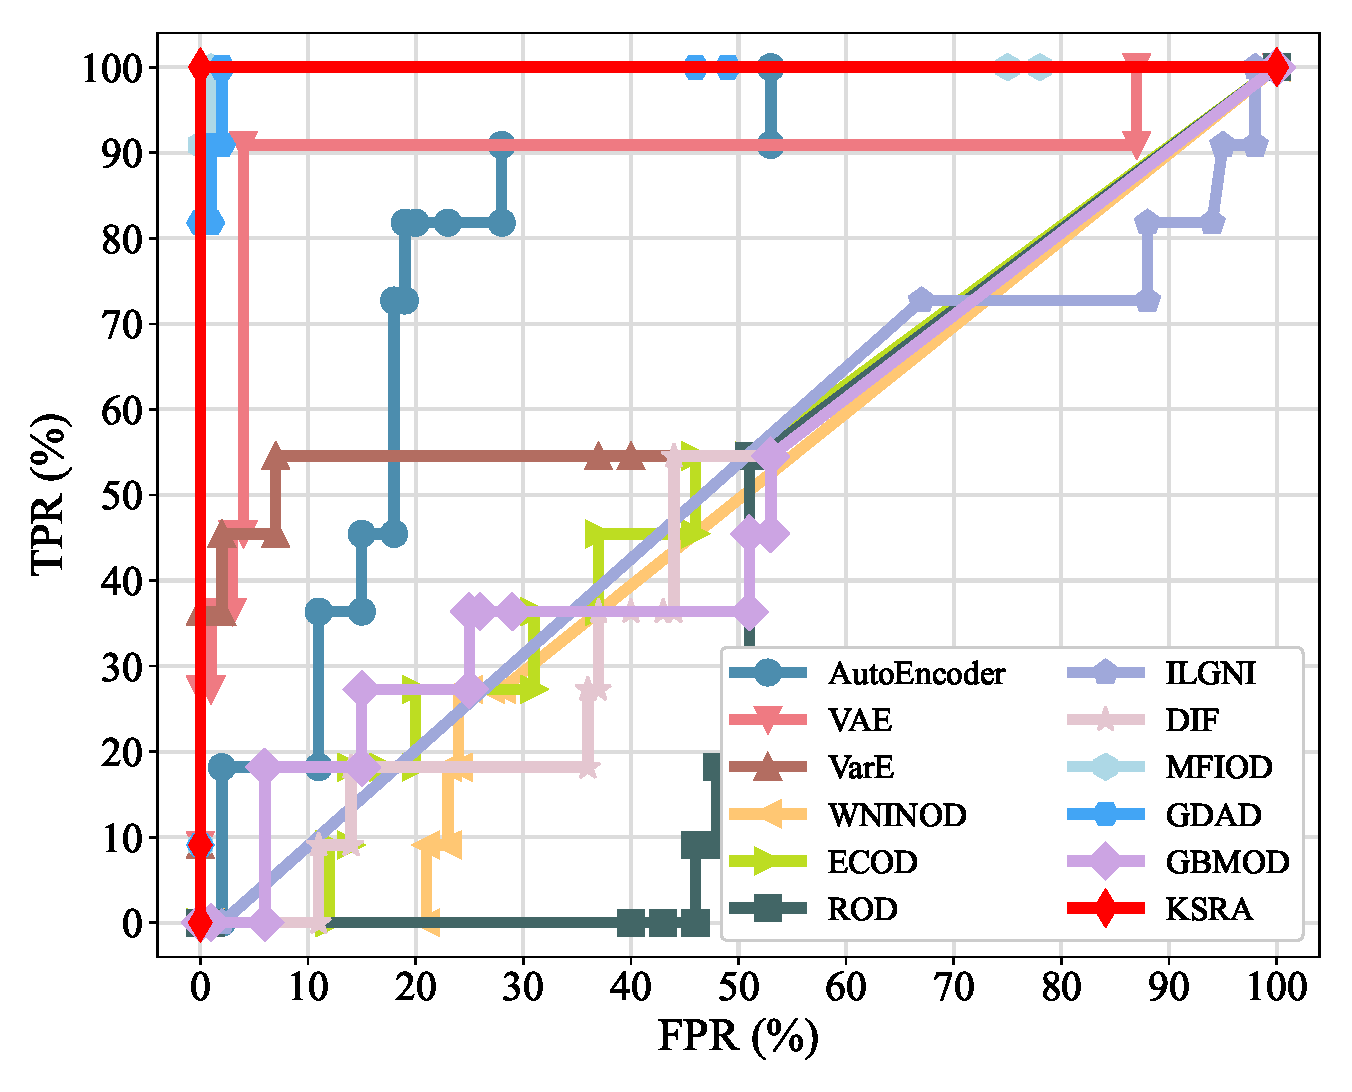
\includegraphics[width=\textwidth]{Figures/iris_Irisvirginica_11_variant1_ROC.eps}
    \small (j) Iris
    \label{fig:Iris}
  \end{minipage}
  \hfill
  \begin{minipage}[b]{0.24\textwidth}
    \centering
    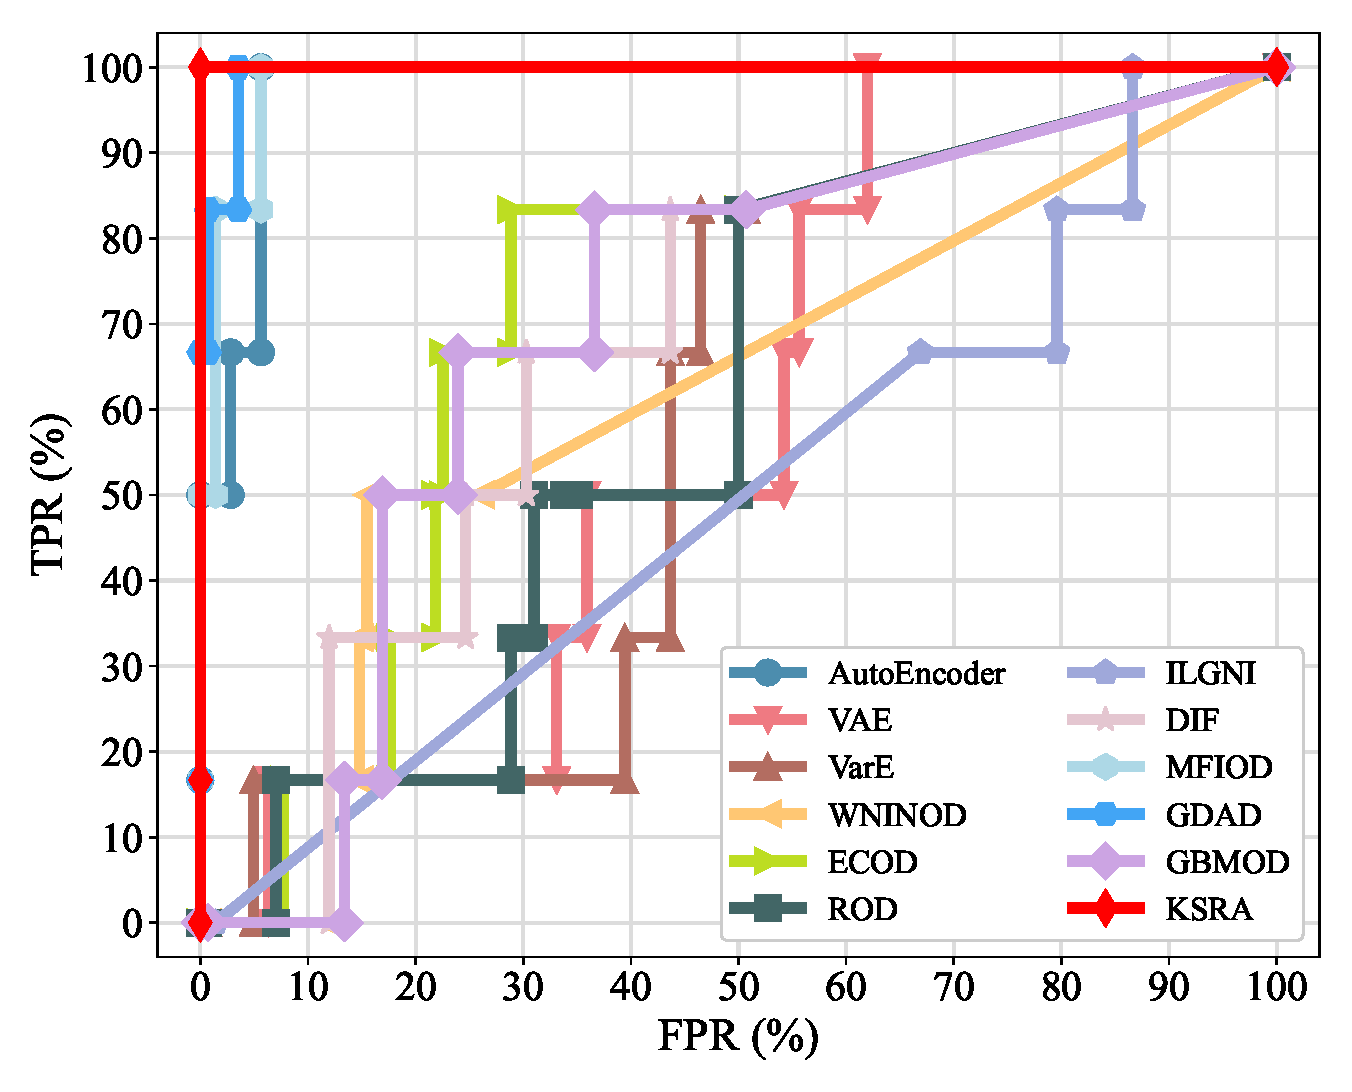
\includegraphics[width=\textwidth]{Figures/lymphography_ROC.eps}
    \small (k) Lymphography
    \label{fig:Lymphography}
  \end{minipage}
  \hfill
  \begin{minipage}[b]{0.24\textwidth}
    \centering
    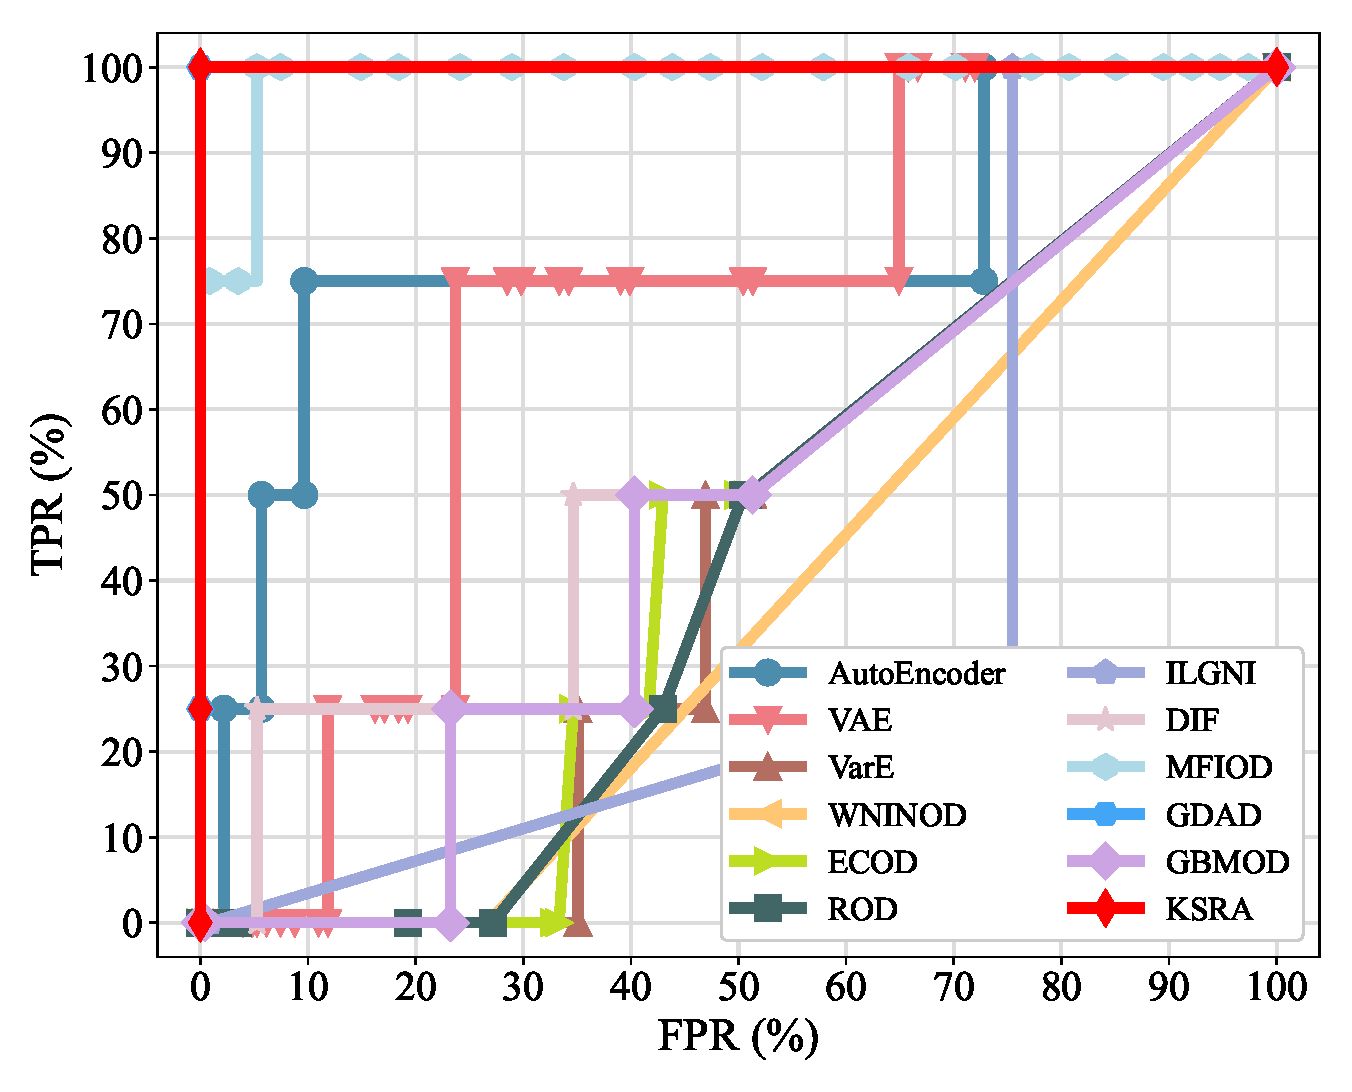
\includegraphics[width=\textwidth]{Figures/monks_0_4_variant1_ROC.eps}
    \small (l) Monks
    \label{fig:Monks}
  \end{minipage}

  \vspace{10pt}

  % =================== 第四行 (13-16) ===================
  \begin{minipage}[b]{0.24\textwidth}
    \centering
    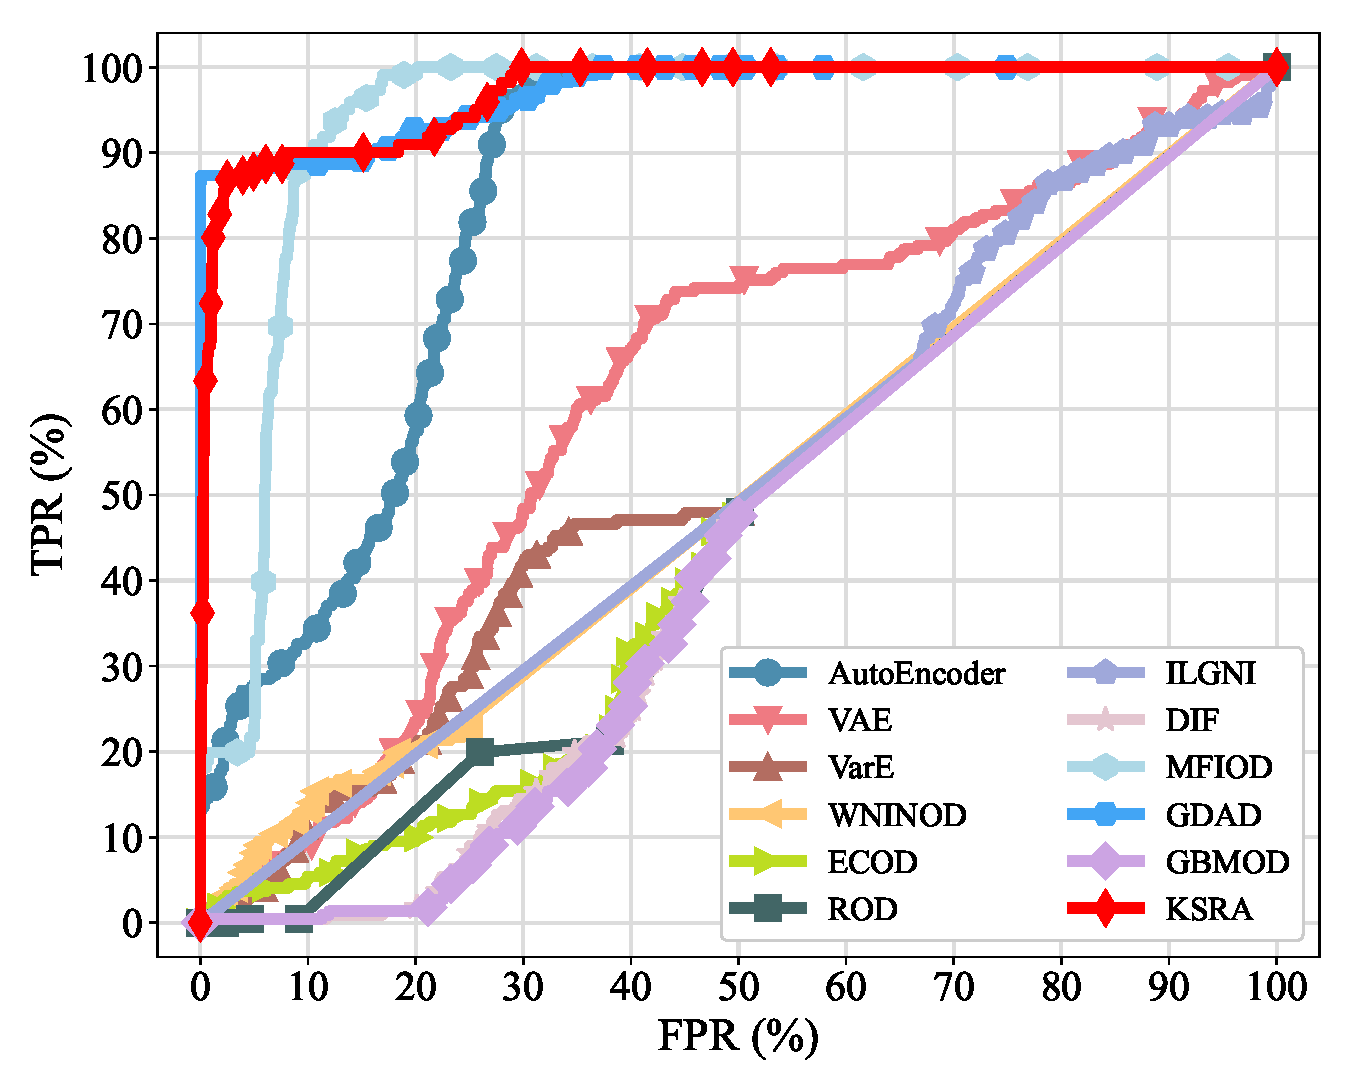
\includegraphics[width=\textwidth]{Figures/mushroom_p_221_variant1_ROC.eps}
    \small (m) Mushroom
    \label{fig:Mushroom}
  \end{minipage}
  \hfill
  \begin{minipage}[b]{0.24\textwidth}
    \centering
    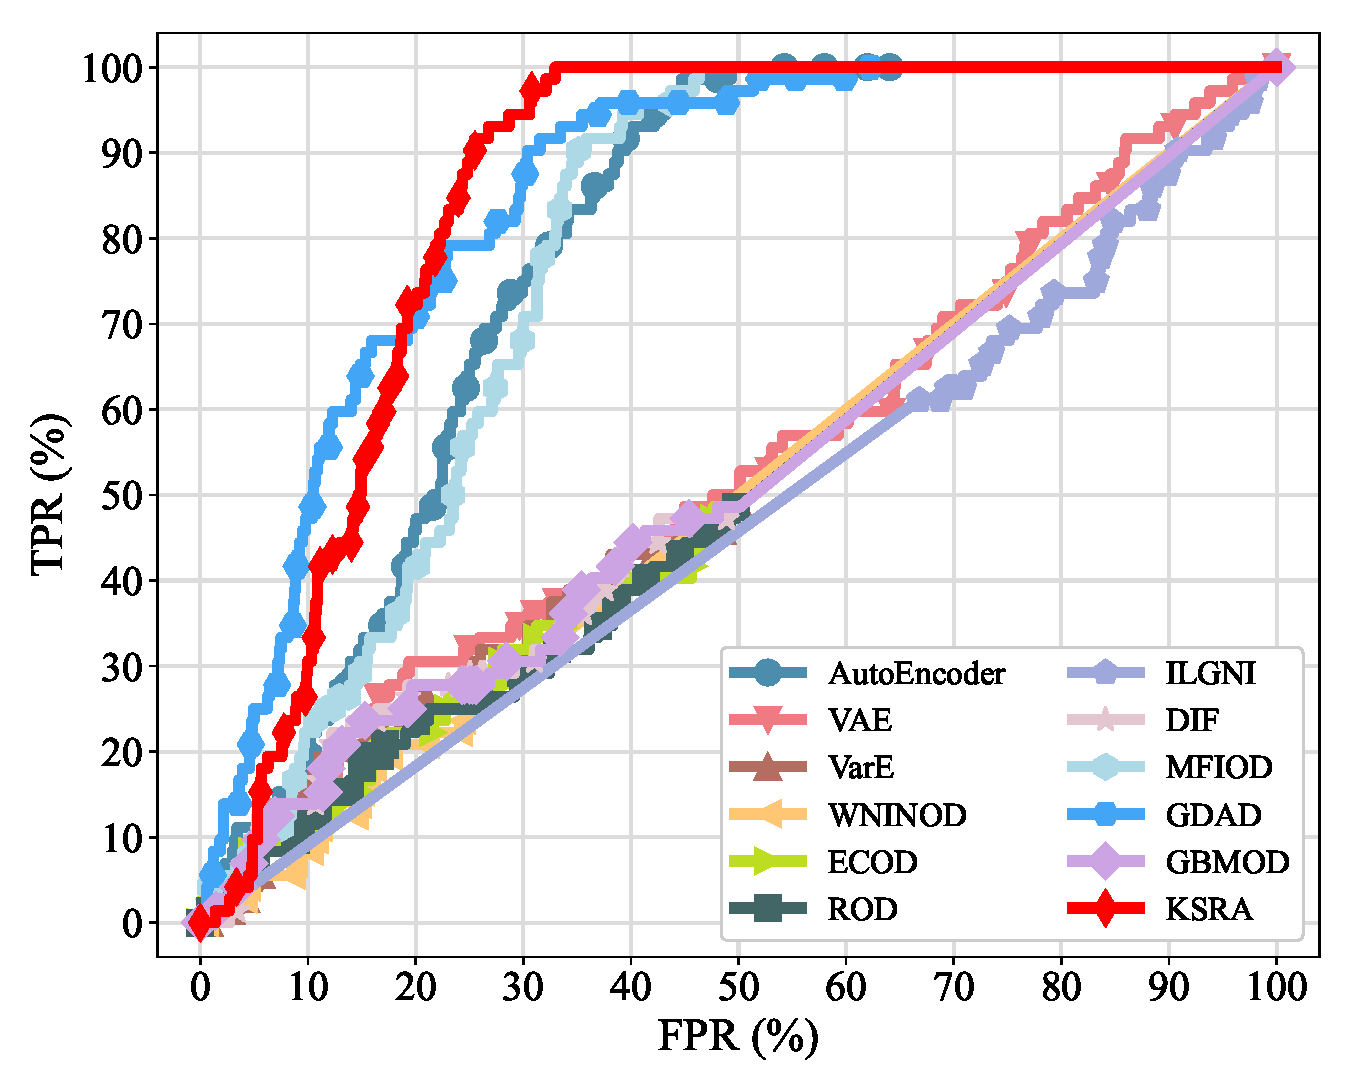
\includegraphics[width=\textwidth]{Figures/sick_sick_72_variant1_ROC.eps}
    \small (n) Sick
    \label{fig:Sick}
  \end{minipage}
  \hfill
  \begin{minipage}[b]{0.24\textwidth}
    \centering
    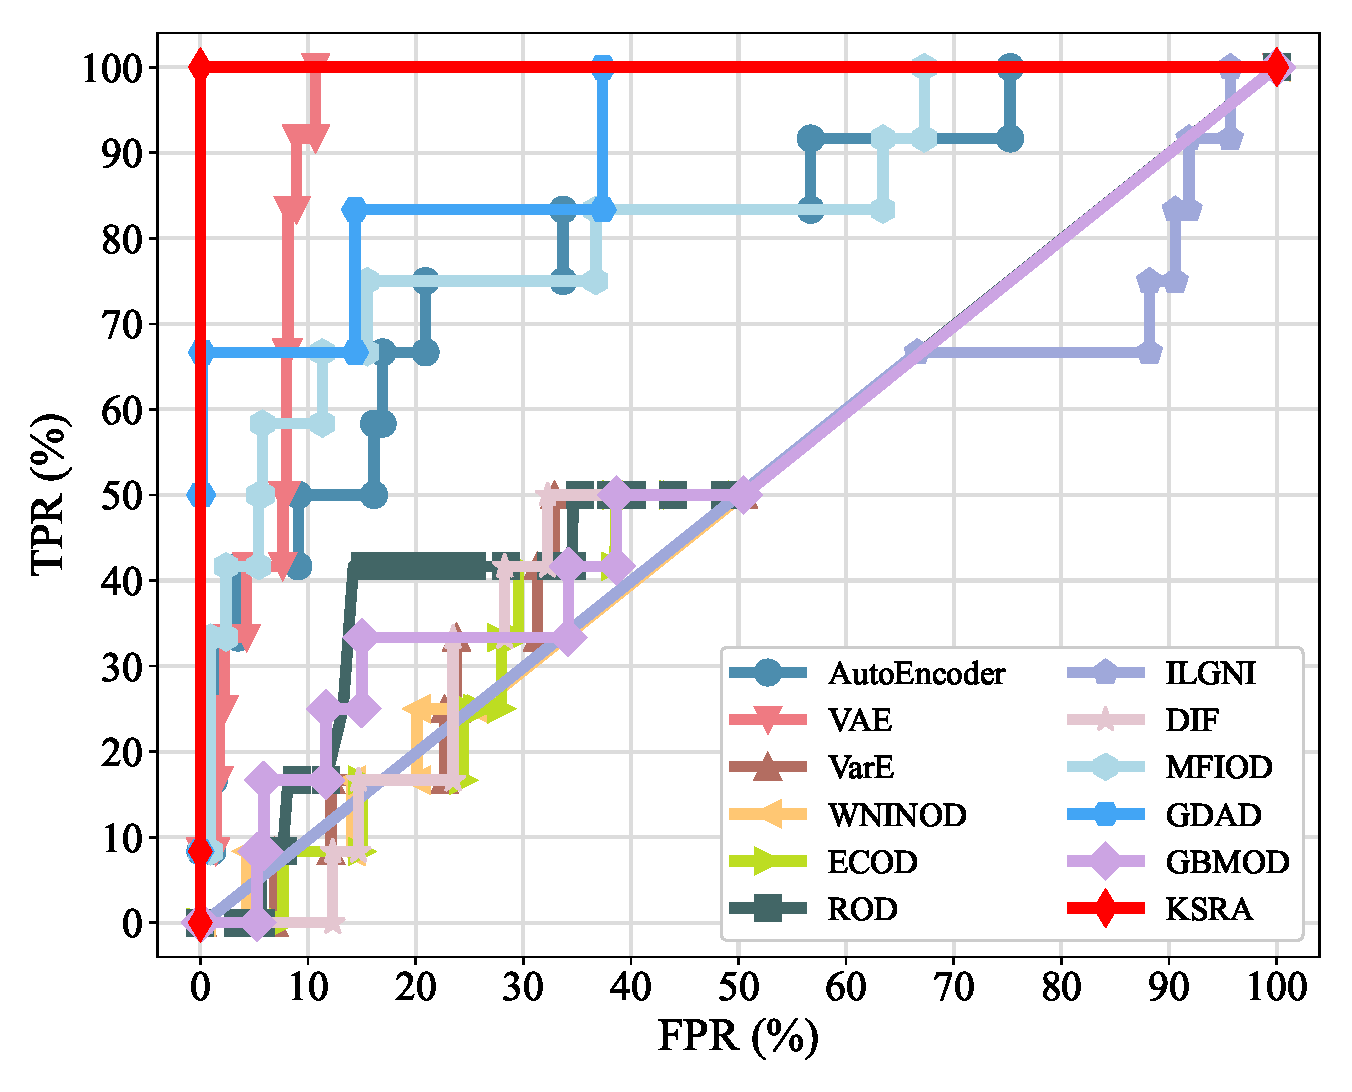
\includegraphics[width=\textwidth]{Figures/tic_tac_toe_negative_12_variant1_ROC.eps}
    \small (o) Tic\_12
    \label{fig:Tic_12}
  \end{minipage}
  \hfill
  \begin{minipage}[b]{0.24\textwidth}
    \centering
    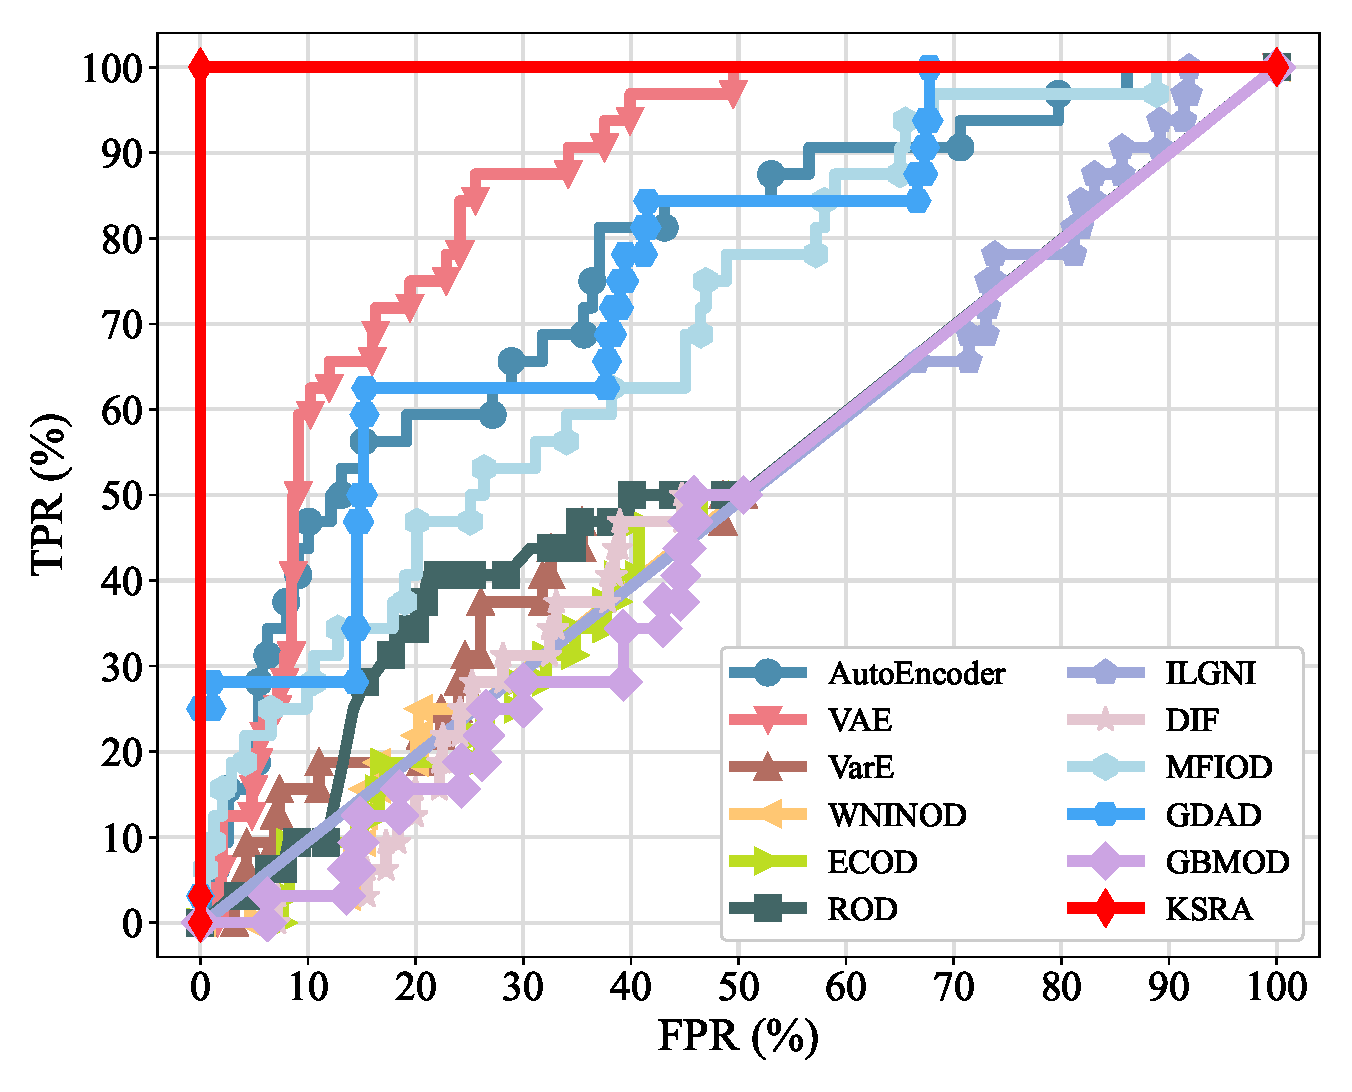
\includegraphics[width=\textwidth]{Figures/tic_tac_toe_negative_32_variant1_ROC.eps}
    \small (p) Tic\_32
    \label{fig:Tic_32}
  \end{minipage}

  \vspace{10pt}

  % =================== 第五行 (17-20) ===================
  \begin{minipage}[b]{0.24\textwidth}
    \centering
    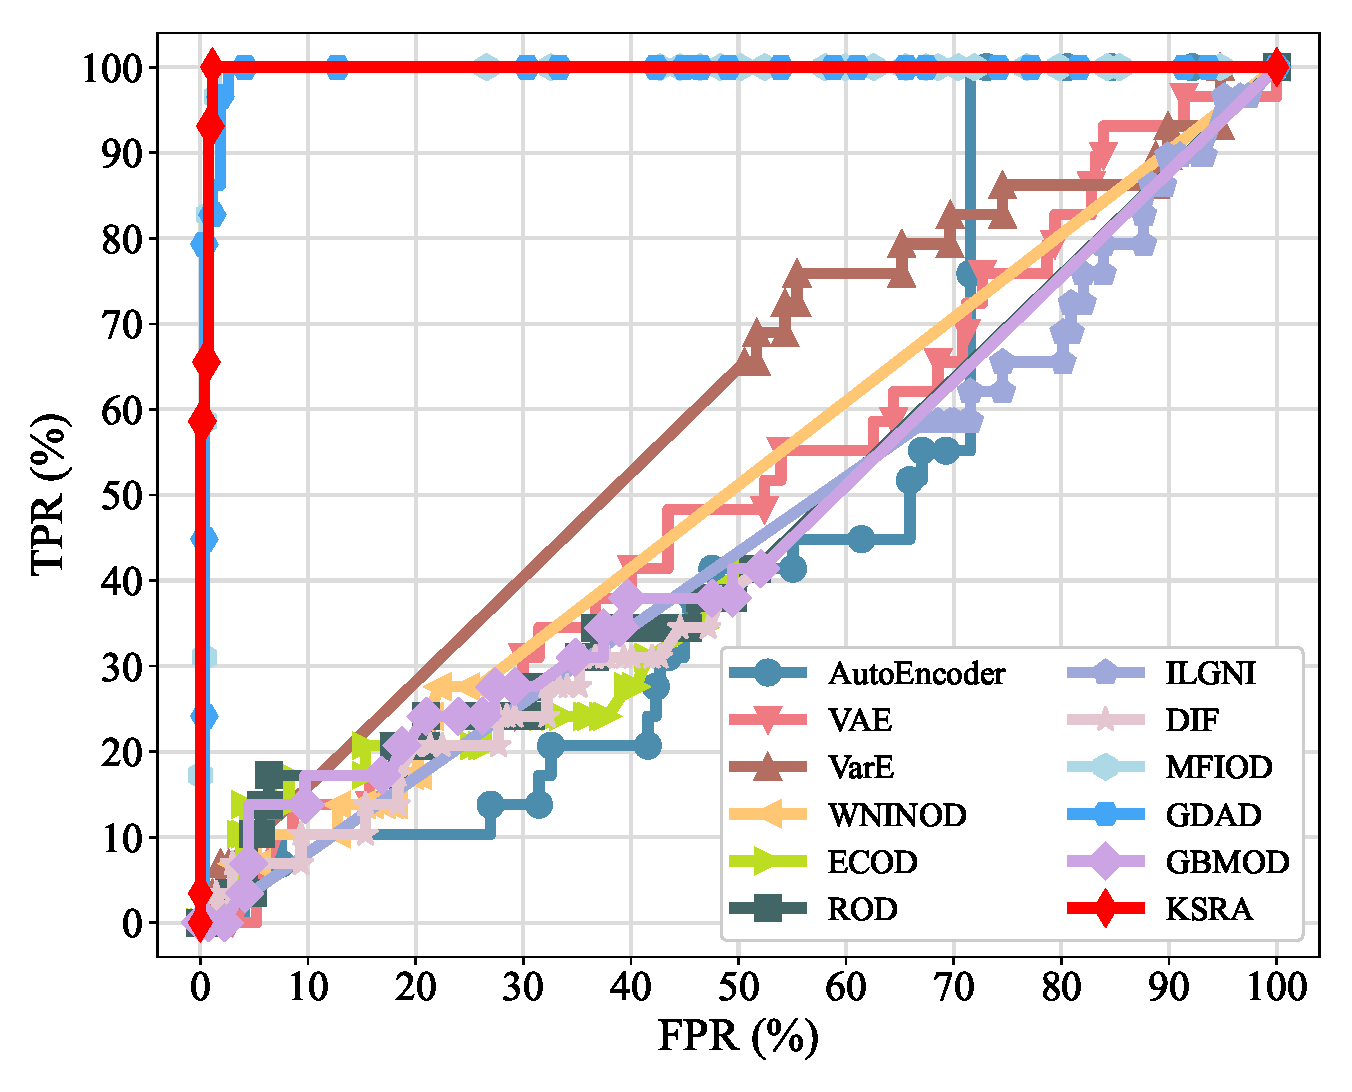
\includegraphics[width=\textwidth]{Figures/vote_republican_29_variant1_ROC.eps}
    \small (q) Vote
    \label{fig:Vote}
  \end{minipage}
  \hfill
  \begin{minipage}[b]{0.24\textwidth}
    \centering
    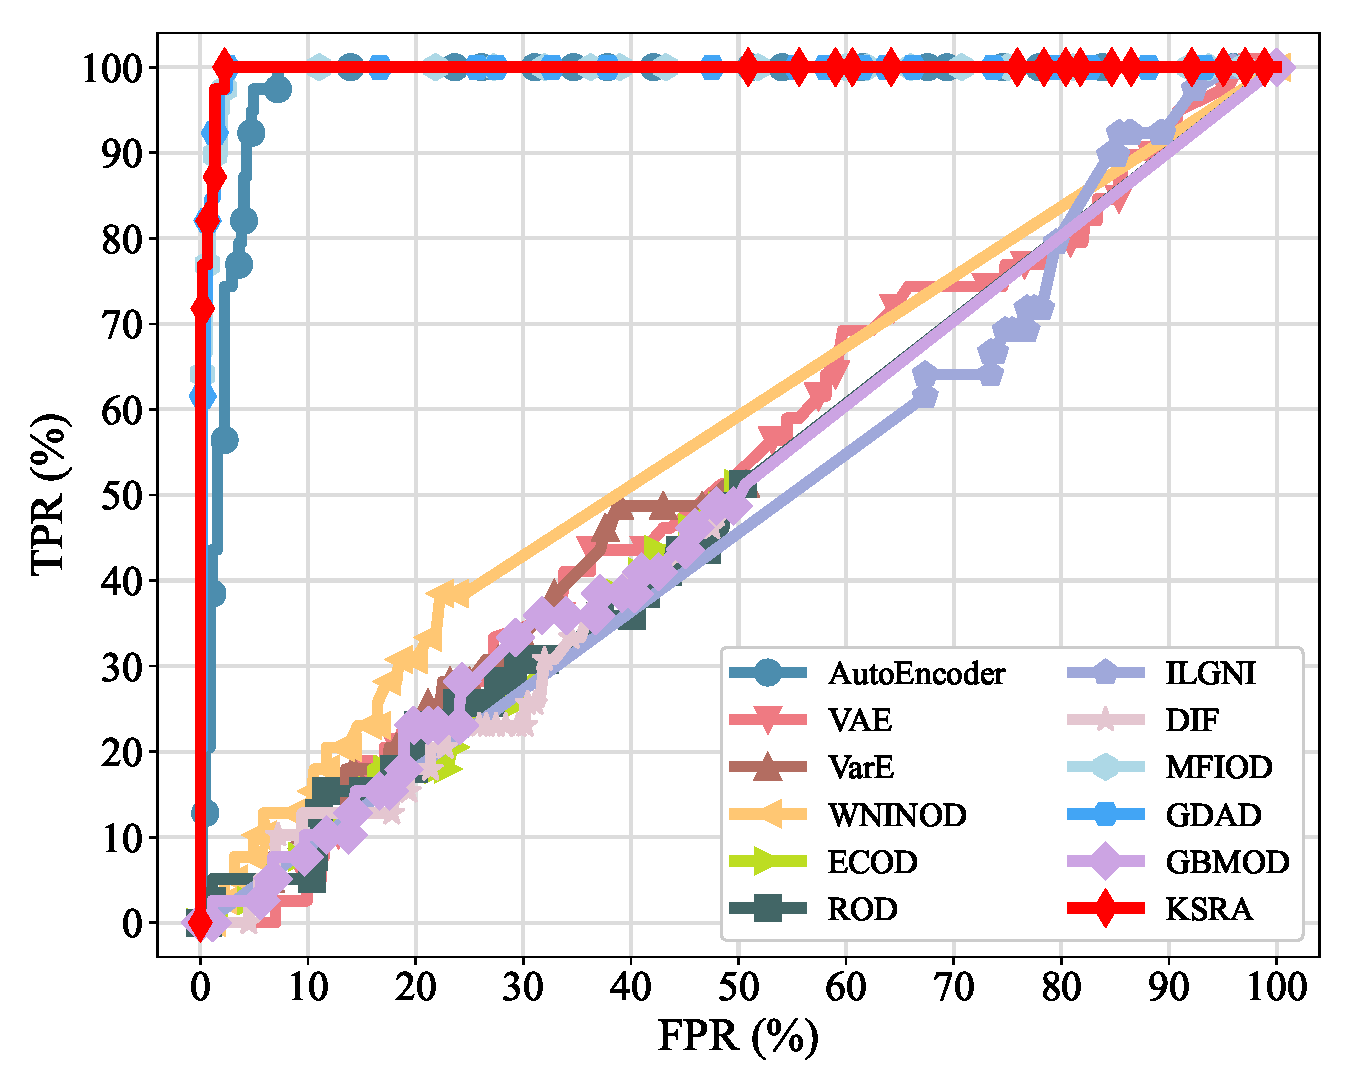
\includegraphics[width=\textwidth]{Figures/wbc_malignant_39_variant1_ROC.eps}
    \small (r) Wbc
    \label{fig:Wbc}
  \end{minipage}
  \hfill
  \begin{minipage}[b]{0.24\textwidth}
    \centering
    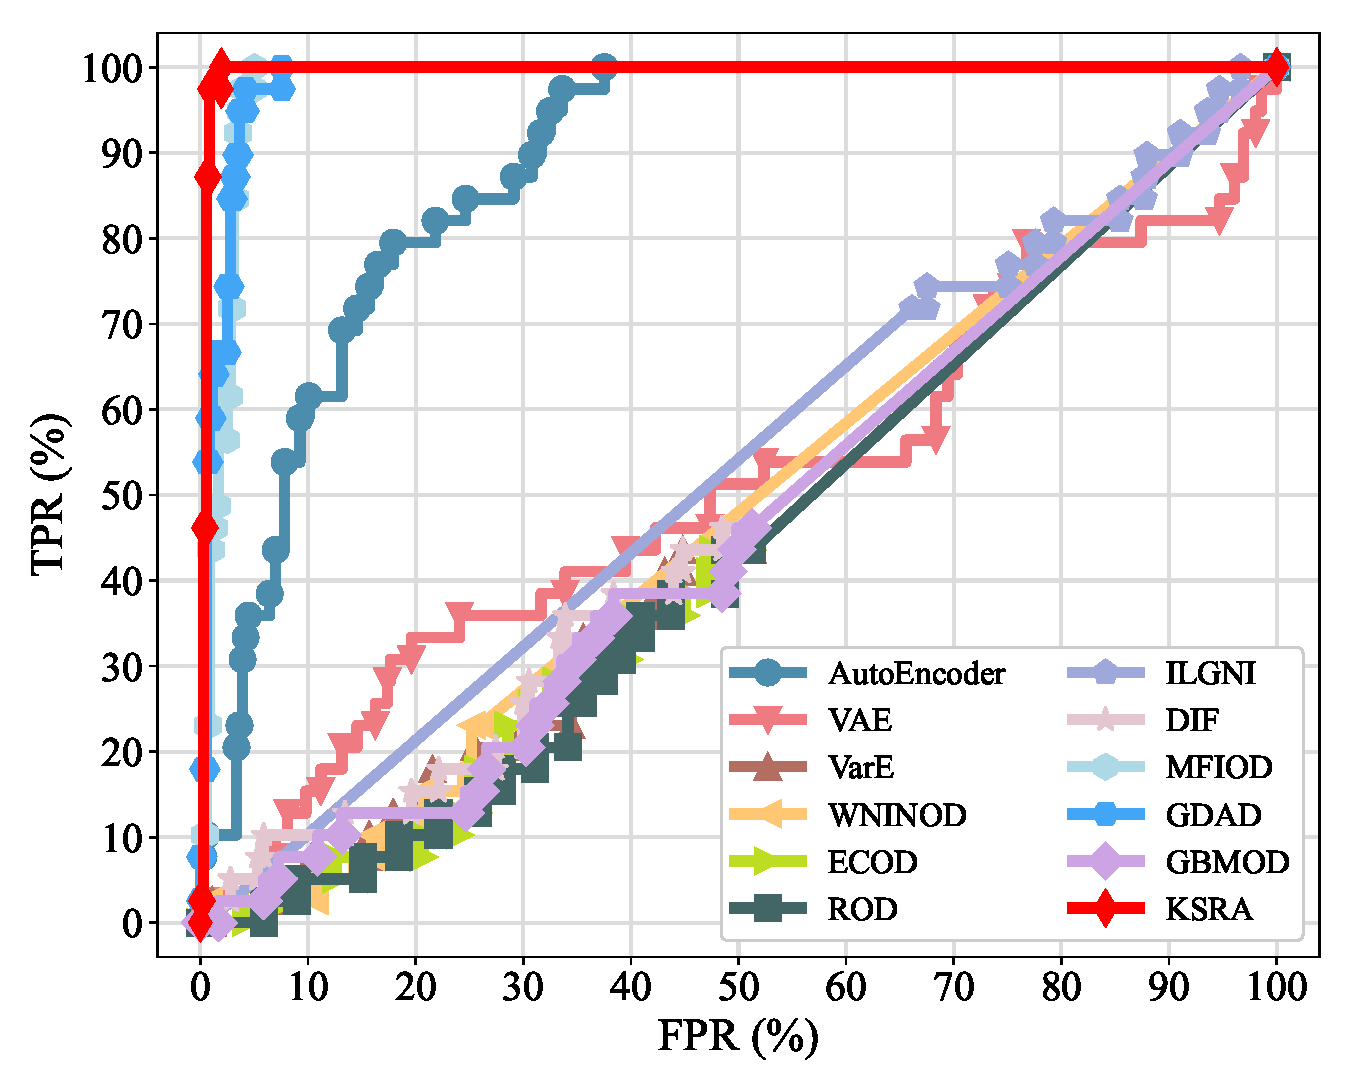
\includegraphics[width=\textwidth]{Figures/wdbc_M_39_variant1_ROC.eps}
    \small (s) Wdbc\_M
    \label{fig:Wdbc_M}
  \end{minipage}
  \hfill
  \begin{minipage}[b]{0.24\textwidth}
    \centering
    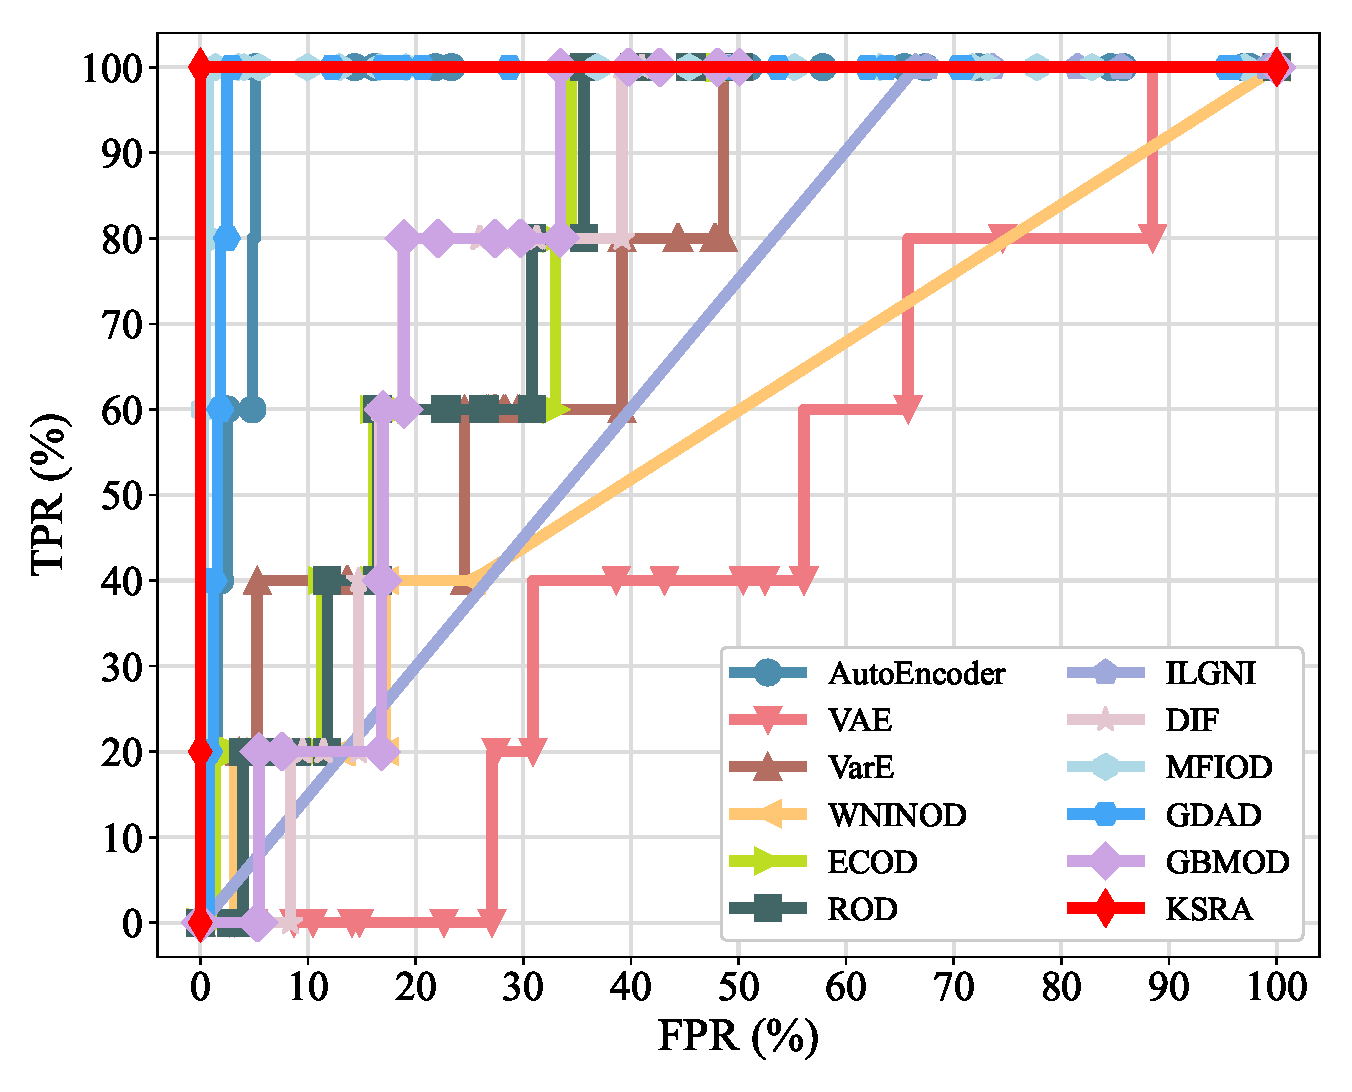
\includegraphics[width=\textwidth]{Figures/yeast_ERL_5_variant1_ROC.eps}
    \small (t) Yeast
    \label{fig:Yeast}
  \end{minipage}

  \vspace{10pt}
  \caption{ROC curves on 20 datasets.}\label{fig:all_rocs}
\end{figure*}

\begin{table*}[!ht]
	\centering
	\caption{Experimental comparison results. Runtime values are descriptive; complete original environment metadata and repeated-run timing statistics were not retained.}\label{KSRA-AUC}
	\resizebox{1\textwidth}{!}{
		\begin{tabular}{lccccccccccc|cccc|c}
            \toprule
            Datasets & AutoEncoder & VAE & VarE & WNINOD & ECOD & ROD & ILGNI & DIF & MFIOD & GDAD & GBMOD & KSRA$_1$ & KSRA$_2$ & KSRA$_3$ & KSRA$_4$ & KSRA$_{best}$ \\\midrule
            Annealing & 0.714 & 0.752 & 0.619 & 0.791 & 0.787 & 0.712 & 0.686 & 0.792 & 0.743 & 0.741 & 0.822 & \textbf{0.839} & 0.835 & \underline{0.836} & 0.828 & \textbf{0.839} \\
            Arrhythmia & 0.768 & 0.780 & 0.739 & 0.815 & 0.807 & 0.801 & 0.816 & 0.809 & 0.816 & 0.806 & 0.810 & \underline{0.820} & \textbf{0.821} & 0.819 & 0.778 & \textbf{0.821} \\
            Audio & 0.655 & 0.664 & 0.792 & 0.778 & 0.833 & 0.615 & 0.873 & 0.549 & 0.842 & 0.825 & 0.681 & 0.898 & \textbf{0.904} & \underline{0.902} & 0.824 & \textbf{0.904} \\
            Bands & 0.939 & 0.917 & 0.702 & 0.882 & 0.936 & 0.808 & 0.874 & 0.816 & 0.545 & 0.848 & \underline{0.948} & \textbf{0.948} & 0.927 & 0.924 & 0.942 & \textbf{0.948} \\
            Cardio & 0.884 & \textbf{0.952} & 0.526 & 0.949 & 0.935 & 0.932 & 0.887 & 0.918 & 0.834 & 0.918 & 0.925 & 0.948 & 0.948 & 0.946 & \underline{0.950} & \underline{0.950} \\
            Cardio\_33 & 0.848 & 0.843 & 0.780 & 0.851 & 0.871 & \underline{0.893} & 0.811 & 0.796 & 0.697 & 0.858 & 0.864 & 0.878 & 0.886 & \textbf{0.893} & 0.878 & \textbf{0.893} \\
            Chess\_16 & 0.939 & 0.920 & 0.956 & 0.975 & 0.969 & 0.972 & 0.950 & 0.877 & 0.961 & 0.951 & 0.973 & 0.973 & \textbf{0.977} & \underline{0.977} & 0.969 & \textbf{0.977} \\
            Chess\_34 & 0.959 & 0.943 & 0.892 & 0.964 & 0.968 & 0.954 & 0.935 & 0.830 & 0.957 & 0.863 & \textbf{0.969} & 0.963 & 0.968 & \underline{0.969} & 0.937 & \underline{0.969} \\
            Ecoli & 0.909 & 0.812 & 0.899 & 0.874 & 0.781 & 0.613 & 0.638 & 0.864 & 0.835 & 0.635 & 0.918 & 0.950 & \textbf{0.964} & \underline{0.957} & 0.952 & \textbf{0.964} \\
            Iris & 0.962 & 0.663 & 1.000 & 1.000 & 0.977 & 0.866 & 0.951 & 0.779 & 0.999 & 0.997 & \underline{1.000} & \textbf{1.000} & 0.999 & 0.999 & 0.998 & \textbf{1.000} \\
            Lymphography & 0.982 & 0.999 & 0.507 & 0.992 & 0.996 & 0.762 & 0.991 & 0.982 & 0.986 & 0.993 & 0.998 & 0.992 & 0.998 & \underline{0.999} & \textbf{1.000} & \textbf{1.000} \\
            Monks & 0.952 & 0.939 & 0.727 & 0.978 & 0.987 & 0.968 & 1.000 & 0.912 & 0.987 & 1.000 & 0.917 & \underline{1.000} & \textbf{1.000} & 0.991 & 0.998 & \textbf{1.000} \\
            Mushroom & 0.821 & 0.888 & 0.880 & 0.912 & 0.949 & 0.847 & 0.961 & 0.847 & 0.940 & \textbf{0.970} & 0.916 & \underline{0.969} & 0.954 & 0.957 & 0.945 & \underline{0.969} \\
            Sick & 0.837 & 0.795 & 0.691 & 0.754 & 0.843 & \textbf{0.895} & 0.807 & 0.797 & 0.778 & \underline{0.851} & 0.833 & 0.796 & 0.848 & 0.850 & 0.829 & 0.850 \\
            Tic\_12 & 0.937 & 0.813 & 0.733 & 0.967 & 0.948 & 0.900 & 0.813 & 0.829 & 0.824 & 0.913 & 0.989 & 0.915 & \underline{1.000} & \textbf{1.000} & 0.983 & \textbf{1.000} \\
            Tic\_32 & 0.859 & 0.785 & 0.563 & 0.894 & 0.878 & 0.749 & 0.722 & 0.801 & 0.695 & 0.758 & 0.917 & 0.758 & \underline{1.000} & \textbf{1.000} & 0.929 & \textbf{1.000} \\
            Vote & 0.994 & 0.995 & 0.981 & 0.995 & 0.995 & 0.995 & 0.994 & 0.801 & 0.996 & 0.994 & 0.997 & \textbf{0.997} & \underline{0.997} & 0.997 & 0.968 & \textbf{0.997} \\
            Wbc & 0.994 & 0.992 & \textbf{0.997} & \underline{0.997} & 0.995 & 0.985 & 0.988 & 0.939 & 0.995 & 0.995 & 0.997 & 0.997 & 0.997 & 0.997 & 0.997 & 0.997 \\
            Wdbc\_M & 0.965 & 0.986 & \textbf{0.997} & \underline{0.996} & 0.959 & 0.995 & 0.951 & 0.871 & 0.981 & 0.985 & 0.996 & 0.995 & 0.995 & 0.995 & 0.995 & 0.995 \\
            Yeast & 0.995 & 0.995 & 1.000 & 0.998 & 0.995 & 0.949 & 0.981 & 0.987 & 0.996 & 0.984 & 1.000 & 1.000 & 1.000 & \underline{1.000} & \textbf{1.000} & \textbf{1.000} \\
            \midrule
            Average AUC & 0.896 & 0.872 & 0.、。；799 & 0.918 & 0.921 & 0.861 & 0.881 & 0.840 & 0.870 & 0.894 & \underline{0.923} & 0.932 & 0.951 & 0.950 & 0.935 & \textbf{0.954} \\
            Average Runtime(s) & 2.137 & 5.811 & 3.408 & 35.353 & 0.057 & 1527.336 & 184.858 & 1.741 & 0.785 & 0.790 & 2.435 & 26.757 & 0.724 & 12.103 & 41.968 & - \\
            \bottomrule
        \end{tabular}}
\end{table*}

\begin{table*}[!ht]
    \centering
    \caption{AUC comparison of KSRA with additional baseline methods.}\label{tab:additional_baselines}
    \resizebox{0.8\textwidth}{!}{
        \begin{tabular}{lcccc|cccc|c}
            \toprule
            Datasets & DVGAE-GAN & Kernel PCA & LRR & OCSVM-RBF & KSRA$_1$ & KSRA$_2$ & KSRA$_3$ & KSRA$_4$ & KSRA$_{best}$ \\
            \midrule
            Annealing & 0.754 & 0.776 & 0.751 & 0.743 & \textbf{0.839} & 0.835 & \underline{0.836} & 0.828 & \textbf{0.839} \\
            Arrhythmia & 0.785 & 0.782 & 0.787 & 0.758 & \underline{0.820} & \textbf{0.821} & 0.819 & 0.778 & \textbf{0.821} \\
            Audio & 0.868 & 0.828 & 0.900 & 0.809 & 0.898 & \textbf{0.904} & \underline{0.902} & 0.824 & \textbf{0.904} \\
            Bands & 0.882 & \textbf{0.952} & 0.887 & \textbf{0.952} & \underline{0.948} & 0.927 & 0.924 & 0.942 & \underline{0.948} \\
            Cardio & 0.892 & 0.941 & \underline{0.949} & 0.912 & 0.948 & 0.948 & 0.946 & \textbf{0.950} & \textbf{0.950} \\
            Cardio\_33 & 0.839 & 0.856 & 0.845 & \underline{0.889} & 0.878 & 0.886 & \textbf{0.893} & 0.878 & \textbf{0.893} \\
            Chess\_16 & 0.970 & \textbf{0.996} & 0.971 & \underline{0.990} & 0.973 & 0.977 & 0.977 & 0.969 & 0.977 \\
            Chess\_34 & 0.969 & \textbf{0.992} & 0.959 & \underline{0.984} & 0.963 & 0.968 & 0.969 & 0.937 & 0.969 \\
            Ecoli & 0.856 & 0.889 & 0.897 & 0.931 & 0.950 & \textbf{0.964} & \underline{0.957} & 0.952 & \textbf{0.964} \\
            Iris & 0.850 & 0.959 & 0.627 & \textbf{1.000} & \textbf{1.000} & \underline{0.999} & \underline{0.999} & 0.998 & \textbf{1.000} \\
            Lymphography & 0.991 & \textbf{1.000} & 0.998 & \textbf{1.000} & 0.992 & 0.998 & \underline{0.999} & \textbf{1.000} & \textbf{1.000} \\
            Monks & 0.764 & \textbf{1.000} & 0.987 & \textbf{1.000} & \textbf{1.000} & \textbf{1.000} & 0.991 & \underline{0.998} & \textbf{1.000} \\
            Mushroom & 0.973 & \textbf{0.979} & 0.975 & \underline{0.979} & 0.969 & 0.954 & 0.957 & 0.945 & 0.969 \\
            Sick & 0.794 & 0.835 & 0.770 & 0.847 & 0.796 & \underline{0.848} & \textbf{0.850} & 0.829 & \textbf{0.850} \\
            Tic\_12 & 0.855 & \textbf{1.000} & \textbf{1.000} & \textbf{1.000} & 0.915 & \textbf{1.000} & \textbf{1.000} & \underline{0.983} & \textbf{1.000} \\
            Tic\_32 & 0.770 & \textbf{1.000} & \textbf{1.000} & \textbf{1.000} & 0.758 & \textbf{1.000} & \textbf{1.000} & \underline{0.929} & \textbf{1.000} \\
            Vote & 0.325 & 0.650 & 0.995 & 0.994 & \textbf{0.997} & \underline{0.997} & \underline{0.997} & 0.968 & \textbf{0.997} \\
            Wbc & 0.972 & 0.990 & 0.814 & 0.996 & \textbf{0.997} & \underline{0.997} & \textbf{0.997} & \underline{0.997} & \textbf{0.997} \\
            Wdbc\_M & 0.805 & 0.971 & 0.883 & 0.989 & \underline{0.995} & \textbf{0.995} & \underline{0.995} & 0.995 & \textbf{0.995} \\
            Yeast & 0.996 & \underline{0.999} & 0.995 & \textbf{1.000} & \textbf{1.000} & \textbf{1.000} & \textbf{1.000} & \textbf{1.000} & \textbf{1.000} \\
            \midrule
            Average AUC & 0.845 & 0.920 & 0.900 & 0.939 & 0.932 & \underline{0.951} & 0.950 & 0.935 & \textbf{0.954} \\
            \bottomrule
        \end{tabular}}
\end{table*}

\subsection{Evaluation Using Average Precision}

To complement ROC-AUC, particularly for datasets with low anomaly ratios, we additionally report average precision (AP) across the 20 benchmark datasets. Treating anomalies as the positive class, AP summarizes precision at different recall levels:
\begin{equation*}\label{AP_equ}
    \mathrm{AP}=\sum_{k=1}^{K}(R_k-R_{k-1})P_k,
\end{equation*}
where $P_k$ and $R_k$ denote precision and recall at the $k$-th score threshold, respectively, and $R_0=0$. Higher AP indicates a better balance between retrieving anomalies and limiting false positives. We use non-interpolated AP rather than trapezoidal PR-AUC.
AP is calculated directly from archived per-sample anomaly scores, retaining the existing configurations and score directions without parameter reselection using AP. The comparison includes 15 baseline methods and four KSRA variants. The KSRA$_{best}$ column reports the AP of the variant previously selected by the highest test ROC-AUC on each dataset. It is therefore an oracle-selected reference rather than the maximum AP across variants. Anomaly ratios are included in the table, and overall performance is summarized by the unweighted mean AP across datasets. Excluding KSRA$_{best}$, the best and second-best results are shown in bold and underlined, respectively, with ties retained.

The results are shown in Table \ref{tab:ap_comparison}, which indicates that KSRA remains competitive under AP evaluation, although its advantages vary across datasets and variants.
\begin{enumerate}
    \item The four KSRA variants achieve mean AP values of 0.6092, 0.6764, 0.6639, and 0.6107, respectively. The variant KSRA$_2$ obtains the highest mean AP, indicating that its overall advantage extends beyond ROC-AUC to anomaly class precision–recall performance.

    \item OCSVM-RBF is the strongest baseline in mean AP, achieving 0.6637. The variant KSRA$_2$ exceeds it by approximately 1.28 percentage points, whereas KSRA$_3$ achieves a similar result. Strong baselines therefore remain competitive under AP evaluation.
    
    \item KSRA$_{best}$ achieves a mean AP of 0.6675, below that of KSRA$_2$. Thus, selecting variants by ROC-AUC does not necessarily yield higher AP, illustrating the complementary information provided by the two metrics.
\end{enumerate}

\begin{table*}[!ht]
    \centering
    \caption{Average precision comparison across 20 benchmark datasets.}\label{tab:ap_comparison}
    \resizebox{1\textwidth}{!}{
        \begin{tabular}{lcccccccccccccccc|cccc|c}
            \toprule
            Datasets & Anomaly ratio (\%) & AutoEncoder & VAE & VarE & WNINOD & ECOD & ROD & ILGNI & DIF & MFIOD & GDAD & GBMOD & DVGAE-GAN & Kernel PCA & LRR & OCSVM-RBF & KSRA$_1$ & KSRA$_2$ & KSRA$_3$ & KSRA$_4$ & KSRA$_{best}$ \\
            \midrule
            Annealing & 5.26 & 0.095 & 0.100 & 0.147 & 0.226 & 0.203 & 0.112 & 0.093 & 0.120 & 0.156 & 0.129 & 0.267 & 0.123 & 0.165 & 0.115 & 0.127 & \textbf{0.289} & \underline{0.282} & 0.277 & 0.265 & 0.289 \\
            Arrhythmia & 14.60 & 0.356 & 0.399 & 0.288 & 0.488 & 0.465 & \textbf{0.514} & \underline{0.494} & 0.457 & 0.404 & 0.480 & 0.468 & 0.448 & 0.430 & 0.454 & 0.421 & 0.472 & 0.474 & 0.472 & 0.442 & 0.474 \\
            Audio & 25.22 & 0.474 & 0.490 & 0.516 & 0.546 & 0.654 & 0.371 & 0.691 & 0.311 & 0.650 & 0.681 & 0.459 & 0.666 & 0.689 & 0.736 & 0.604 & 0.736 & \textbf{0.746} & \underline{0.743} & 0.628 & 0.746 \\
            Bands & 1.89 & 0.155 & 0.128 & 0.050 & 0.158 & \underline{0.423} & 0.107 & 0.284 & 0.153 & 0.190 & 0.080 & 0.182 & 0.136 & 0.321 & 0.266 & \textbf{0.425} & 0.246 & 0.420 & 0.354 & 0.262 & 0.246 \\
            Cardio & 9.61 & 0.304 & \textbf{0.701} & 0.105 & 0.645 & 0.567 & 0.554 & 0.439 & 0.551 & 0.424 & 0.494 & 0.577 & 0.516 & 0.632 & \underline{0.692} & 0.566 & 0.649 & 0.650 & 0.646 & 0.668 & 0.668 \\
            Cardio\_33 & 1.95 & 0.047 & 0.113 & 0.057 & 0.109 & 0.153 & 0.122 & 0.062 & 0.081 & 0.049 & 0.090 & \underline{0.154} & 0.128 & 0.118 & 0.094 & \textbf{0.156} & 0.147 & 0.149 & 0.129 & 0.138 & 0.129 \\
            Chess\_16 & 0.95 & 0.106 & 0.056 & 0.116 & 0.155 & 0.128 & 0.147 & 0.090 & 0.210 & 0.111 & 0.176 & 0.217 & 0.140 & \textbf{0.554} & 0.140 & \underline{0.360} & 0.148 & 0.168 & 0.167 & 0.165 & 0.168 \\
            Chess\_34 & 2.00 & 0.335 & 0.252 & 0.109 & 0.211 & 0.234 & 0.178 & 0.137 & 0.331 & 0.206 & 0.137 & 0.291 & 0.270 & \textbf{0.620} & 0.188 & \underline{0.443} & 0.203 & 0.233 & 0.239 & 0.273 & 0.239 \\
            Ecoli & 2.68 & 0.576 & 0.651 & 0.336 & 0.626 & 0.187 & 0.052 & 0.041 & 0.471 & 0.450 & 0.048 & 0.644 & 0.359 & 0.316 & \textbf{0.763} & 0.636 & 0.676 & 0.682 & 0.672 & \underline{0.684} & 0.682 \\
            Iris & 9.91 & 0.287 & 0.776 & \textbf{1.000} & \textbf{1.000} & 0.713 & 0.429 & 0.531 & 0.200 & \underline{0.992} & 0.978 & \textbf{1.000} & 0.611 & 0.575 & 0.131 & \textbf{1.000} & \textbf{1.000} & \underline{0.992} & \underline{0.992} & 0.986 & 1.000 \\
            Lymphography & 4.05 & 0.719 & 0.852 & 0.095 & 0.863 & 0.915 & 0.277 & 0.882 & 0.734 & 0.802 & 0.896 & 0.958 & 0.859 & \textbf{1.000} & 0.958 & \textbf{1.000} & 0.889 & 0.948 & \underline{0.976} & \textbf{1.000} & 1.000 \\
            Monks & 1.72 & 0.111 & 0.790 & 0.153 & 0.631 & 0.812 & 0.239 & \textbf{1.000} & 0.122 & 0.812 & \textbf{1.000} & 0.514 & 0.225 & \textbf{1.000} & 0.812 & \textbf{1.000} & \textbf{1.000} & \textbf{1.000} & 0.833 & \underline{0.917} & 1.000 \\
            Mushroom & 4.99 & 0.287 & 0.289 & 0.401 & 0.414 & 0.486 & 0.382 & 0.888 & 0.366 & 0.426 & 0.899 & 0.401 & \underline{0.900} & 0.891 & \textbf{0.901} & 0.681 & 0.807 & 0.888 & 0.892 & 0.870 & 0.807 \\
            Sick & 1.99 & 0.061 & 0.062 & 0.032 & 0.038 & 0.066 & \textbf{0.180} & 0.055 & 0.062 & 0.046 & 0.078 & 0.071 & 0.064 & 0.070 & 0.050 & \underline{0.088} & 0.044 & 0.059 & 0.060 & 0.054 & 0.060 \\
            Tic\_12 & 1.88 & 0.201 & 0.210 & 0.036 & 0.348 & 0.210 & 0.107 & 0.162 & 0.061 & 0.236 & 0.671 & 0.503 & 0.185 & \textbf{1.000} & \textbf{1.000} & \textbf{1.000} & \underline{0.691} & \textbf{1.000} & \textbf{1.000} & 0.637 & 1.000 \\
            Tic\_32 & 4.86 & 0.154 & 0.164 & 0.056 & 0.209 & 0.171 & 0.118 & 0.120 & 0.133 & 0.158 & 0.345 & 0.284 & 0.168 & \textbf{1.000} & \textbf{1.000} & \textbf{1.000} & 0.346 & \textbf{1.000} & \textbf{1.000} & \underline{0.598} & 1.000 \\
            Vote & 9.80 & 0.098 & 0.923 & 0.754 & 0.914 & 0.923 & 0.953 & 0.880 & 0.321 & 0.942 & 0.911 & \underline{0.965} & 0.070 & 0.140 & 0.930 & 0.947 & \textbf{0.968} & 0.964 & 0.965 & 0.762 & 0.968 \\
            Wbc & 8.07 & 0.726 & 0.855 & \textbf{0.970} & 0.967 & 0.946 & 0.825 & 0.889 & 0.412 & 0.943 & 0.930 & 0.965 & 0.721 & 0.869 & 0.179 & 0.963 & 0.967 & 0.967 & \underline{0.968} & 0.967 & 0.967 \\
            Wdbc\_M & 9.85 & 0.387 & 0.623 & \textbf{0.951} & \underline{0.920} & 0.543 & 0.894 & 0.675 & 0.298 & 0.755 & 0.832 & 0.915 & 0.344 & 0.685 & 0.432 & 0.857 & 0.904 & 0.906 & 0.892 & 0.900 & 0.906 \\
            Yeast & 0.44 & 0.091 & 0.288 & \textbf{1.000} & 0.563 & 0.358 & 0.055 & 0.152 & 0.159 & 0.396 & 0.136 & \textbf{1.000} & 0.364 & \underline{0.877} & 0.316 & \textbf{1.000} & \textbf{1.000} & \textbf{1.000} & \textbf{1.000} & \textbf{1.000} & 1.000 \\
            \midrule
            Average AP & -- & 0.279 & 0.436 & 0.359 & 0.501 & 0.458 & 0.331 & 0.428 & 0.278 & 0.457 & 0.500 & 0.542 & 0.365 & 0.598 & 0.508 & 0.664 & 0.609 & \textbf{0.676} & \underline{0.664} & 0.611 & 0.667 \\
            \bottomrule
        \end{tabular}}
\end{table*}


\subsection{Variant Analysis}\label{Variant Analysis}

This subsection provides a detailed analysis of the performance of four variants of our model across 20 datasets.
The right part of Table \ref{KSRA-AUC} presents the specific AUC values and average runtime experimental results for the variants. In particular, KSRA$_1$ represents the result obtained from Equation (\ref{Case1}) in the self-representation section; KSRA$_2$ denotes the results obtained from Eq.~(\ref{Case2}); KSRA$_3$ denotes the results obtained from Eq.~(\ref{Case3}), and KSRA$_4$ corresponds to Eq.~(\ref{Case4}). The table indicates that KSRA$_2$, using F-norm for loss and regularization, excels in both mean AUC and running time. Although KSRA$_3$ delivers a similar AUC performance, its average running time is slightly inferior. Therefore, KSRA$_2$ demonstrates superior performance compared to the other three variants.

This observation differs from the common expectation that sparsity-promoting $\ell_{2,1}$ regularization necessarily yields superior anomaly detection performance. A possible explanation is that the similarity-profile representation already captures useful nonlinear relationships, making coefficient shrinkage preferable to stronger sparsity in some datasets. Under this setting, preserving global sample relationships becomes more beneficial than aggressively enforcing sparsity. The Frobenius norm preserves dense collaborative relationships among samples, allowing richer structural information to be propagated during the subsequent random walk stage. Excessive sparsity may inadvertently remove weak yet informative connections that contribute to global anomaly characterization. From an optimization perspective, KSRA$_2$ admits a closed-form solution and avoids iterative reweighting procedures, leading to substantially lower computational cost.


\subsection{Statistical Analysis}

Based on recent studies \cite{cheng2025gbmod,su2025identifying,su2025granular} on anomaly detection, we employed the non-parametric Friedman test supplemented by the Nemenyi post-hoc test to verify whether the performance improvement of our proposed KSRA method is statistically significant. This approach compares method ranks across datasets without assuming normally distributed AUC values. The Friedman test first confirms whether any overall differences exist among all methods, while the Nemenyi test further determines whether the performance gaps between algorithms significantly exceed the range of statistical random fluctuations. Throughout this analysis, KSRA denotes the fixed Frobenius norm variant, implemented as KSRA$_2$.

For the AUC metric, we can obtain the $F$ distribution with degrees of freedom 11 and 209 using Friedman's test. At the pre-specified significance level $\alpha=0.05$, the test statistic $\tau_F=12.13$ far exceeds the critical value of 1.83. The results indicate that these evaluation methods exhibit statistically significant differences in performance. Therefore, it is necessary to conduct the Nemenyi post-hoc test to further distinguish the specific performance among the various methods.

The Nemenyi test figure plotted based on the results is shown in Fig.\ref{fig:CD_diagram}. The figure displays the critical difference $CD=3.7261$ at a significance level of $\alpha = 0.05$. The horizontal axis at the top of the figure represents the average rank of all evaluated methods across all datasets. Each method's position on the axes corresponds to its average rank. If two or more algorithms are connected by a horizontal red line segment, it indicates that the performance difference between them is not statistically significant. Conversely, if no line segment connects two algorithms, it signifies that they exhibit a statistically significant difference at the $\alpha = 0.05$ level.

\begin{enumerate}[\indent (1)]
    \item Our KSRA method occupies the far left position on the axis, significantly outperforming AutoEncoder, VAE, VarE, ROD, ILGNI, DIF, MFIOD, and GDAD in overall performance.
    \item Although our method overlaps with GBMOD, WNINOD and ECOD along the red line, this merely indicates that their differences are not sufficiently extreme at the current sample size.
    \item Nevertheless, its leading position in the ranking still demonstrates its relatively favorable average rank under the current evaluation scheme.
\end{enumerate}

To complement the overall rank-based comparisons, we additionally conduct two-sided Wilcoxon signed-rank tests between KSRA and each baseline, applying Holm correction across all 11 comparisons to control the family-wise error rate. Table \ref{tab:wilcoxon_holm} summarizes the mean and median AUC differences, win/tie/loss counts, and raw and adjusted $p-$values. AUC differences are calculated as the AUC of KSRA minus that of the corresponding baseline; positive values favor KSRA. Win/tie/loss counts describe numerical outcomes rather than dataset-level significance. To match the precision of the supplied baseline AUC, paired differences are rounded to nine decimal places for testing and counting. Zero differences are excluded, tied absolute differences receive average ranks, and two-sided $p-$values are calculated from the exact sign-permutation distribution.

\begin{enumerate}[\indent (1)]
    \item KSRA exhibits positive mean AUC differences against all 11 baselines, and all paired comparisons remain significant after Holm correction at $\alpha=0.05$.

    \item Against GBMOD, WNINOD, and ECOD, KSRA achieves win/tie/loss counts of 13/3/4, 16/0/4, and 18/1/1, with adjusted $p$-values of 0.004639, 0.000410, and 0.000410, respectively.
\end{enumerate}

Taken together, the Friedman test confirms overall performance
differences among the evaluated methods, while the Nemenyi test
places KSRA first in average rank without establishing significant differences from GBMOD, WNINOD, or ECOD. The supplementary Wilcoxon-Holm analysis detects significant paired differences favoring KSRA against all 11 baselines. 

\begin{figure*}
    \centering
    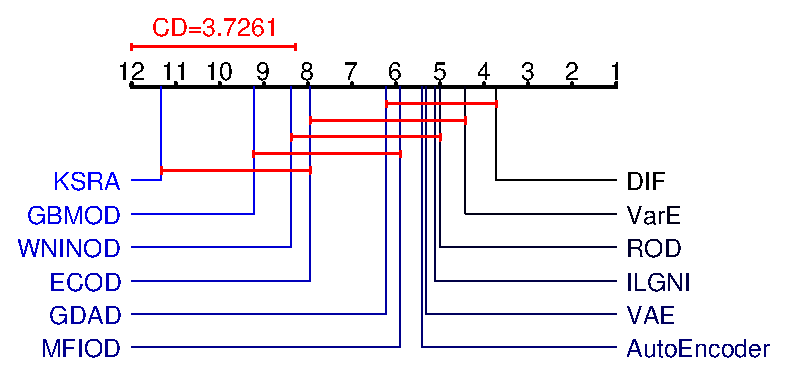
\includegraphics[scale=0.75]{Figures/NemenyiTestFig.eps}
    \caption{Nemenyi test figure on AUC.}
    \label{fig:CD_diagram}
\end{figure*}

\begin{table*}[!ht]
	\centering
	\caption{Pairwise AUC comparisons between KSRA and baseline methods using Wilcoxon signed-rank tests with Holm correction.}\label{tab:wilcoxon_holm}
	\resizebox{0.8\textwidth}{!}{
        \begin{tabular}{lcccccc}
            \hline
            Baseline & Mean $\Delta$AUC & Median $\Delta$AUC & W/T/L & $p$ & $p_{\mathrm{Holm}}$ & Sig. \\
            \hline
            AutoEncoder & +0.055256 & +0.037958 & 19/0/1 & 2.67029e-05 & 0.00018692 & Yes \\
            VAE & +0.079254 & +0.047604 & 18/0/2 & 1.33514e-05 & 0.000120163 & Yes \\
            VarE & +0.151784 & +0.094160 & 16/1/3 & 5.34058e-05 & 0.000320435 & Yes \\
            WNINOD & +0.032733 & +0.014184 & 16/0/4 & 8.2016e-05 & 0.00041008 & Yes \\
            ECOD & +0.030362 & +0.012927 & 18/1/1 & 9.53674e-05 & 0.00041008 & Yes \\
            ROD & +0.090352 & +0.041339 & 18/0/2 & 0.000209808 & 0.000629425 & Yes \\
            ILGNI & +0.069457 & +0.037362 & 18/1/1 & 1.90735e-05 & 0.000152588 & Yes \\
            DIF & +0.111025 & +0.100148 & 20/0/0 & 1.90735e-06 & 2.09808e-05 & Yes \\
            MFIOD & +0.080558 & +0.015491 & 19/1/0 & 3.8147e-06 & 3.8147e-05 & Yes \\
            GDAD & +0.056573 & +0.020973 & 17/1/2 & 0.000335693 & 0.000671387 & Yes \\
            GBMOD & +0.027394 & +0.011063 & 13/3/4 & 0.00463867 & 0.00463867 & Yes \\
            \hline
        \end{tabular}
    }
\end{table*}

\subsection{Hyper-parameter Sensitivity Analysis}

To examine the effects of hyperparameters, we evaluate the fixed KSRA$_2$ on 20 benchmark datasets by varying the regularization parameter $\lambda$, restart weight $d$, and kernel bandwidth $\sigma$ separately. We vary $\lambda$ over $\{10^{-8},10^{-7},\ldots,10^7\}$ while fixing $\sigma=\sigma_0$ and $d=0.85$, and $d$ over $\{0.05,0.10,0.15,0.30,0.50,0.70,0.85,0.95\}$ with
$\lambda=0.01$ and $\sigma=\sigma_0$. For bandwidth sensitivity, we set $\sigma=\alpha\sigma_0$, where
$\alpha\in\{0.25,0.5,0.75,1,1.25,1.5,2,4\}$, and fix
$\lambda=0.01$ and $d=0.85$. Here, $\sigma_0$ denotes the
mean off-diagonal mixed distance for each dataset. Fig.\ref{fig:parameters_sensitivity} presents the results, with ten datasets shown in each panel.

Overall, $\lambda$ and the kernel bandwidth substantially affect performance on some datasets, whereas the influence of $d$ is comparatively modest. The heterogeneous responses indicate that parameter selection depends on dataset structure and interactions among parameters.

\begin{enumerate}[\indent (1)]
    \item The effect of $\lambda$ is non-monotonic.
    Monks, Ecoli, and Vote exhibit pronounced decreases
    in intermediate ranges, followed by partial or substantial recovery. Across the tested values in $[10^4,10^7]$, the mean AUC remains approximately between 0.9257 and 0.9276. Nevertheless, larger values are not universally optimal; Ecoli, for example, performs better at smaller $\lambda$.

    \item Sensitivity to $d$ is comparatively limited.
    As $d$ increases from 0.05 to 0.95, the mean AUC
    increases modestly from 0.8330 to 0.8436.
    Most curves vary gradually, although increasing $d$
    does not improve every dataset.

    \item Bandwidth sensitivity is strongly dataset-dependent.
    Iris benefits from larger bandwidths, whereas the AUC
    of Monks decreases from 0.9912 at $\alpha=0.5$
    to 0.2939 at $\alpha=4$. Thus, the results do not
    support a universally optimal bandwidth multiplier
    across all datasets.
\end{enumerate}

The parameter $\lambda$ balances reconstruction error against the penalty on representation coefficients. In the Frobenius norm formulation, it controls coefficient shrinkage rather than directly inducing sparsity. Varying $\lambda$ changes the relative contributions of structural components in the representation matrix, which subsequently affect sample rankings through graph normalization, propagation, and score fusion. Consequently,
AUC need not vary monotonically with $\lambda$. At sufficiently large values, further increases may predominantly rescale the representation matrix. Subsequent row normalization reduces the effect of this common scaling, providing a possible explanation for the observed plateau.

In the current implementation, $d$ is the restart weight:
larger values strengthen uniform restarting and reduce the
contribution of graph propagation. Increasing $d$ therefore
does not imply stronger global diffusion. Moreover, the final scores are normalized, so some changes in score magnitude may leave sample rankings unchanged. This provides a possible explanation for the comparatively gradual AUC variations.
However, the observed low sensitivity is conditional on the
fixed $\lambda$ and bandwidth settings; it neither guarantees the same behavior under other configurations nor establishes noise robustness.

The bandwidth determines how rapidly similarity decays with
distance. Smaller bandwidths emphasize nearby relationships, whereas larger bandwidths make similarities more uniform.
In KSRA, the bandwidth affects both self-representation learning and the kernel-density fusion weights, rather than only graph connection strengths. Since datasets differ in their distance distributions and anomaly structures, the same multiplier may preserve informative relationships or weaken sample discrimination. Bandwidth changes also alter the scale of the kernel matrix and interact with the fixed $\lambda$, offering a plausible explanation for the dataset-dependent and non-monotonic responses.



\begin{figure*}[t]
    \centering
    % ===== 第一行 =====
    \begin{minipage}[b]{0.40\textwidth}
        \centering
        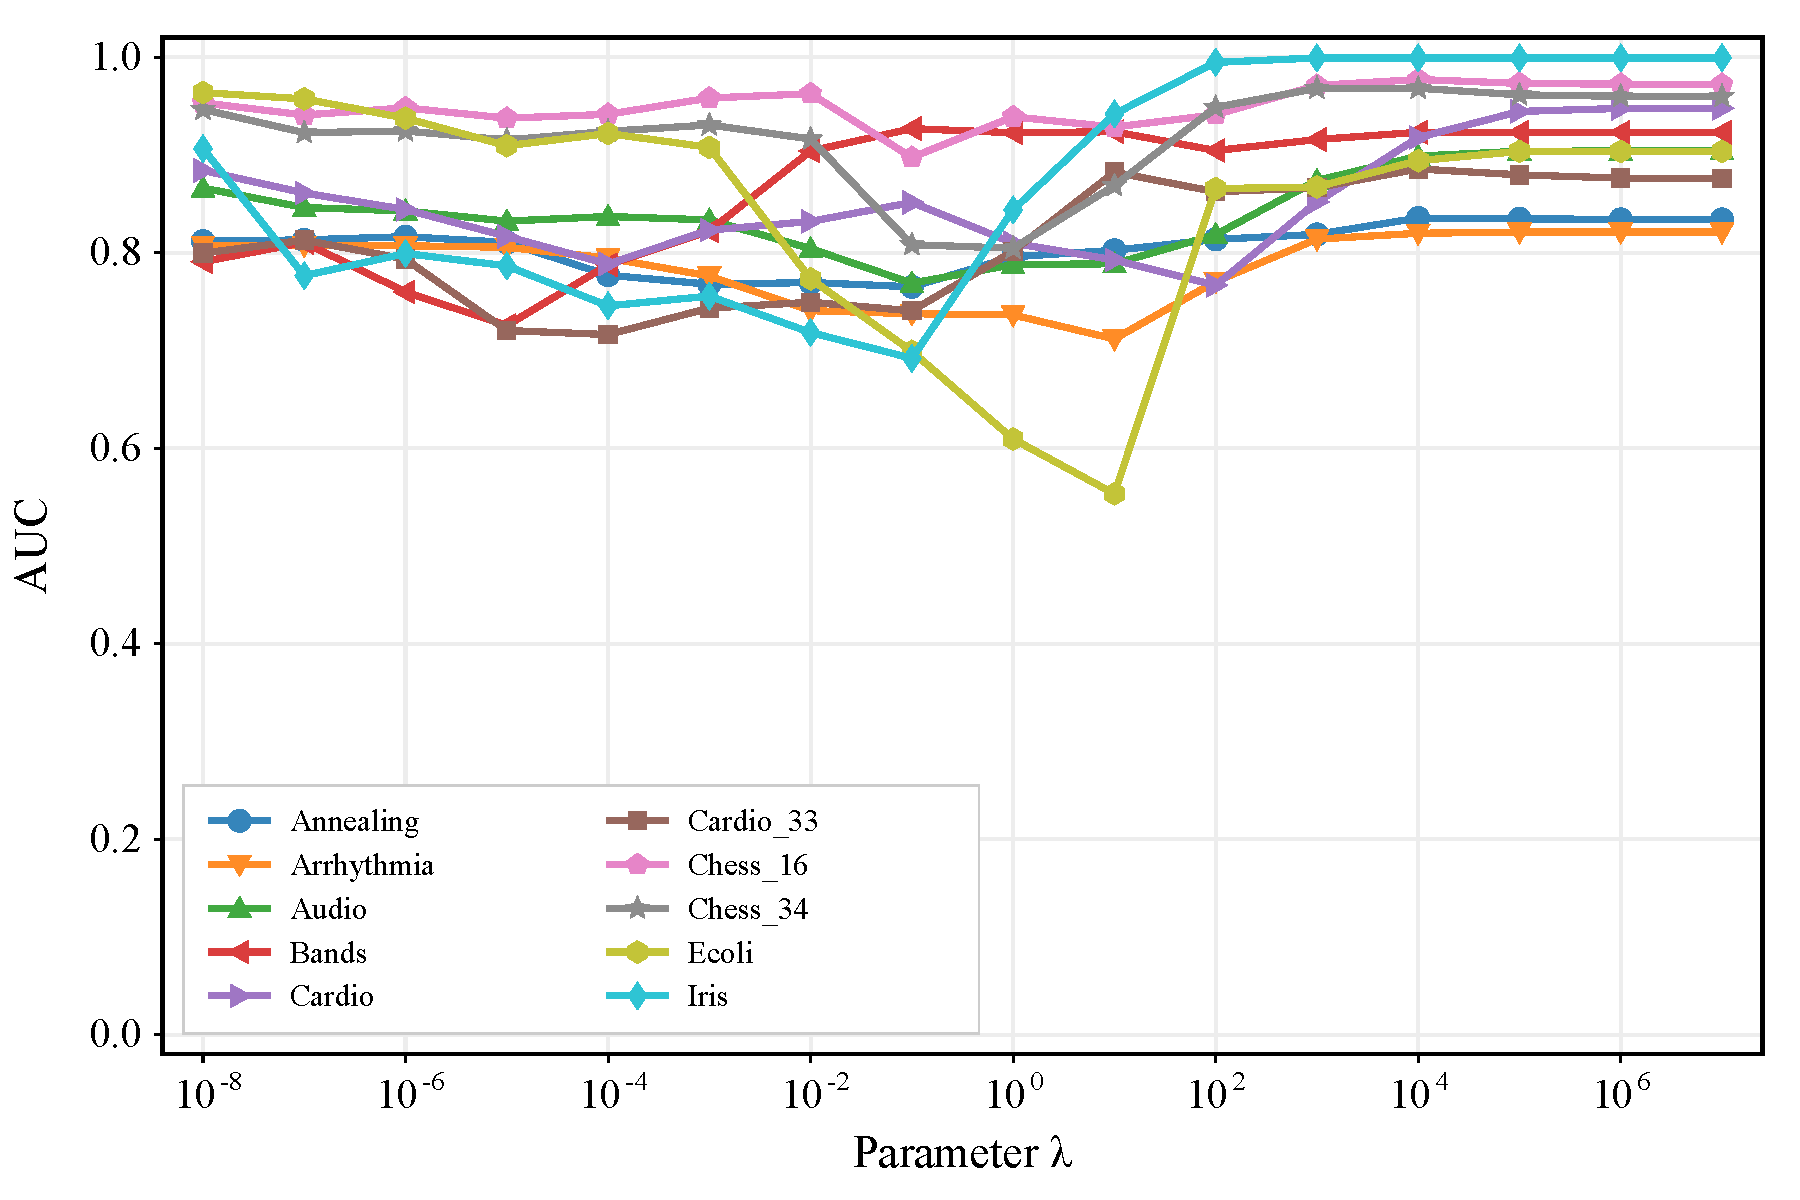
\includegraphics[width=\linewidth]{Figures/KSRA_lambda_Part1.pdf}\\
        \small (a) Datasets 1--10
        \label{fig:lambda_part1}
    \end{minipage}\hspace{8pt}%          
    \begin{minipage}[b]{0.40\textwidth}
        \centering
        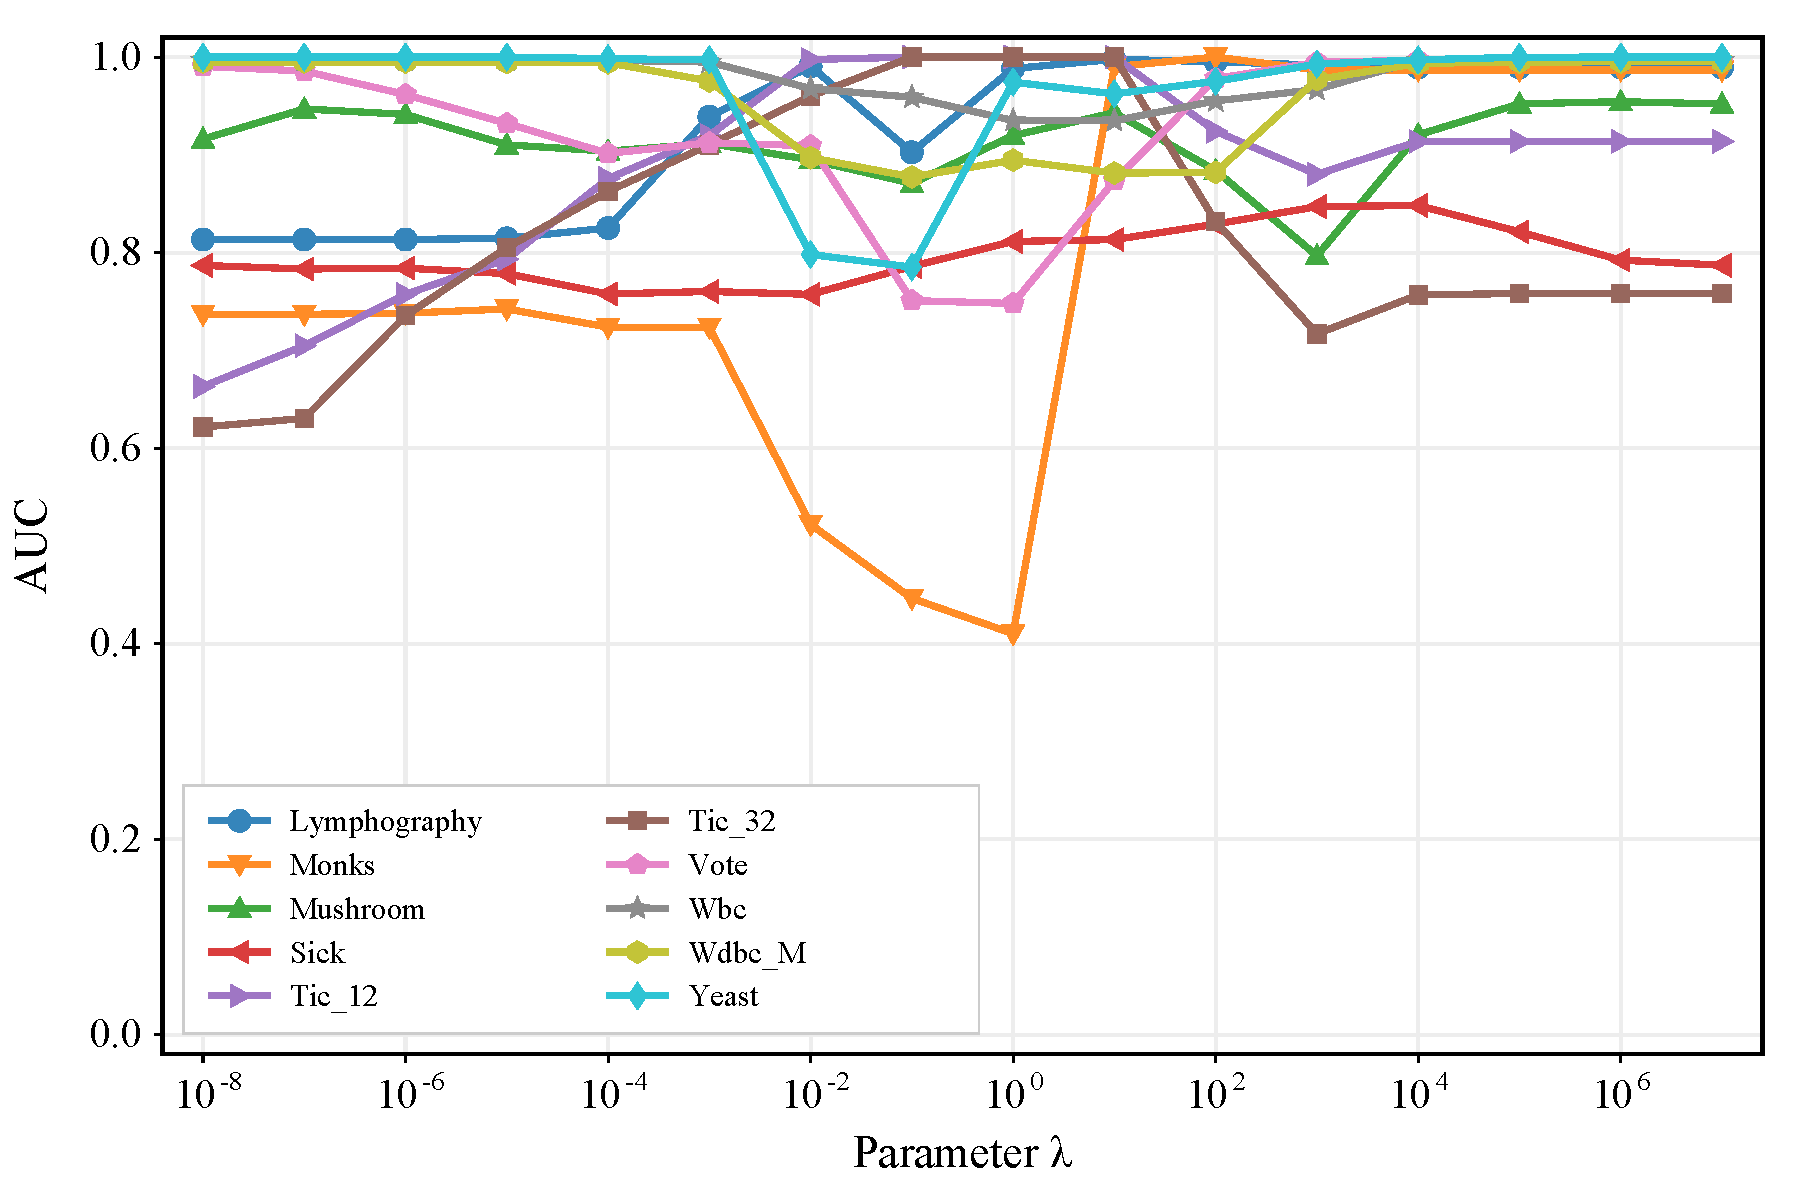
\includegraphics[width=\linewidth]{Figures/KSRA_lambda_Part2.pdf}\\
        \small (b) Datasets 11--20
        \label{fig:lambda_part2}
    \end{minipage}

    \vspace{10pt}

    % ===== 第二行 =====
    \begin{minipage}[b]{0.40\textwidth}
        \centering
        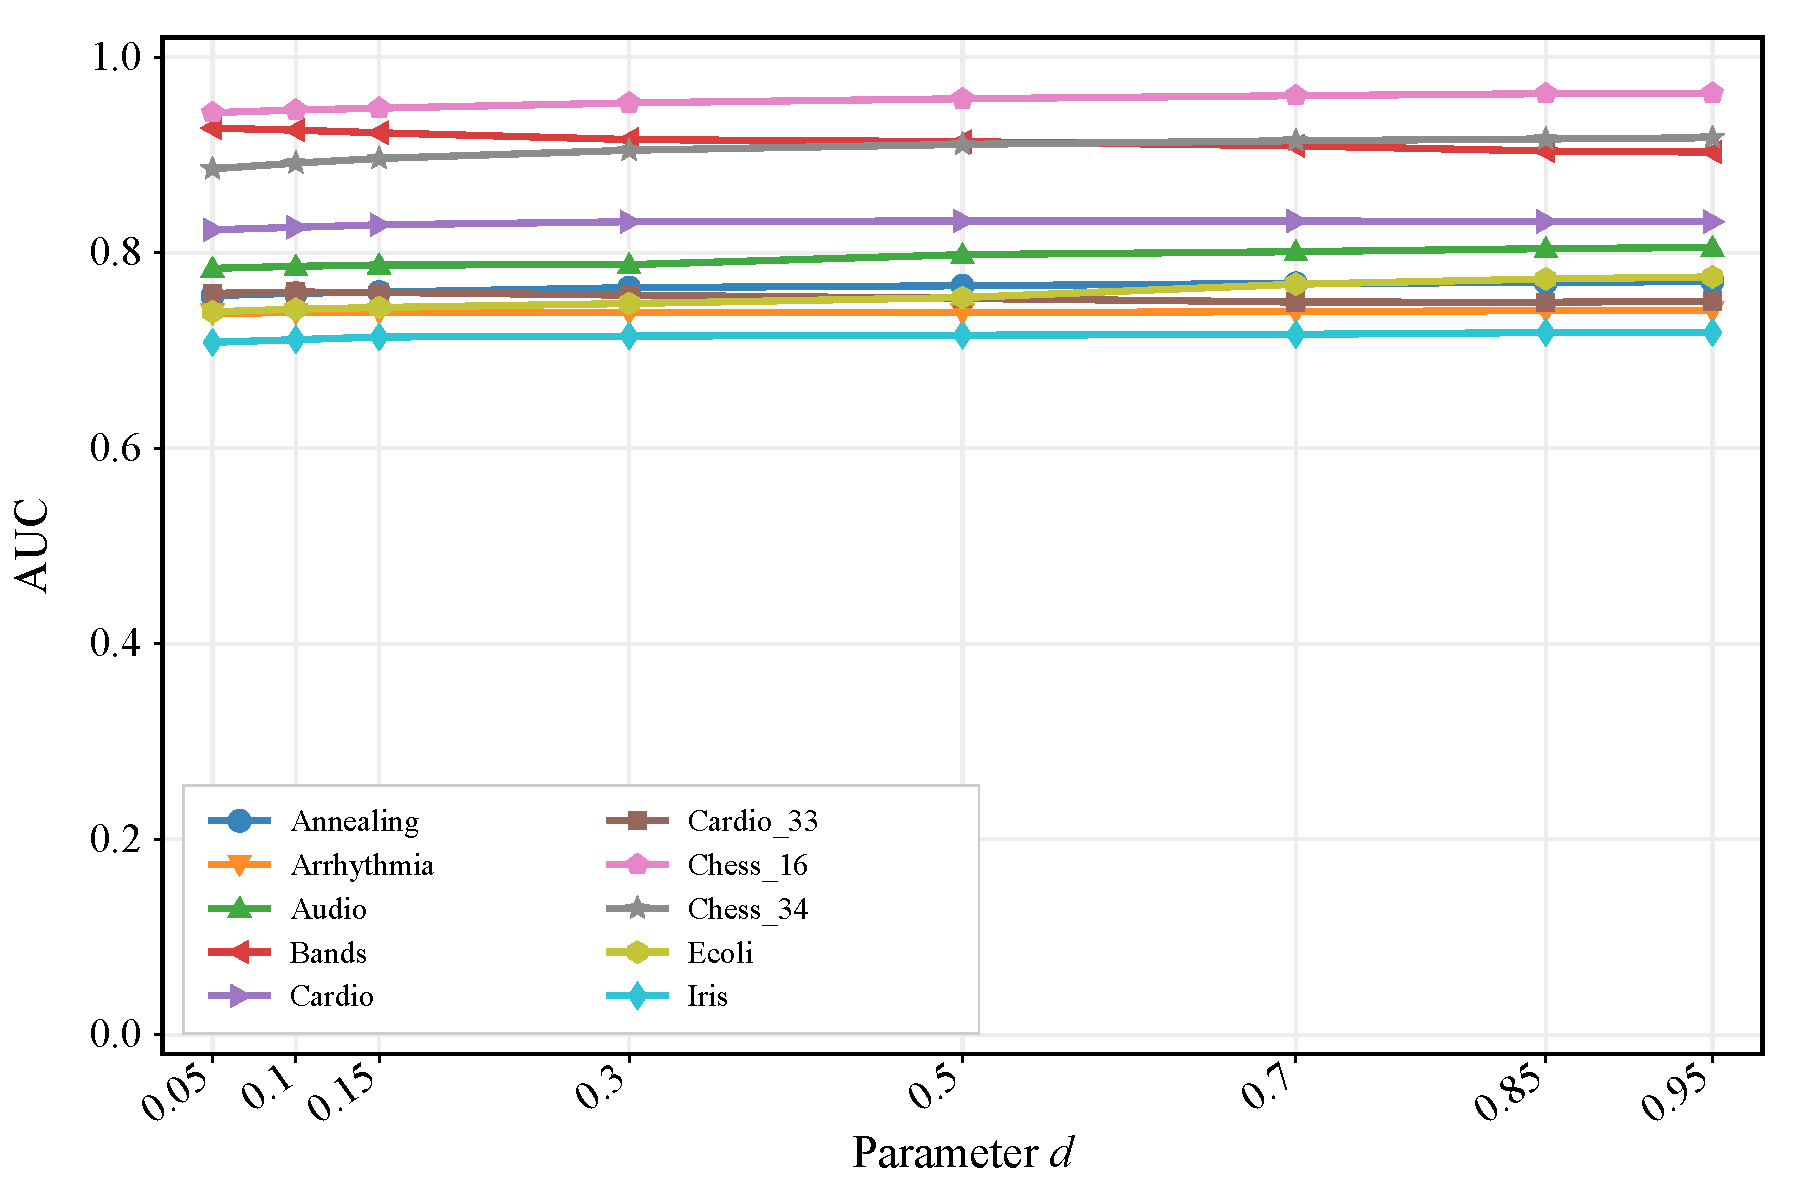
\includegraphics[width=\linewidth]{Figures/KSRA_d_Part1.pdf}\\
        \small (c) Datasets 1--10
        \label{fig:d_part1}
    \end{minipage}\hspace{8pt}%
    \begin{minipage}[b]{0.40\textwidth}
        \centering
        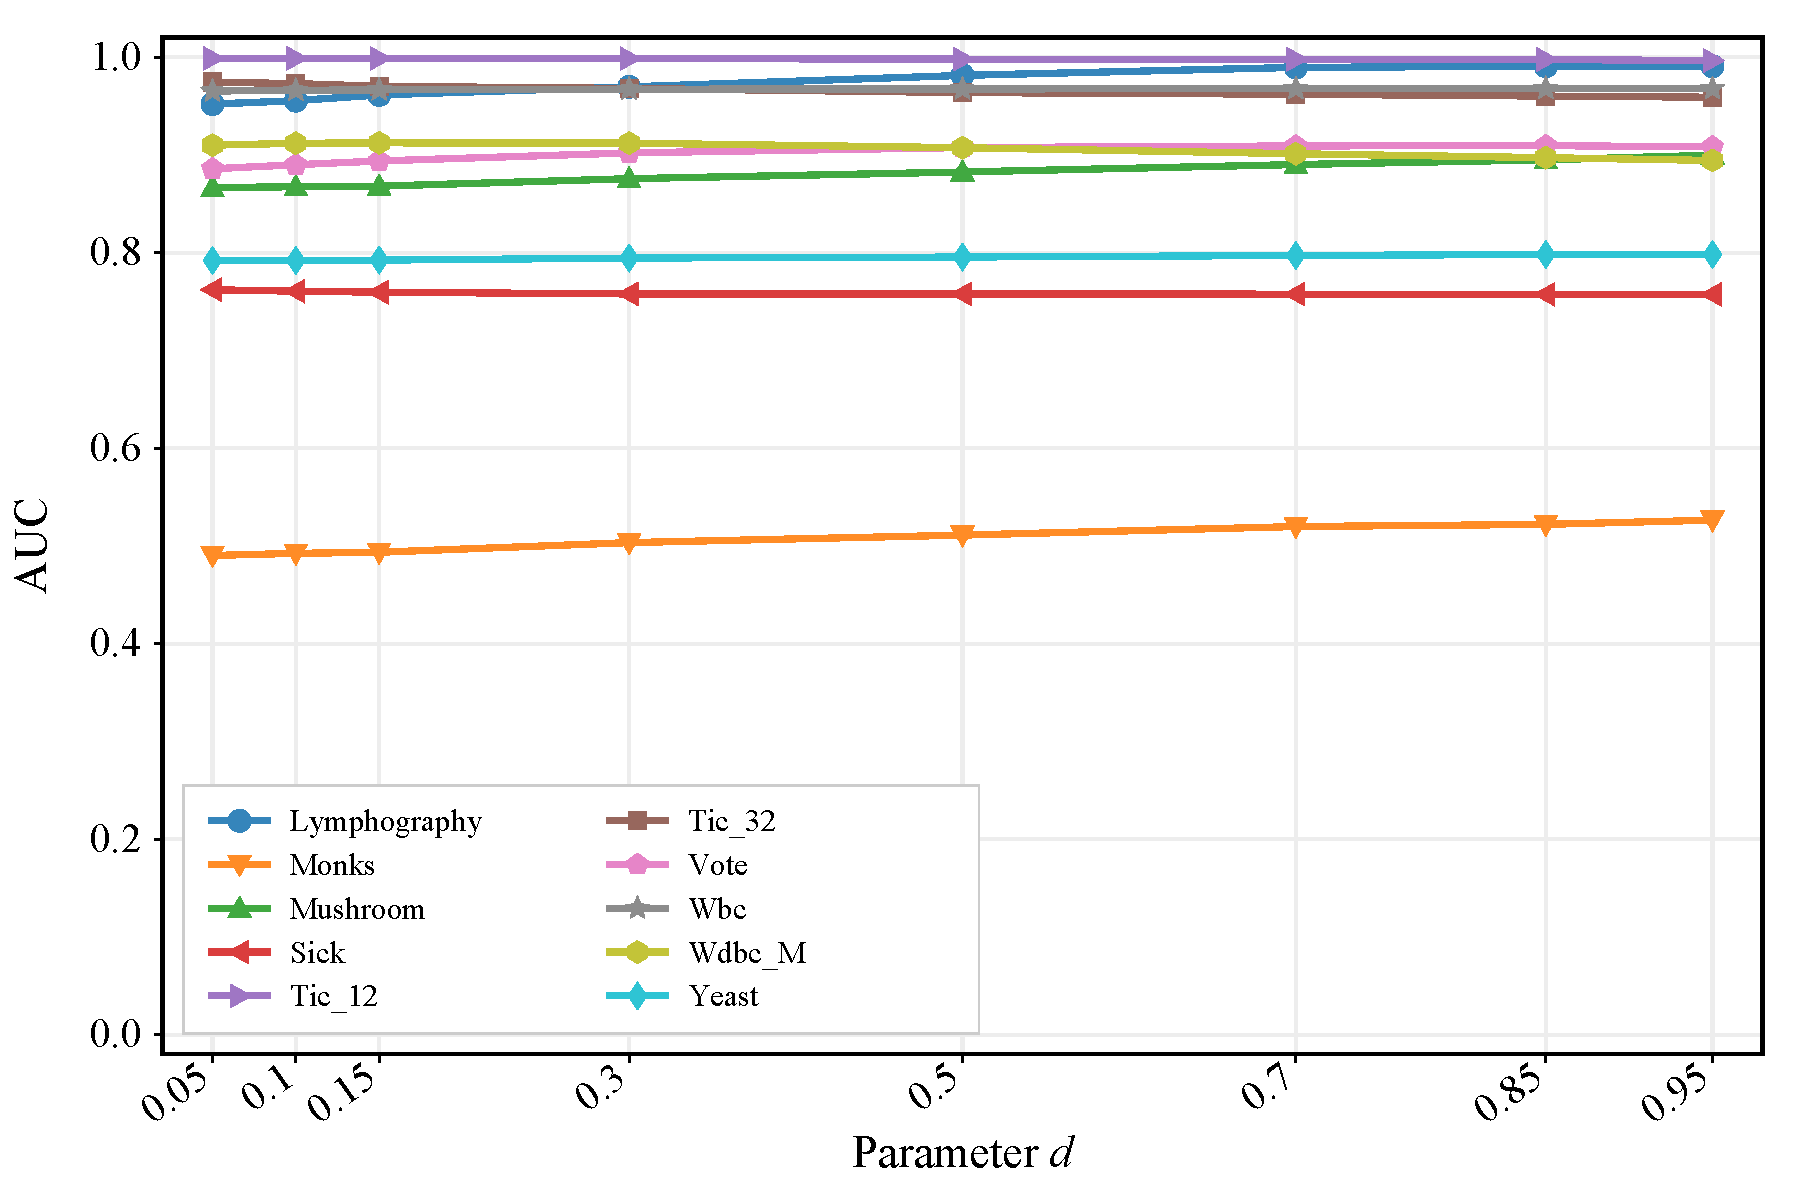
\includegraphics[width=\linewidth]{Figures/KSRA_d_Part2.pdf}\\
        \small (d) Datasets 11--20
        \label{fig:d_part2}
    \end{minipage}

    \vspace{10pt}

    % ===== 第三行 =====
    \begin{minipage}[b]{0.40\textwidth}
        \centering
        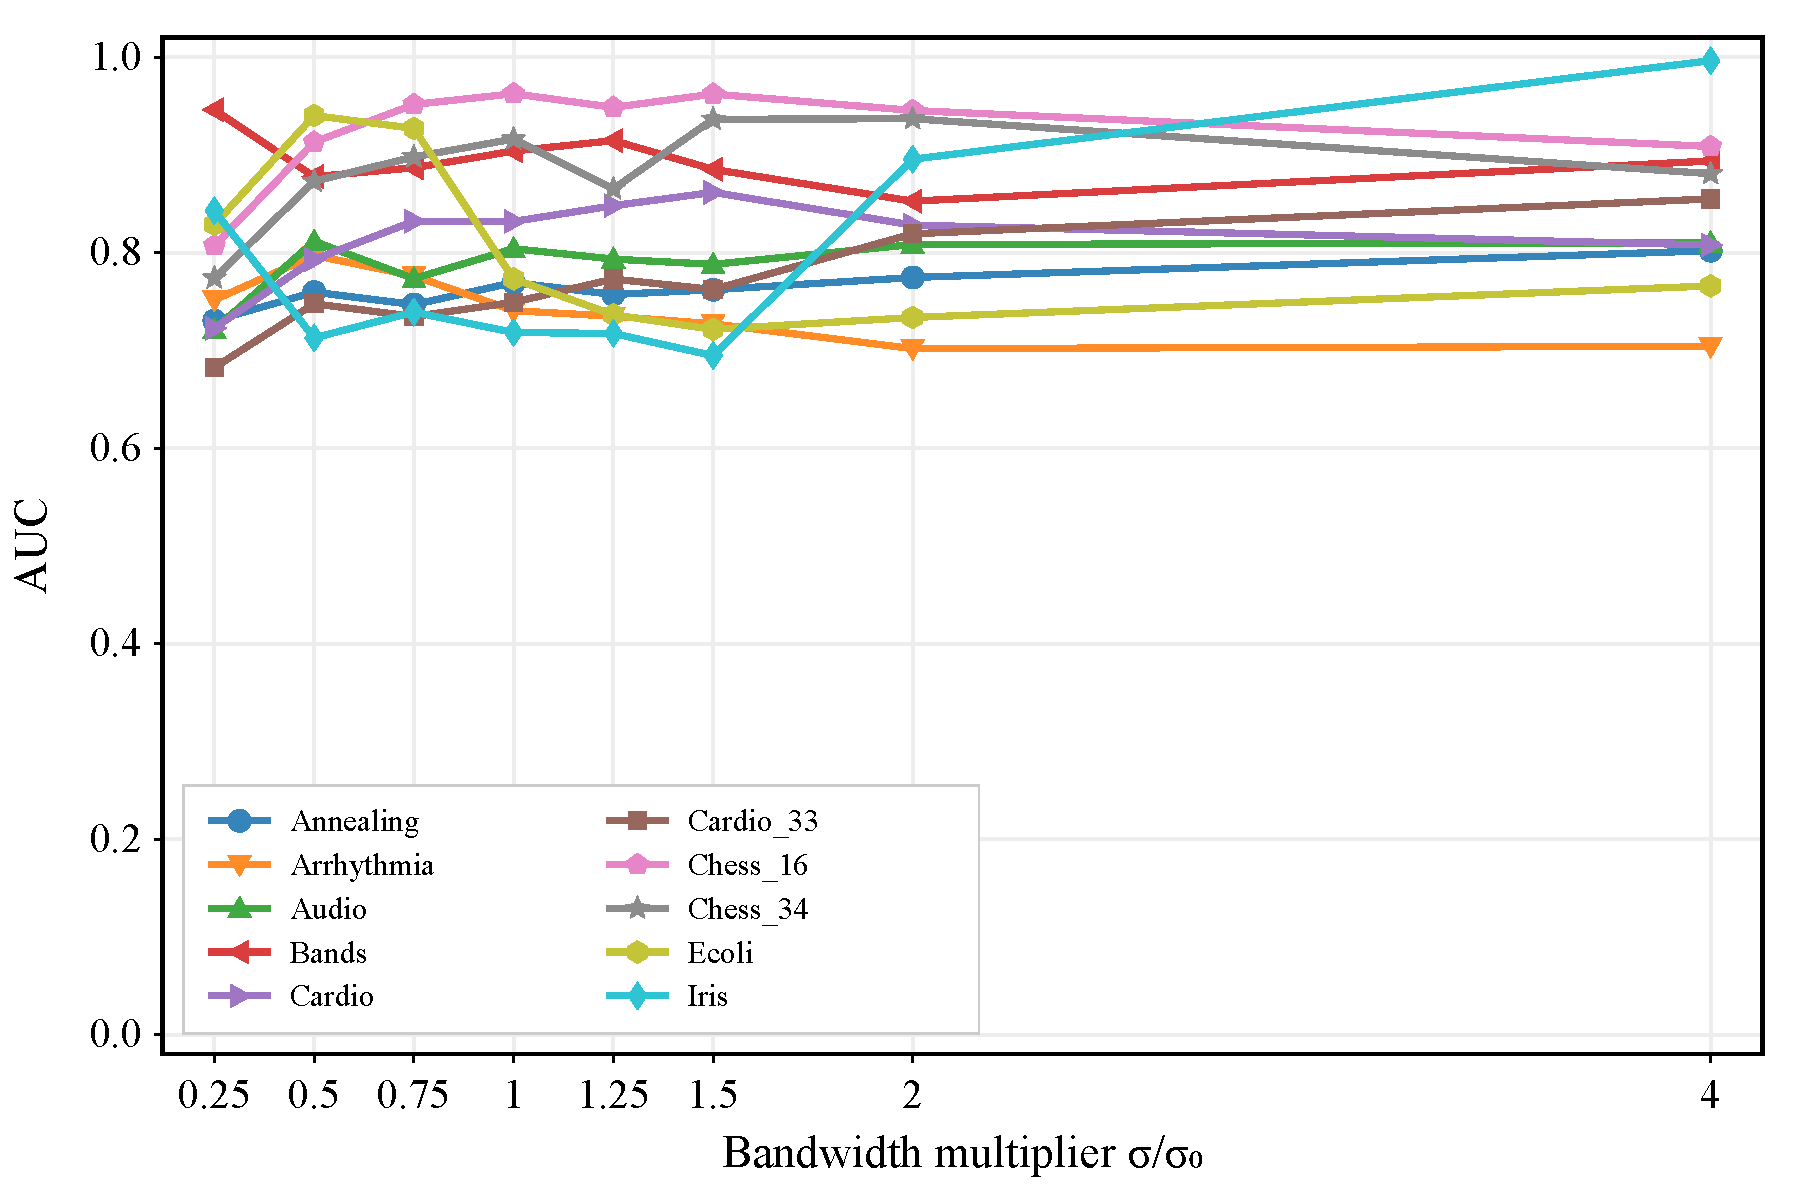
\includegraphics[width=\linewidth]{Figures/KSRA_sigma_Part1.pdf}\\
        \small (e) Datasets 1--10
        \label{fig:sigma_part1}
    \end{minipage}\hspace{8pt}%
    \begin{minipage}[b]{0.40\textwidth}
        \centering
        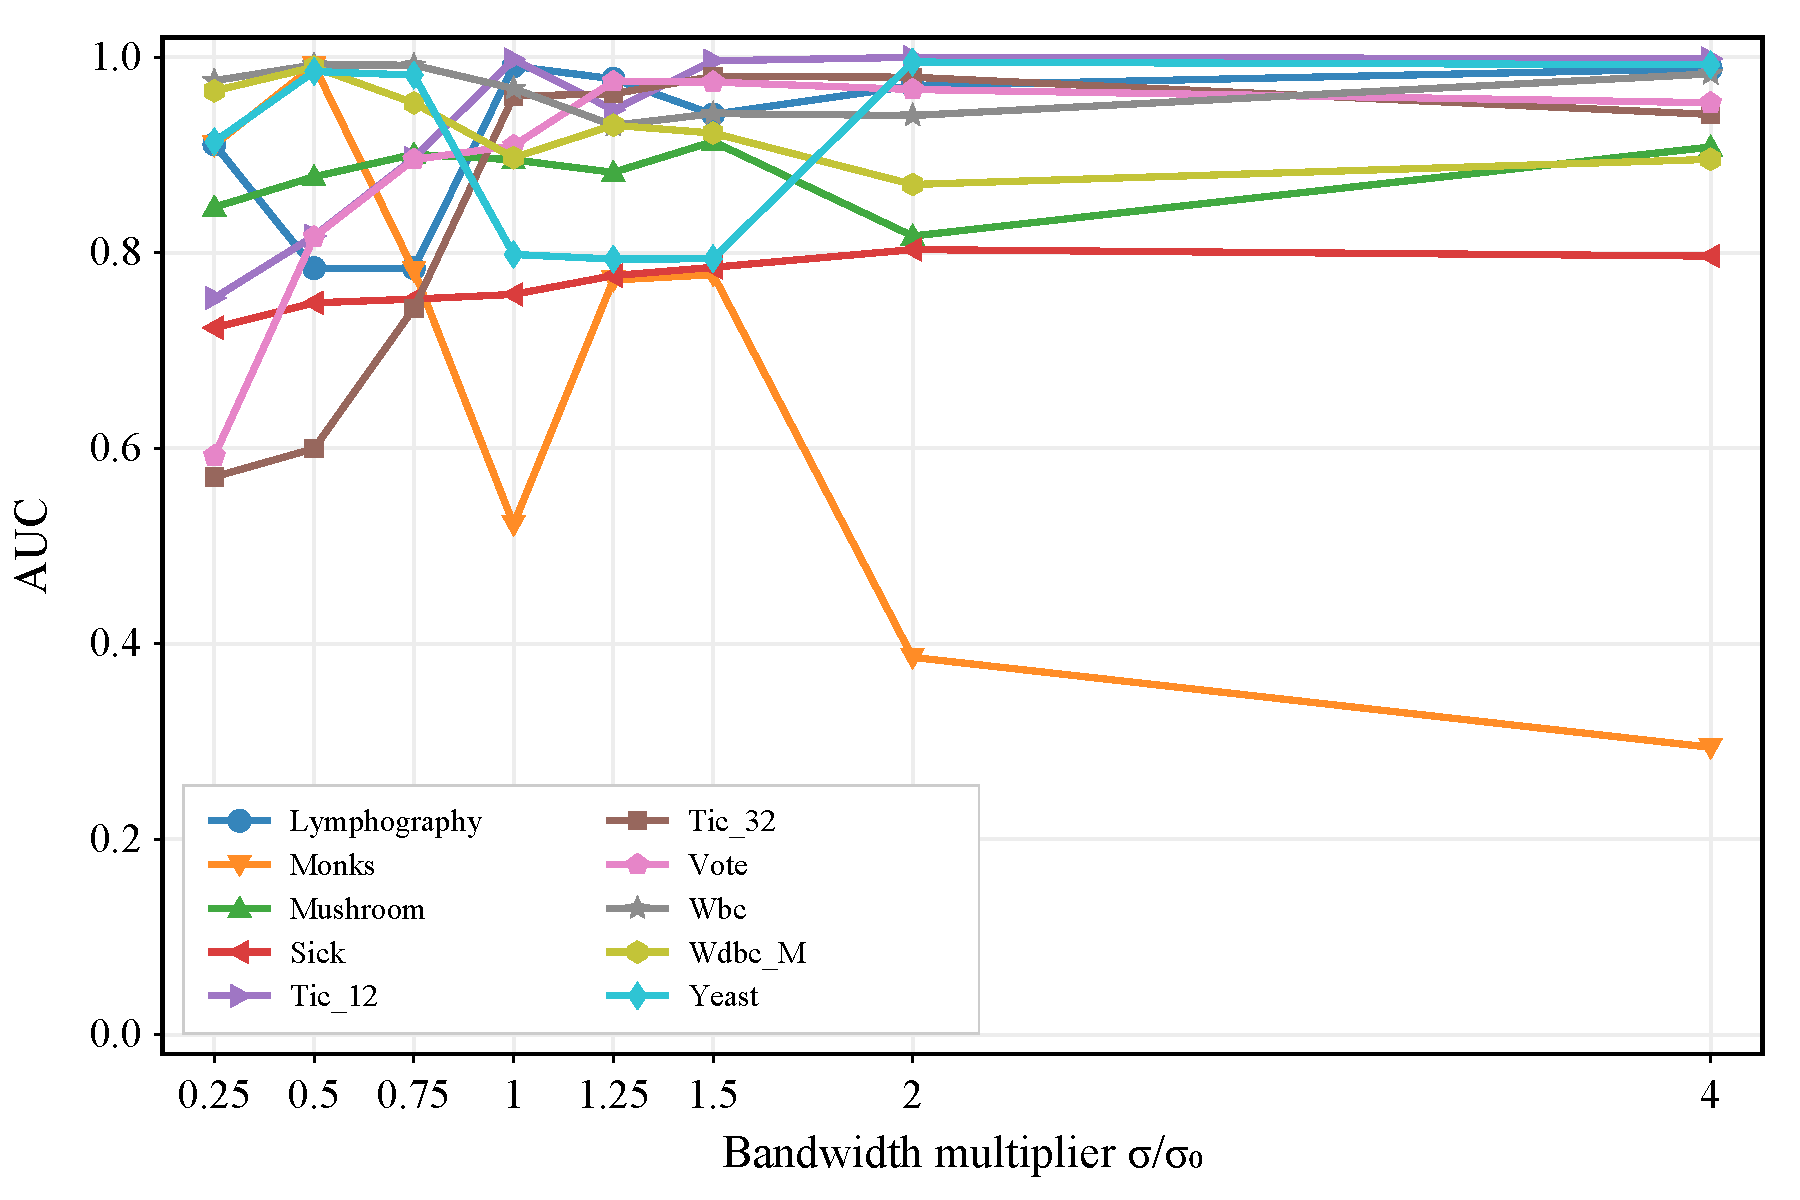
\includegraphics[width=\linewidth]{Figures/KSRA_sigma_Part2.pdf}\\
        \small (f) Datasets 11--20
        \label{fig:sigma_part2}
    \end{minipage}

    \caption{Sensitivity of KSRA to the regularization parameter $\lambda$, restart weight $d$, and kernel bandwidth multiplier $\sigma/\sigma_0$ across 20 benchmark datasets.}
    \label{fig:parameters_sensitivity}
\end{figure*}


\subsection{Ablation Experiments}

To examine the contributions of individual components, we construct three ablation variants based on the fixed KSRA$_2$ formulation, replacing one component at a time while retaining the remaining computational steps. In w/o Hybrid Kernel, the mixed-type hybrid kernel is replaced by a standard RBF kernel based on Euclidean distances. In w/o Self-Representation, the self-representation matrix is not learned; instead, the hybrid kernel matrix is directly used as the graph affinity matrix. In w/o Random Walk, PageRank-based propagation is replaced by direct degree-based graph centrality scores. Whenever self-representation is retained, both the reconstruction loss and regularization term use squared Frobenius norms, consistent with the full KSRA formulation.

All variants are evaluated on the same 10 of 20 benchmark datasets. The kernel bandwidth is set to the mean off-diagonal distance for the corresponding kernel, and the restart weight is fixed at 0.85 whenever random-walk propagation is retained. For variants retaining self-representation, $\lambda$ is independently searched over $\{10^{-8},10^{-7},\ldots,10^{7}\}$, and the best evaluation AUC is reported for each dataset. The parameter $\lambda$ is inapplicable when self-representation is removed. Thus, this study compares the best observed performance within the examined
parameter range, rather than component removal under identical parameter values.

Table~\ref{tab:ablation_illustrative_subset} summarizes the ablation results. The Difference column reports the change in mean AUC, expressed in percentage points, relative to the full KSRA model.

\begin{enumerate}[\indent (1)]
    \item Replacing the hybrid kernel reduces the mean AUC from 0.9525 to 0.9293, a decrease of 2.32 percentage points. The largest reductions occur on Sick and Tic\_32, supporting the contribution of the mixed-type kernel to the observed overall performance.

    \item Removing self-representation reduces the mean AUC to 0.9111, a decrease of 4.14 percentage points.
    The full model achieves higher AUC on 9 datasets,
    ties on 1, and lower AUC on none, supporting the
    usefulness of learning sample relationships beyond
    directly using kernel affinities.

    \item Replacing random-walk propagation with degree-based
    scoring slightly reduces the mean AUC to 0.9517,
    a decrease of 0.08 percentage points. The small observed
    difference indicates that both scoring mechanisms retain
    similar average detection performance on this subset.
\end{enumerate}

Additionally, to examine the value of jointly using density and structural information, we conducted a fusion analysis on the same ten datasets while retaining identical score components and parameter settings. The original multiplicative fusion achieves a mean AUC of 0.9525, exceeding the structural score alone (0.9059) and the density weight alone (0.9111), supporting their complementary value on the datasets. Uniform restart assigns equal restart input to all nodes, whereas $\boldsymbol w$ introduces isolation information at the final scoring stage. Using normalized $\boldsymbol w$ as the restart distribution would instead favor restarting at potentially isolated nodes and constitutes a different design.

\begin{table*}[!ht]
	\centering
	\caption{Ablation study results of KSRA in terms of average AUC across the 10 benchmark datasets.}\label{tab:ablation_illustrative_subset}
	\resizebox{1\textwidth}{!}{
		\begin{tabular}{lcccccccccccc}
			\toprule
			Method & Arrhythmia & Cardio\_33 & Chess\_16 & Monks & Sick & Tic\_12 & Tic\_32 & Vote & Wbc & Yeast & Average & Difference \\
			\midrule
			KSRA & \textbf{0.821} & \textbf{0.886} & \textbf{0.977} & \textbf{1.000} & \textbf{0.848} & \textbf{1.000} & \textbf{1.000} & \textbf{0.997} & \textbf{0.997} & \textbf{1.000} & \textbf{0.953} & 0.00\% \\
			w/o Hybrid Kernel & 0.805 & \textbf{0.886} & 0.964 & \textbf{1.000} & 0.798 & 0.962 & 0.888 & 0.995 & \textbf{0.997} & \textbf{1.000} & 0.929 & -2.32\% \\
			w/o Self-Representation & 0.819 & 0.878 & 0.973 & 0.987 & 0.797 & 0.914 & 0.758 & \textbf{0.997} & 0.995 & 0.995 & 0.911 & -4.14\% \\
			w/o Random Walk & \textbf{0.821} & 0.883 & 0.975 & \textbf{1.000} & 0.845 & \textbf{1.000} & \textbf{1.000} & 0.997 & 0.997 & \textbf{1.000} & 0.952 & -0.08\% \\
			\bottomrule
		\end{tabular}
	}
\end{table*}

\subsection{Distance Concentration and Kernel-Profile Representation}

To examine changes in distances and kernel representations with increasing irrelevant dimensionality, we fixed the sample size at 500, with 20 numerical and 10 categorical base features. We appended 0, 20, 50, 100, 200, and 500 independent irrelevant numerical features. Both structureless data and structured data containing 5\% anomalies were considered, using five data-generation seeds per setting. Kernel bandwidths were determined by the mean off-diagonal distance.

Fig.\ref{fig:distance_concentration_geometry}(a) and (b) show the distance coefficient of variation (CV) for the two scenarios. Here, kernel-profile distance denotes the Euclidean distance between kernel-matrix rows, characterizing the representations supplied to self-representation learning. Higher CV indicates greater relative distance dispersion. Fig.\ref{fig:distance_concentration_geometry}(c) additionally reports the standardized class-separation measure:
\begin{equation*}
    G=
\frac{\mu_{\mathrm{NA}}-\mu_{\mathrm{NN}}}
{\sqrt{(s_{\mathrm{NA}}^2+s_{\mathrm{NN}}^2)/2}},
\end{equation*}
where NA and NN denote normal–anomaly and normal–normal sample pairs, respectively, and $\mu$ and $s$ are the corresponding distance means and standard deviations. Larger positive values indicate clearer distance separation between the two pair types. Curves report means and standard deviations across five repetitions. The measure $G$ is descriptive; overlapping sample pairs are not treated as independent statistical observations.

\begin{enumerate}
    \item Original distances exhibit increasing concentration as irrelevant dimensions are added. Distance CV decreases in both scenarios. For structured data, increasing the total dimensionality from 30 to 530 reduces the mixed-distance CV from 0.3181 to 0.0350, indicating diminished relative distance differences.

    \item Kernel profiles retain greater relative distance variation. At 530 dimensions, hybrid-kernel profiles achieve distance CV values of 0.0514 and 0.1842 on structureless and structured data, respectively, compared with 0.0276 and 0.0350 for the corresponding original mixed distances. Thus, kernel profiles retain greater relative geometric dispersion even when the original distances become concentrated.

    \item The greater relative dispersion is accompanied by observable class-separation information. On structured data at 530 dimensions, the hybrid-kernel profiles achieve a standardized separation of 3.5860, exceeding the original mixed-distance value of 2.3121. Nevertheless, this separation decreases with increasing irrelevant dimensionality, and Euclidean-kernel profiles also exhibit corresponding benefits. 
\end{enumerate}

These observations concern representation geometry under the tested conditions; greater distance dispersion does not by itself guarantee improved anomaly detection.


\begin{figure*}[t]
    \centering
    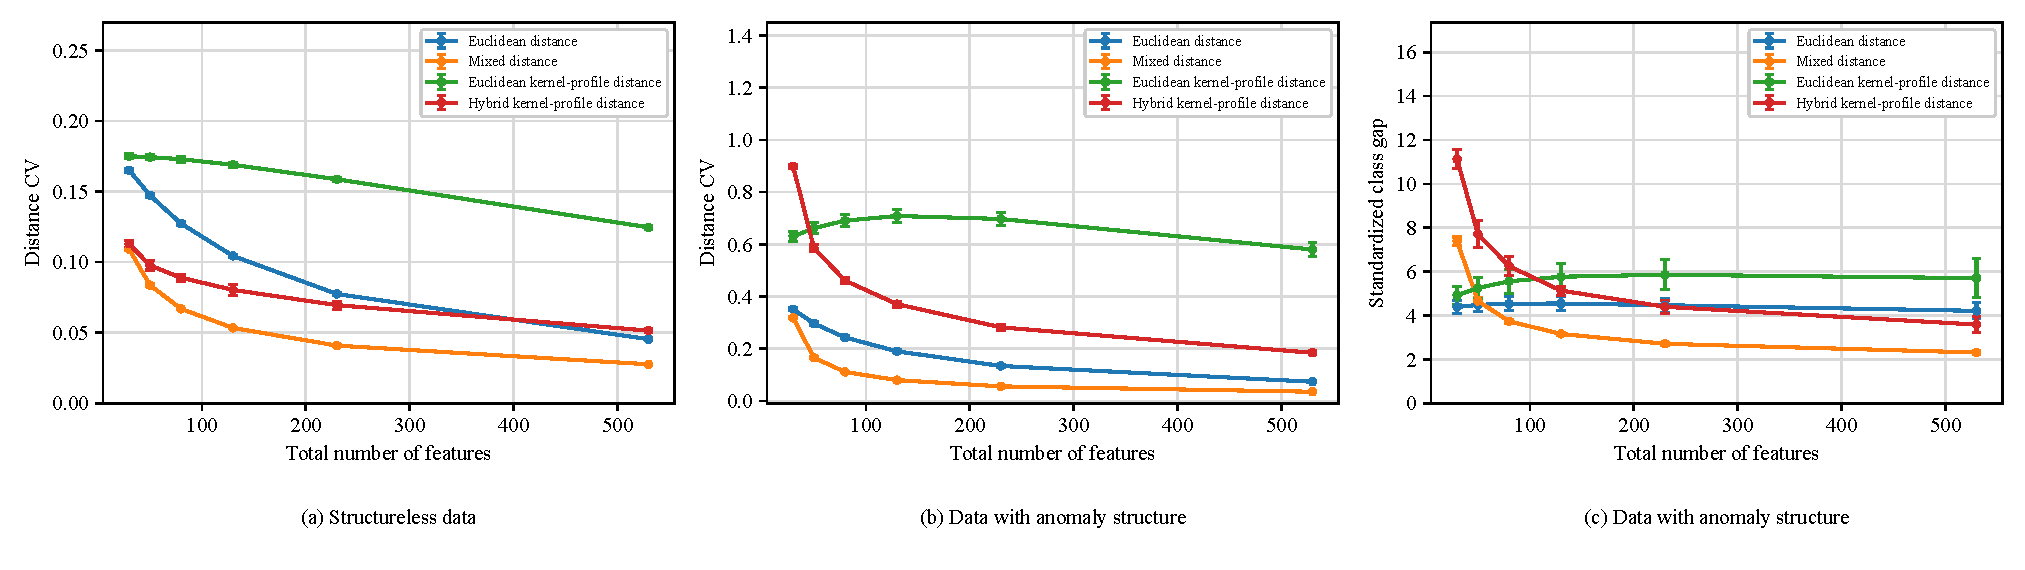
\includegraphics[width=\textwidth]
    {Figures/concentration_geometry_panel_updated.pdf}
    \caption{
        Distance dispersion and class separation with increasing
        irrelevant dimensionality:
        (a) distance CV on structureless data;
        (b) distance CV on structured data; and
        (c) standardized class separation on structured data.
        Kernel-profile distances are Euclidean distances between
        kernel-matrix rows.
        Error bars indicate standard deviations across five
        data-generation seeds.
    }
    \label{fig:distance_concentration_geometry}
\end{figure*}


\subsection{Computational Complexity and Scalability Analysis}

Let $n$ denote the number of samples, $m$ the number of features, $q$ the number of categorical features, and $T$ the number of random-walk iterations. The shared distance and kernel construction and random-walk propagation require $O(n^2m+Tn^2)$ time. For self-representation, KSRA$_2$ requires one dense linear-system solve with an $O(n^3)$ cost. KSRA$_1$ and KSRA$_3$ use IRLS, requiring $O(L_1n^3)$ and $O(L_3n^3)$, respectively. KSRA$_4$ uses ADMM with an $O((L_4+1)n^3)$ cost, where $L_i$ denotes the actual optimization iteration count.

All four variants store dense matrices, while the current broadcasting implementation of categorical distances additionally creates $n\times n\times q$ temporary arrays. The overall space complexity is therefore $O(nm+n^2+n^2q)$, corresponding to quadratic memory growth in $n$ for fixed feature dimensions. The following experiment evaluates the practical computational cost of the fixed KSRA$_2$ used in the main comparison.

To evaluate the computational cost of KSRA with increasing sample size, we generated synthetic mixed data containing 20 numerical features and 10 categorical features with four levels each. Sample sizes were set to 250, 500, 1000, 2000, 3000, and 4000. The variant KSRA$_2$ was used throughout, with $\lambda=0.01$, random-walk restart weight $d=0.85$, and kernel bandwidth determined by the mean off-diagonal mixed distance. Five random seeds were planned for each sample size. Each run used a fresh subprocess with numerical-library threads limited to one. Experiments were conducted on an Intel Core i5-1035G1 CPU with approximately 16 GiB RAM and Python 3.8.20. We recorded algorithm execution time and process peak memory. Algorithm timing excluded imports, data generation, warm-up, and file I/O, whereas process peak memory included runtime overhead. A process-memory safeguard of 2335 MiB was applied.

The results show stable execution times across repeated runs at the completed sample sizes, while the time and memory costs of the current dense implementation increase substantially with sample size.

\begin{enumerate}[\indent (1)]
    \item All 25 runs from $n=250$ to $n=3000$ completed successfully. Mean execution time increased from 0.013 s to 5.009 s, with limited variation across repeated runs at each size.

    \item Self-representation became the dominant computational cost, accounting for approximately 77.0\% of total execution time at $n=3000$, whereas random-walk propagation accounted for approximately 0.16\%. This observation is consistent with the higher theoretical cost of dense self-representation.

    \item Mean peak working-set memory increased from 71.4 MiB to 1504.1 MiB. At $n=4000$, the first run was terminated because peak commit exceeded the predefined budget, and the remaining repetitions were skipped, revealing a memory constraint on the scalability of the current implementation.
\end{enumerate}

These trends arise from the dense distance, kernel, and self-representation matrices, together with broadcasting temporaries used for categorical distances. The experiment therefore supports computational feasibility at the tested smaller sample sizes while identifying limitations for larger datasets. Blockwise distance computation, kernel approximation, and scalable self-representation solvers warrant further investigation.





\section{Conclusions}\label{Conclusions}

To address the drawbacks of existing anomaly detection methods, including the curse of dimensionality and limited capacity for heterogeneous data processing, this paper proposes a novel KSRA detection model. We systematically explore multiple combinations of objective function paradigms and integrate the random walk mechanism to derive a globally discriminative anomaly representation. Extensive experiments demonstrate that KSRA achieves state-of-the-art performance on 14 out of 20 benchmark datasets. Compared with most contemporary baseline methods, its performance gains are statistically significant. Nevertheless, experimental results reveal two main limitations of the proposed model. First, its detection performance is largely dependent on the selection of hyperparameters. Second, the model incurs heavy computational and storage overhead when handling ultra-large-scale datasets. In future research, we will explore adaptive parameter optimization mechanisms, such as the automatic selection of parameter $\sigma$. Additionally, anchor learning and kernel approximation techniques will be introduced to reduce the computational complexity of the algorithm and improve its applicability to large-scale streaming data scenarios.


%\backmatter

\bmsubsection*{Acknowledgments}
This work was supported by the National Natural Science Foundation of China (62306196 and 12501439) and Sichuan Science and Technology Program (2026NSFSC0783).

\bmsubsection*{Financial Disclosure}

None reported.

\bmsubsection*{Conflicts of Interest}

The authors declare no conflicts of interest.

\bibliography{wileyNJD-Chicago}


\end{document}
